% Options for packages loaded elsewhere
\PassOptionsToPackage{unicode}{hyperref}
\PassOptionsToPackage{hyphens}{url}
%
\documentclass[
]{latex/krantz}
\usepackage{amsmath,amssymb}
\usepackage{iftex}
\ifPDFTeX
  \usepackage[T1]{fontenc}
  \usepackage[utf8]{inputenc}
  \usepackage{textcomp} % provide euro and other symbols
\else % if luatex or xetex
  \usepackage{unicode-math} % this also loads fontspec
  \defaultfontfeatures{Scale=MatchLowercase}
  \defaultfontfeatures[\rmfamily]{Ligatures=TeX,Scale=1}
\fi
\usepackage{lmodern}
\ifPDFTeX\else
  % xetex/luatex font selection
\fi
% Use upquote if available, for straight quotes in verbatim environments
\IfFileExists{upquote.sty}{\usepackage{upquote}}{}
\IfFileExists{microtype.sty}{% use microtype if available
  \usepackage[]{microtype}
  \UseMicrotypeSet[protrusion]{basicmath} % disable protrusion for tt fonts
}{}
\makeatletter
\@ifundefined{KOMAClassName}{% if non-KOMA class
  \IfFileExists{parskip.sty}{%
    \usepackage{parskip}
  }{% else
    \setlength{\parindent}{0pt}
    \setlength{\parskip}{6pt plus 2pt minus 1pt}}
}{% if KOMA class
  \KOMAoptions{parskip=half}}
\makeatother
\usepackage{xcolor}
\usepackage{color}
\usepackage{fancyvrb}
\newcommand{\VerbBar}{|}
\newcommand{\VERB}{\Verb[commandchars=\\\{\}]}
\DefineVerbatimEnvironment{Highlighting}{Verbatim}{commandchars=\\\{\}}
% Add ',fontsize=\small' for more characters per line
\usepackage{framed}
\definecolor{shadecolor}{RGB}{248,248,248}
\newenvironment{Shaded}{\begin{snugshade}}{\end{snugshade}}
\newcommand{\AlertTok}[1]{\textcolor[rgb]{0.94,0.16,0.16}{#1}}
\newcommand{\AnnotationTok}[1]{\textcolor[rgb]{0.56,0.35,0.01}{\textbf{\textit{#1}}}}
\newcommand{\AttributeTok}[1]{\textcolor[rgb]{0.13,0.29,0.53}{#1}}
\newcommand{\BaseNTok}[1]{\textcolor[rgb]{0.00,0.00,0.81}{#1}}
\newcommand{\BuiltInTok}[1]{#1}
\newcommand{\CharTok}[1]{\textcolor[rgb]{0.31,0.60,0.02}{#1}}
\newcommand{\CommentTok}[1]{\textcolor[rgb]{0.56,0.35,0.01}{\textit{#1}}}
\newcommand{\CommentVarTok}[1]{\textcolor[rgb]{0.56,0.35,0.01}{\textbf{\textit{#1}}}}
\newcommand{\ConstantTok}[1]{\textcolor[rgb]{0.56,0.35,0.01}{#1}}
\newcommand{\ControlFlowTok}[1]{\textcolor[rgb]{0.13,0.29,0.53}{\textbf{#1}}}
\newcommand{\DataTypeTok}[1]{\textcolor[rgb]{0.13,0.29,0.53}{#1}}
\newcommand{\DecValTok}[1]{\textcolor[rgb]{0.00,0.00,0.81}{#1}}
\newcommand{\DocumentationTok}[1]{\textcolor[rgb]{0.56,0.35,0.01}{\textbf{\textit{#1}}}}
\newcommand{\ErrorTok}[1]{\textcolor[rgb]{0.64,0.00,0.00}{\textbf{#1}}}
\newcommand{\ExtensionTok}[1]{#1}
\newcommand{\FloatTok}[1]{\textcolor[rgb]{0.00,0.00,0.81}{#1}}
\newcommand{\FunctionTok}[1]{\textcolor[rgb]{0.13,0.29,0.53}{\textbf{#1}}}
\newcommand{\ImportTok}[1]{#1}
\newcommand{\InformationTok}[1]{\textcolor[rgb]{0.56,0.35,0.01}{\textbf{\textit{#1}}}}
\newcommand{\KeywordTok}[1]{\textcolor[rgb]{0.13,0.29,0.53}{\textbf{#1}}}
\newcommand{\NormalTok}[1]{#1}
\newcommand{\OperatorTok}[1]{\textcolor[rgb]{0.81,0.36,0.00}{\textbf{#1}}}
\newcommand{\OtherTok}[1]{\textcolor[rgb]{0.56,0.35,0.01}{#1}}
\newcommand{\PreprocessorTok}[1]{\textcolor[rgb]{0.56,0.35,0.01}{\textit{#1}}}
\newcommand{\RegionMarkerTok}[1]{#1}
\newcommand{\SpecialCharTok}[1]{\textcolor[rgb]{0.81,0.36,0.00}{\textbf{#1}}}
\newcommand{\SpecialStringTok}[1]{\textcolor[rgb]{0.31,0.60,0.02}{#1}}
\newcommand{\StringTok}[1]{\textcolor[rgb]{0.31,0.60,0.02}{#1}}
\newcommand{\VariableTok}[1]{\textcolor[rgb]{0.00,0.00,0.00}{#1}}
\newcommand{\VerbatimStringTok}[1]{\textcolor[rgb]{0.31,0.60,0.02}{#1}}
\newcommand{\WarningTok}[1]{\textcolor[rgb]{0.56,0.35,0.01}{\textbf{\textit{#1}}}}
\usepackage{longtable,booktabs,array}
\usepackage{calc} % for calculating minipage widths
% Correct order of tables after \paragraph or \subparagraph
\usepackage{etoolbox}
\makeatletter
\patchcmd\longtable{\par}{\if@noskipsec\mbox{}\fi\par}{}{}
\makeatother
% Allow footnotes in longtable head/foot
\IfFileExists{footnotehyper.sty}{\usepackage{footnotehyper}}{\usepackage{footnote}}
\makesavenoteenv{longtable}
\usepackage{graphicx}
\makeatletter
\def\maxwidth{\ifdim\Gin@nat@width>\linewidth\linewidth\else\Gin@nat@width\fi}
\def\maxheight{\ifdim\Gin@nat@height>\textheight\textheight\else\Gin@nat@height\fi}
\makeatother
% Scale images if necessary, so that they will not overflow the page
% margins by default, and it is still possible to overwrite the defaults
% using explicit options in \includegraphics[width, height, ...]{}
\setkeys{Gin}{width=\maxwidth,height=\maxheight,keepaspectratio}
% Set default figure placement to htbp
\makeatletter
\def\fps@figure{htbp}
\makeatother
\setlength{\emergencystretch}{3em} % prevent overfull lines
\providecommand{\tightlist}{%
  \setlength{\itemsep}{0pt}\setlength{\parskip}{0pt}}
\setcounter{secnumdepth}{5}
\usepackage[portuguese]{babel}

\usepackage{booktabs}
\usepackage{longtable}
\usepackage[bf,singlelinecheck=off]{caption}

\usepackage{Alegreya}
\usepackage[scale=.7]{sourcecodepro}

\usepackage{framed,color}
\definecolor{shadecolor}{RGB}{248,248,248}

\renewcommand{\textfraction}{0.05}
\renewcommand{\topfraction}{0.8}
\renewcommand{\bottomfraction}{0.8}
\renewcommand{\floatpagefraction}{0.75}

\renewenvironment{quote}{\begin{VF}}{\end{VF}}
\usepackage{hyperref}
\let\oldhref\href
\renewcommand{\href}[2]{#2\footnote{\url{#1}}}

\ifxetex
  \usepackage{letltxmacro}
  \setlength{\XeTeXLinkMargin}{1pt}
  \LetLtxMacro\SavedIncludeGraphics\includegraphics
  \def\includegraphics#1#{% #1 catches optional stuff (star/opt. arg.)
    \IncludeGraphicsAux{#1}%
  }%
  \newcommand*{\IncludeGraphicsAux}[2]{%
    \XeTeXLinkBox{%
      \SavedIncludeGraphics#1{#2}%
    }%
  }%
\fi

\makeatletter
\newenvironment{kframe}{%
\medskip{}
\setlength{\fboxsep}{.8em}
 \def\at@end@of@kframe{}%
 \ifinner\ifhmode%
  \def\at@end@of@kframe{\end{minipage}}%
  \begin{minipage}{\columnwidth}%
 \fi\fi%
 \def\FrameCommand##1{\hskip\@totalleftmargin \hskip-\fboxsep
 \colorbox{shadecolor}{##1}\hskip-\fboxsep
     % There is no \\@totalrightmargin, so:
     \hskip-\linewidth \hskip-\@totalleftmargin \hskip\columnwidth}%
 \MakeFramed {\advance\hsize-\width
   \@totalleftmargin\z@ \linewidth\hsize
   \@setminipage}}%
 {\par\unskip\endMakeFramed%
 \at@end@of@kframe}
\makeatother

\makeatletter
\@ifundefined{Shaded}{
}{\renewenvironment{Shaded}{\begin{kframe}}{\end{kframe}}}
\makeatother

\newenvironment{rmdblock}[1]
  {
  \begin{itemize}
  \renewcommand{\labelitemi}{
    \raisebox{-.7\height}[0pt][0pt]{
      {\setkeys{Gin}{width=3em,keepaspectratio}\includegraphics{images/#1}}
    }
  }
  \setlength{\fboxsep}{1em}
  \begin{kframe}
  \item
  }
  {
  \end{kframe}
  \end{itemize}
  }
\newenvironment{rmdnote}
  {\begin{rmdblock}{note}}
  {\end{rmdblock}}
\newenvironment{rmdcaution}
  {\begin{rmdblock}{caution}}
  {\end{rmdblock}}
\newenvironment{rmdimportant}
  {\begin{rmdblock}{important}}
  {\end{rmdblock}}
\newenvironment{rmdtip}
  {\begin{rmdblock}{tip}}
  {\end{rmdblock}}
\newenvironment{rmdwarning}
  {\begin{rmdblock}{warning}}
  {\end{rmdblock}}

\usepackage{makeidx}
\makeindex

\urlstyle{tt}

\usepackage{amsthm}
\makeatletter
\def\thm@space@setup{%
  \thm@preskip=8pt plus 2pt minus 4pt
  \thm@postskip=\thm@preskip
}
\makeatother

\frontmatter
\ifLuaTeX
  \usepackage{selnolig}  % disable illegal ligatures
\fi
\usepackage[]{natbib}
\bibliographystyle{plainnat}
\IfFileExists{bookmark.sty}{\usepackage{bookmark}}{\usepackage{hyperref}}
\IfFileExists{xurl.sty}{\usepackage{xurl}}{} % add URL line breaks if available
\urlstyle{same}
\hypersetup{
  pdftitle={R para Data Science},
  pdfauthor={Jeidsan A. da C. Pereira},
  hidelinks,
  pdfcreator={LaTeX via pandoc}}

\title{R para Data Science}
\usepackage{etoolbox}
\makeatletter
\providecommand{\subtitle}[1]{% add subtitle to \maketitle
  \apptocmd{\@title}{\par {\large #1 \par}}{}{}
}
\makeatother
\subtitle{Solução dos exercícios}
\author{Jeidsan A. da C. Pereira}
\date{2023-10-25}

\usepackage{amsthm}
\newtheorem{theorem}{Teorema}[chapter]
\newtheorem{lemma}{Lema}[chapter]
\newtheorem{corollary}{Corolário}[chapter]
\newtheorem{proposition}{Proposição}[chapter]
\newtheorem{conjecture}{Conjectura}[chapter]
\theoremstyle{definition}
\newtheorem{definition}{Definição}[chapter]
\theoremstyle{definition}
\newtheorem{example}{Exemplo}[chapter]
\theoremstyle{definition}
\newtheorem{exercise}{Exercício}[chapter]
\theoremstyle{definition}
\newtheorem{hypothesis}{Hipótese}[chapter]
\theoremstyle{remark}
\newtheorem*{remark}{Observação}
\newtheorem*{solution}{Solução}
\begin{document}
\maketitle

%\cleardoublepage\newpage\thispagestyle{empty}\null
%\cleardoublepage\newpage\thispagestyle{empty}\null
%\cleardoublepage\newpage
\thispagestyle{empty}
\begin{center}
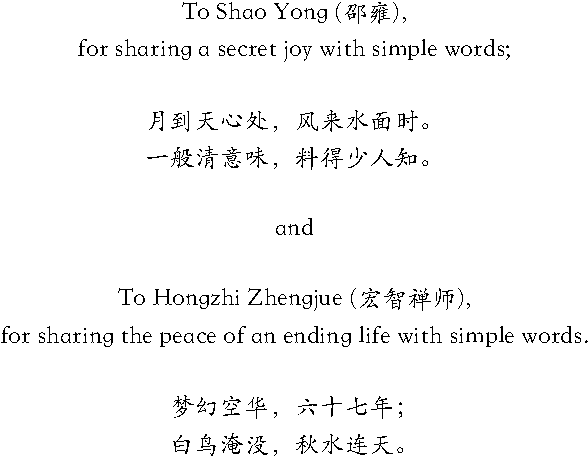
\includegraphics{images/dedication.pdf}
\end{center}

\setlength{\abovedisplayskip}{-5pt}
\setlength{\abovedisplayshortskip}{-5pt}

{
\setcounter{tocdepth}{1}
\tableofcontents
}
\hypertarget{prefuxe1cio}{%
\chapter*{Prefácio}\label{prefuxe1cio}}
\addcontentsline{toc}{chapter}{Prefácio}

Esta página serviu para estudo e prática com o pacote R Bookdown e contém a solução encontrada por mim para os exercícios propostos no livro R para Data Sciente, de Hadley Wickham e Garret Grolemund, publicado no Brasil em 2019 pela Alta Books Editora \citep{wickham2019}.

Por se tratar de um produto construído durante o processo de aprendizagem, o conteúdo pode conter erros, tanto no texto em si, como na lógica utilizada para solução dos exercícios.

Dúvidas ou sugestões de melhoria podem ser encaminhadas para o e-mail \emph{\href{mailto:jeidsan.pereira@gmail.com}{\nolinkurl{jeidsan.pereira@gmail.com}}}.

\hypertarget{penduxeancias}{%
\section*{Pendências}\label{penduxeancias}}
\addcontentsline{toc}{section}{Pendências}

\begin{itemize}
\tightlist
\item
  No PDF, o prefácio está sendo exibido duas vezes no sumário;
\item
  \protect\hyperlink{exr1-7-4}{Exercício 1.7.4};
\item
  \protect\hyperlink{exr2-3-3}{Exercício 2.3.3};
\item
\end{itemize}

\mainmatter

\hypertarget{part-explorar}{%
\part{Explorar}\label{part-explorar}}

\hypertarget{visualizauxe7uxe3o-de-dados-com-ggplot2}{%
\chapter{\texorpdfstring{Visualização de dados com \texttt{ggplot2}}{Visualização de dados com ggplot2}}\label{visualizauxe7uxe3o-de-dados-com-ggplot2}}

Para a correta execução dos códigos desse capítulo, utilizaremos algumas configurações específicas.

Inicialmente, precisaremos carregar o pacote \texttt{nycflights13}, que contém os dados de todos os voos da cidade de Nova York em 2013.

\begin{Shaded}
\begin{Highlighting}[]
\FunctionTok{library}\NormalTok{(nycflights13)}
\FunctionTok{library}\NormalTok{(gridExtra)}
\end{Highlighting}
\end{Shaded}

\begin{verbatim}
## 
## Attaching package: 'gridExtra'
\end{verbatim}

\begin{verbatim}
## The following object is masked from 'package:dplyr':
## 
##     combine
\end{verbatim}

\hypertarget{introduuxe7uxe3o}{%
\section{Introdução}\label{introduuxe7uxe3o}}

Não temos exercícios nesta seção.

\hypertarget{primeiros-passos}{%
\section{Primeiros passos}\label{primeiros-passos}}

\hypertarget{exr1-2-1}{%
\subsection*{Exercício 1.2.1}\label{exr1-2-1}}
\addcontentsline{toc}{subsection}{Exercício 1.2.1}

Execute \texttt{ggplot(data=mpg);}. O que você vê?

\begin{solution}
\leavevmode

\begin{Shaded}
\begin{Highlighting}[]
\FunctionTok{ggplot}\NormalTok{(}\AttributeTok{data=}\NormalTok{mpg) }\SpecialCharTok{+}
\NormalTok{    tema}
\end{Highlighting}
\end{Shaded}


\includegraphics{r4ds_files/figure-latex/unnamed-chunk-3-1.pdf}

É exibido um quadro em branco. Este quadro contém o sistema de coordenadas sobre o qual serão desenhados os grpaficos que pretendemos exibir.

\end{solution}

\hypertarget{exr1-2-2}{%
\subsection*{Exercício 1.2.2}\label{exr1-2-2}}
\addcontentsline{toc}{subsection}{Exercício 1.2.2}

Quantas linhas existem em \texttt{mtcars}? Quantas colunas?

\begin{solution}
\leavevmode

\begin{Shaded}
\begin{Highlighting}[]
\FunctionTok{dim}\NormalTok{(mtcars)}
\end{Highlighting}
\end{Shaded}

\begin{verbatim}
## [1] 32 11
\end{verbatim}

R.: Existem 32 linhas e 11 colunas.

\end{solution}

\hypertarget{exr1-2-3}{%
\subsection*{Exercício 1.2.3}\label{exr1-2-3}}
\addcontentsline{toc}{subsection}{Exercício 1.2.3}

O que a variável \texttt{drv} descreve?

\begin{solution}
Executamos o comando \texttt{?mpg} no console no R e a página de ajuda foi aberta. Nela encontramos o significado de cada variável do conjunto de dados.

A varíável descreve o tipo de tração dos carros analisados, onde \texttt{f} significa tração dianteira, \texttt{r} significa tração traseira e \texttt{4} significa tração nas quatro rodas.
\end{solution}

\hypertarget{ex1-2-4}{%
\subsection*{Exercício 1.2.4}\label{ex1-2-4}}
\addcontentsline{toc}{subsection}{Exercício 1.2.4}

Faça um gráfico de dispersão de \texttt{hwy} \emph{versus} \texttt{cyl}.

\begin{solution}
\leavevmode

\begin{Shaded}
\begin{Highlighting}[]
\FunctionTok{ggplot}\NormalTok{(}\AttributeTok{data =}\NormalTok{ mpg) }\SpecialCharTok{+}
    \FunctionTok{geom\_point}\NormalTok{(}\AttributeTok{mapping =} \FunctionTok{aes}\NormalTok{(}\AttributeTok{x =}\NormalTok{ hwy, }\AttributeTok{y =}\NormalTok{ cyl)) }\SpecialCharTok{+}
\NormalTok{    tema}
\end{Highlighting}
\end{Shaded}

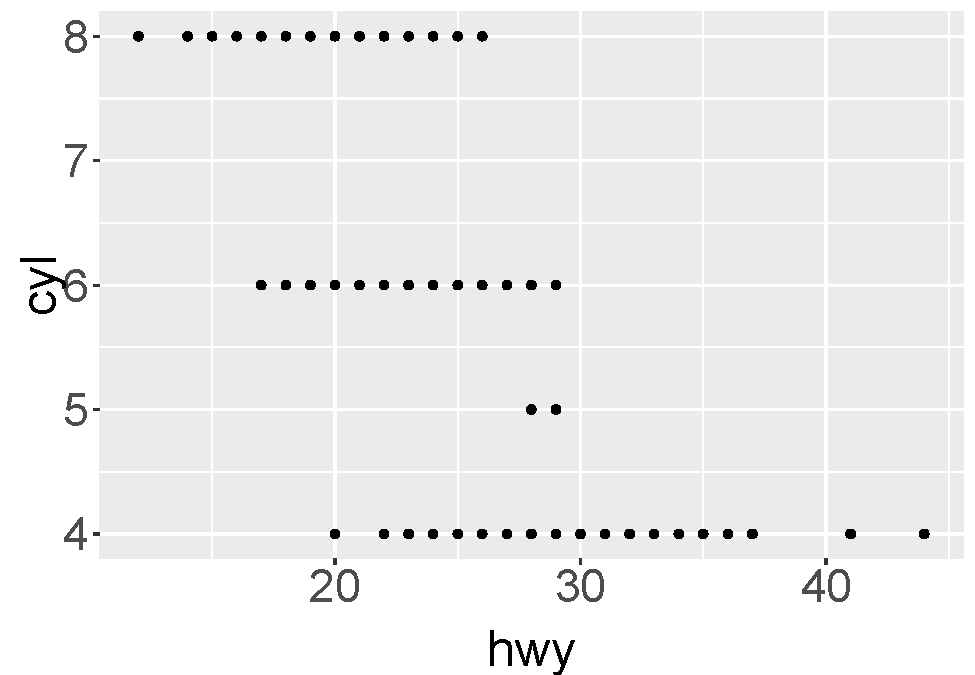
\includegraphics{r4ds_files/figure-latex/unnamed-chunk-5-1.pdf}

\end{solution}

\hypertarget{exr1-2-5}{%
\subsection*{Exercício 1.2.5}\label{exr1-2-5}}
\addcontentsline{toc}{subsection}{Exercício 1.2.5}

O que acontece se você fizer um gráfico de dispersão de \texttt{class} \emph{versus} \texttt{drv}? Por que esse gráfico não é útil?

\begin{solution}
\leavevmode

\begin{Shaded}
\begin{Highlighting}[]
\FunctionTok{ggplot}\NormalTok{(}\AttributeTok{data =}\NormalTok{ mpg) }\SpecialCharTok{+}
    \FunctionTok{geom\_point}\NormalTok{(}\AttributeTok{mapping =} \FunctionTok{aes}\NormalTok{(}\AttributeTok{x =}\NormalTok{ drv, }\AttributeTok{y =}\NormalTok{ class)) }\SpecialCharTok{+}
\NormalTok{    tema}
\end{Highlighting}
\end{Shaded}

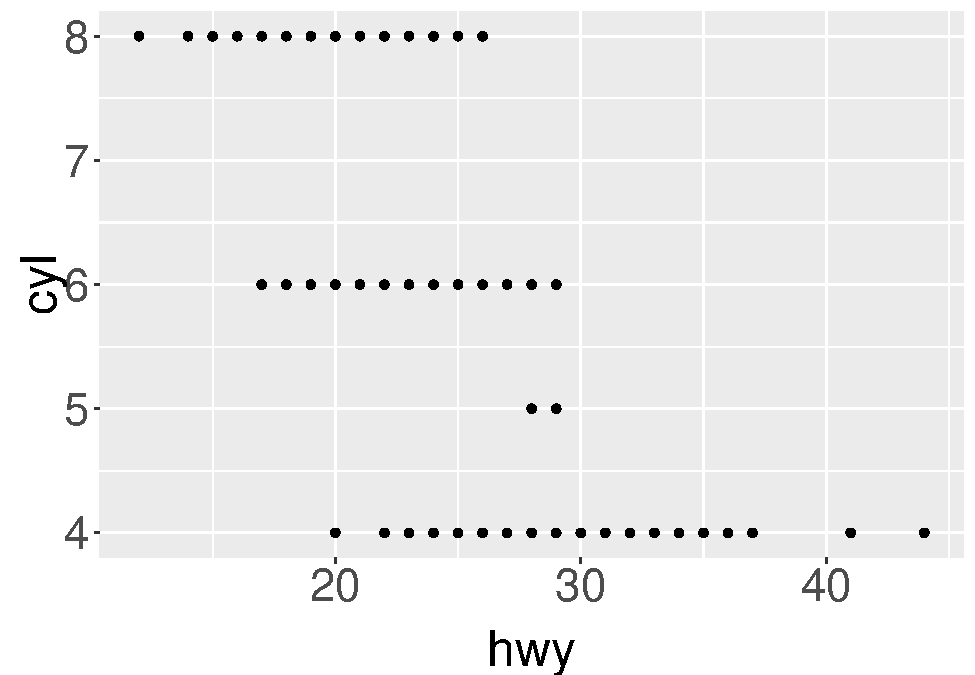
\includegraphics{r4ds_files/figure-latex/unnamed-chunk-6-1.pdf}

Apesar de serem exibidos dados no gráfico, nenhuma informação substancial é extraída, uma vez que o tipo de tração não está (a princípio) relacionado com a categoria do carro. Outro fator que torno o gráfico pouco informativo é que há, por exemplo, diversas SUVs com tração nas 4 rodas, contudo os valores ficam sobrepostos no gráfico, não dando dimensão do quanto de dados temos.

Abaixo seguem duas opções de como trazer mais informação ao gráfico:

\begin{itemize}
\tightlist
\item
  a primeira opção adiciona um ruído aos dados (\texttt{position\ =\ jitter} ou \texttt{geom\_jitter()}) de modo que não haja sobreposição;
\end{itemize}

\begin{Shaded}
\begin{Highlighting}[]
\FunctionTok{ggplot}\NormalTok{(}\AttributeTok{data =}\NormalTok{ mpg) }\SpecialCharTok{+}
    \FunctionTok{geom\_point}\NormalTok{(}\AttributeTok{mapping =} \FunctionTok{aes}\NormalTok{(}\AttributeTok{x =}\NormalTok{ drv, }\AttributeTok{y =}\NormalTok{ class), }\AttributeTok{position =} \StringTok{"jitter"}\NormalTok{) }\SpecialCharTok{+}
\NormalTok{    tema}
\end{Highlighting}
\end{Shaded}

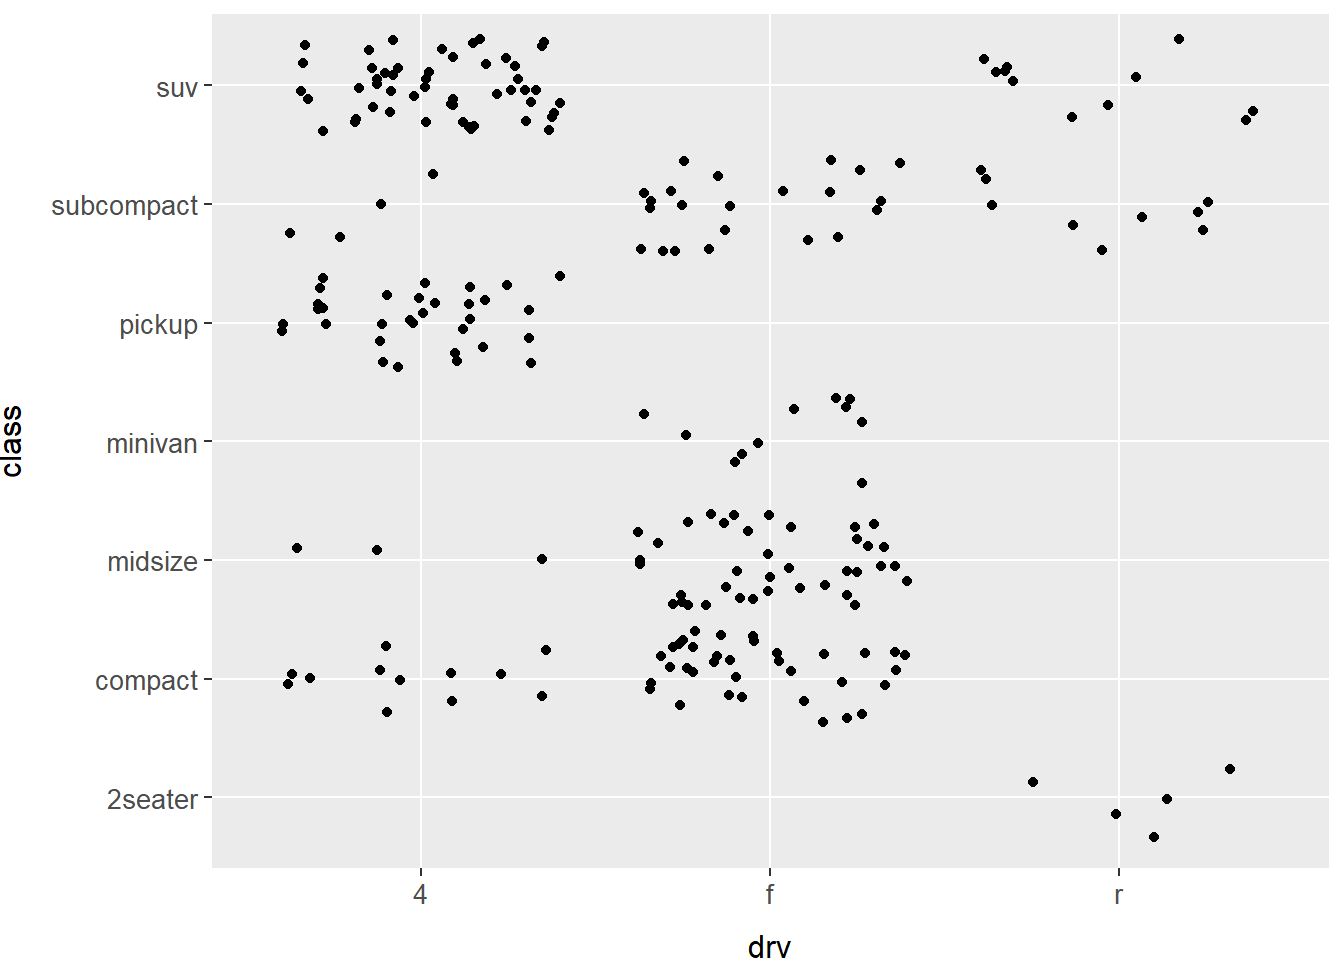
\includegraphics{r4ds_files/figure-latex/unnamed-chunk-7-1.pdf}

\begin{itemize}
\tightlist
\item
  a segunda opção, bem mais avançada, adiciona uma estética de \texttt{size} considerando a quantidade de registros.
\end{itemize}

\begin{Shaded}
\begin{Highlighting}[]
\NormalTok{mpg }\SpecialCharTok{\%\textgreater{}\%}
    \FunctionTok{group\_by}\NormalTok{(class, drv) }\SpecialCharTok{\%\textgreater{}\%}
    \FunctionTok{summarize}\NormalTok{(}\AttributeTok{count =} \FunctionTok{n}\NormalTok{()) }\SpecialCharTok{\%\textgreater{}\%}
    \FunctionTok{ggplot}\NormalTok{(}\AttributeTok{mapping =} \FunctionTok{aes}\NormalTok{(}\AttributeTok{x =}\NormalTok{ drv, }\AttributeTok{y =}\NormalTok{ class, }\AttributeTok{size =}\NormalTok{ count)) }\SpecialCharTok{+}
        \FunctionTok{geom\_point}\NormalTok{() }\SpecialCharTok{+}
\NormalTok{        tema}
\end{Highlighting}
\end{Shaded}

\begin{verbatim}
## `summarise()` has grouped output by 'class'. You can override using the
## `.groups` argument.
\end{verbatim}

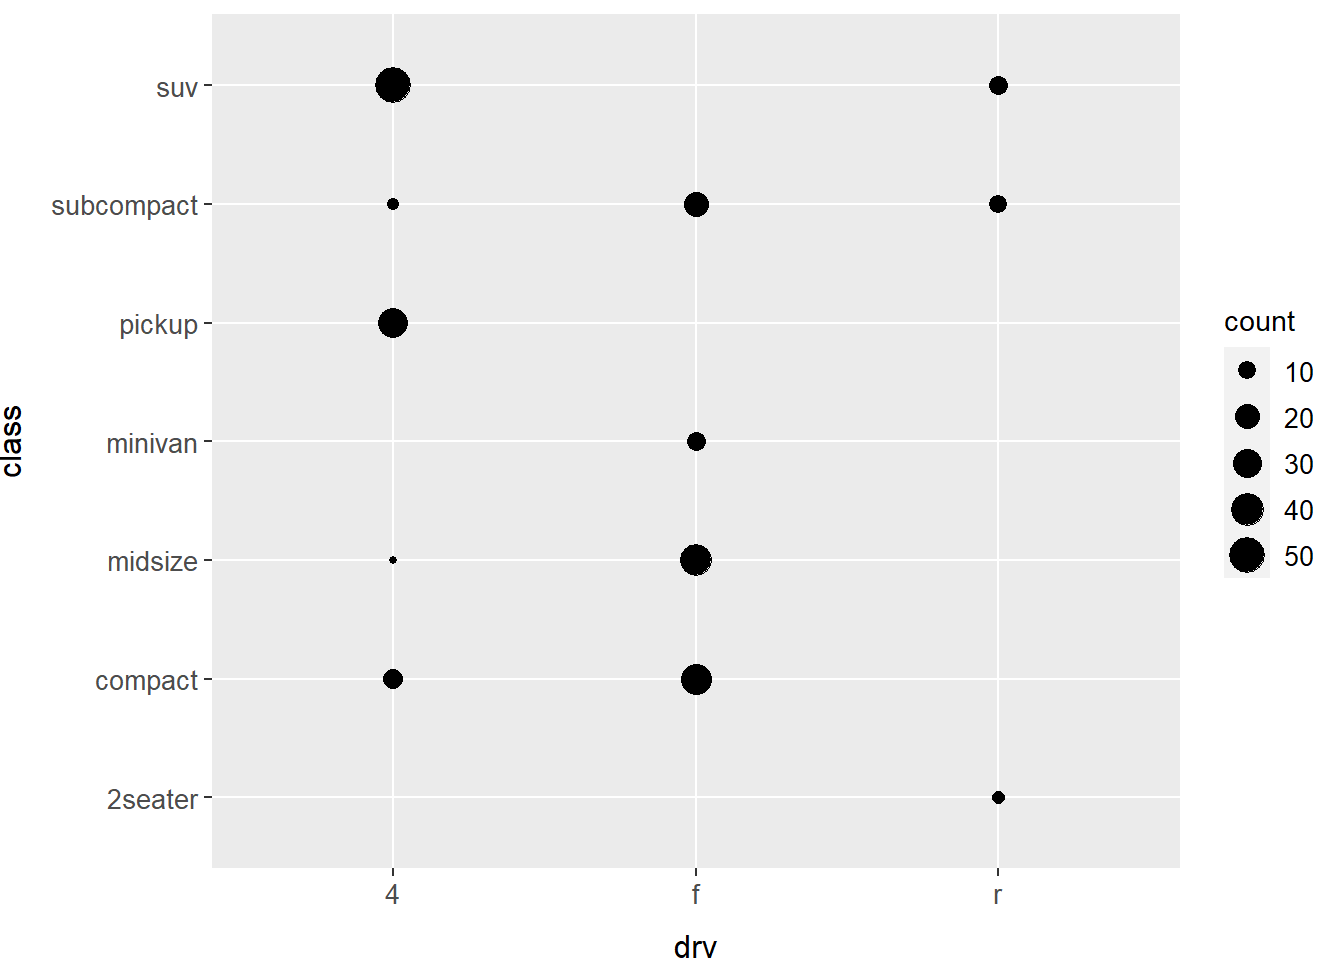
\includegraphics{r4ds_files/figure-latex/unnamed-chunk-8-1.pdf}

\end{solution}

\hypertarget{mapeamentos-estuxe9ticos}{%
\section{Mapeamentos estéticos}\label{mapeamentos-estuxe9ticos}}

\hypertarget{exr1-3-1}{%
\subsection*{Exercício 1.3.1}\label{exr1-3-1}}
\addcontentsline{toc}{subsection}{Exercício 1.3.1}

O que há de errado com este código? Por que os pontos não estão azuis?

\begin{Shaded}
\begin{Highlighting}[]
\FunctionTok{ggplot}\NormalTok{(}\AttributeTok{data =}\NormalTok{ mpg) }\SpecialCharTok{+}
    \FunctionTok{geom\_point}\NormalTok{(}\AttributeTok{mapping =} \FunctionTok{aes}\NormalTok{(}\AttributeTok{x =}\NormalTok{ displ, }\AttributeTok{y =}\NormalTok{ hwy, }\AttributeTok{color =} \StringTok{"blue"}\NormalTok{)) }\SpecialCharTok{+}
\NormalTok{    tema}
\end{Highlighting}
\end{Shaded}

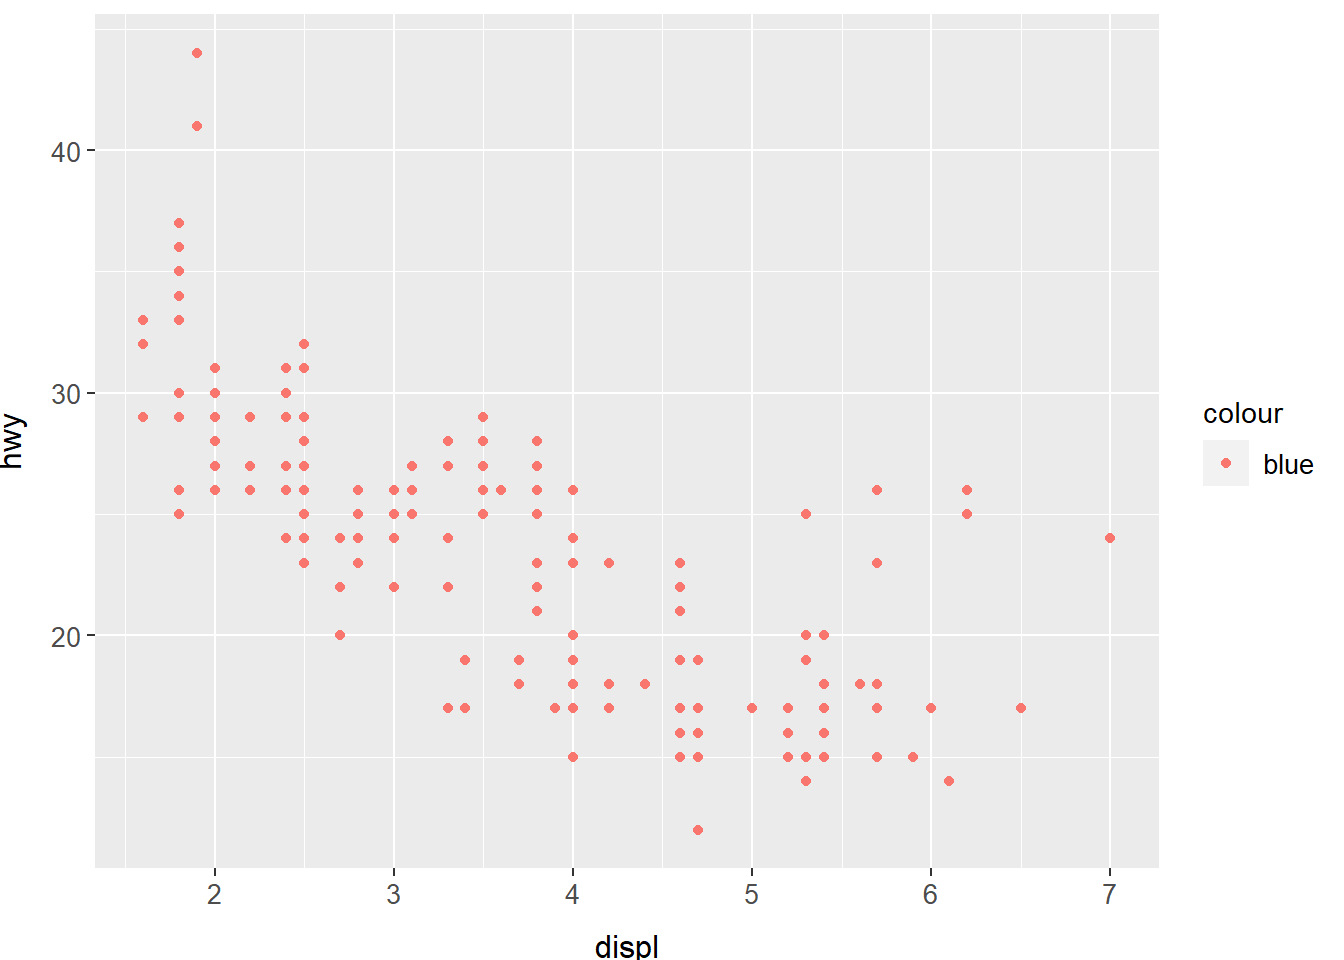
\includegraphics{r4ds_files/figure-latex/unnamed-chunk-9-1.pdf}

\begin{solution}
Ao invés de atribuir uma cor aos elementos de \texttt{geom\_point}, o atributo \texttt{color} foi passado como uma estética. O gráfico deveria ser construído da seguinte maneira:

\begin{Shaded}
\begin{Highlighting}[]
\FunctionTok{ggplot}\NormalTok{(}\AttributeTok{data =}\NormalTok{ mpg) }\SpecialCharTok{+}
    \FunctionTok{geom\_point}\NormalTok{(}\AttributeTok{mapping =} \FunctionTok{aes}\NormalTok{(}\AttributeTok{x =}\NormalTok{ displ, }\AttributeTok{y =}\NormalTok{ hwy), }\AttributeTok{color =} \StringTok{"blue"}\NormalTok{) }\SpecialCharTok{+}
\NormalTok{    tema}
\end{Highlighting}
\end{Shaded}

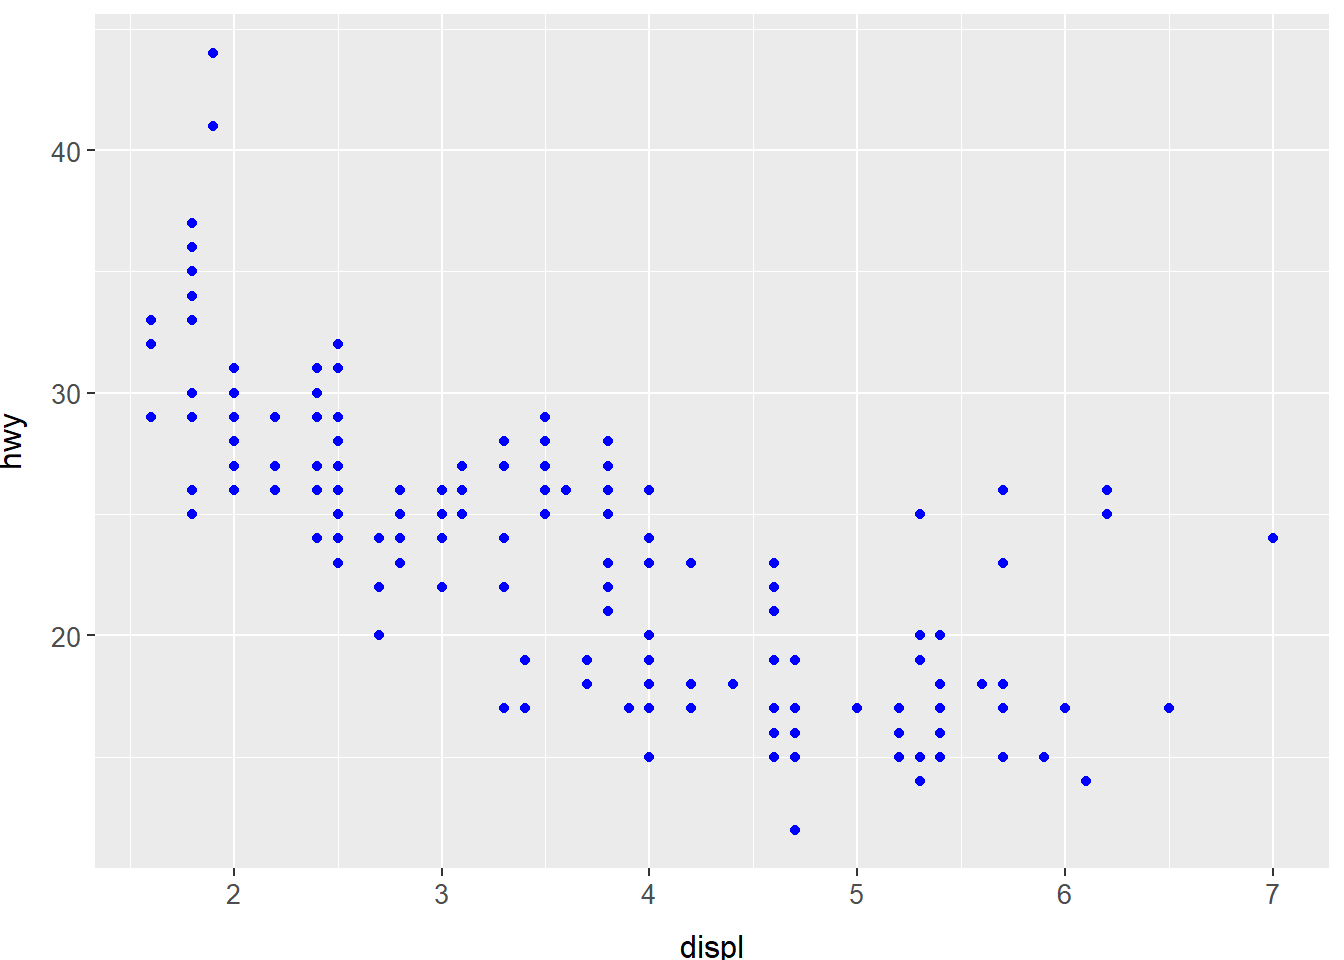
\includegraphics{r4ds_files/figure-latex/unnamed-chunk-10-1.pdf}
\end{solution}

\hypertarget{exr1-3-2}{%
\subsection*{Exercício 1.3.2}\label{exr1-3-2}}
\addcontentsline{toc}{subsection}{Exercício 1.3.2}

Quais variáveis em \texttt{mpg} são categóricas? Quais variáveis são contínuas? Como você pode ver essa informação quando executa \texttt{mpg}?

\begin{solution}
Usando \texttt{?mpg} vemos que as variáveis categóricas são: \texttt{manufacturer}, \texttt{model}, \texttt{trans}, \texttt{drv}, \texttt{fl} e \texttt{class}. As variáveis contínuas são: \texttt{displ}, \texttt{cty}, \texttt{hwy}.
\end{solution}

\hypertarget{exr1-3-3}{%
\subsection*{Exercício 1.3.3}\label{exr1-3-3}}
\addcontentsline{toc}{subsection}{Exercício 1.3.3}

Mapeie uma variável contínua para \texttt{color}, \texttt{size} e \texttt{shape}. Como essas estéticas se comportam de maneira diferente para variáveis categóricas e contínuas?

\begin{solution}
\leavevmode

\begin{Shaded}
\begin{Highlighting}[]
\FunctionTok{ggplot}\NormalTok{(}\AttributeTok{data =}\NormalTok{ mpg) }\SpecialCharTok{+}
    \FunctionTok{geom\_point}\NormalTok{(}\AttributeTok{mapping =} \FunctionTok{aes}\NormalTok{(}\AttributeTok{x =}\NormalTok{ displ, }\AttributeTok{y =}\NormalTok{ hwy, }\AttributeTok{color =}\NormalTok{ displ)) }\SpecialCharTok{+}
\NormalTok{    tema}
\end{Highlighting}
\end{Shaded}

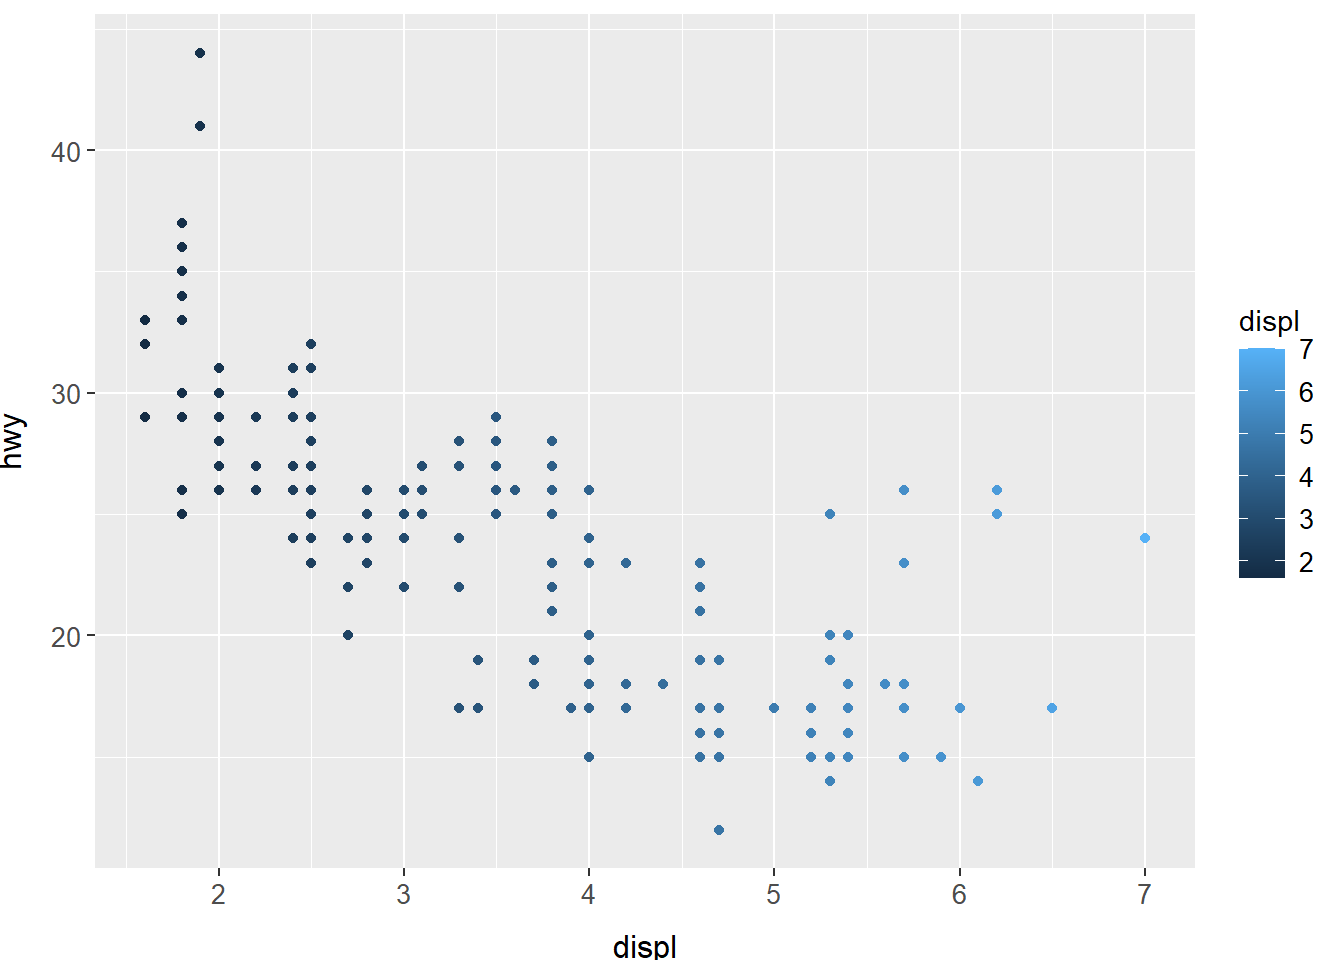
\includegraphics{r4ds_files/figure-latex/unnamed-chunk-11-1.pdf}

\begin{Shaded}
\begin{Highlighting}[]
\FunctionTok{ggplot}\NormalTok{(}\AttributeTok{data =}\NormalTok{ mpg) }\SpecialCharTok{+}
    \FunctionTok{geom\_point}\NormalTok{(}\AttributeTok{mapping =} \FunctionTok{aes}\NormalTok{(}\AttributeTok{x =}\NormalTok{ displ, }\AttributeTok{y =}\NormalTok{ hwy, }\AttributeTok{size =}\NormalTok{ displ)) }\SpecialCharTok{+}
\NormalTok{    tema}
\end{Highlighting}
\end{Shaded}

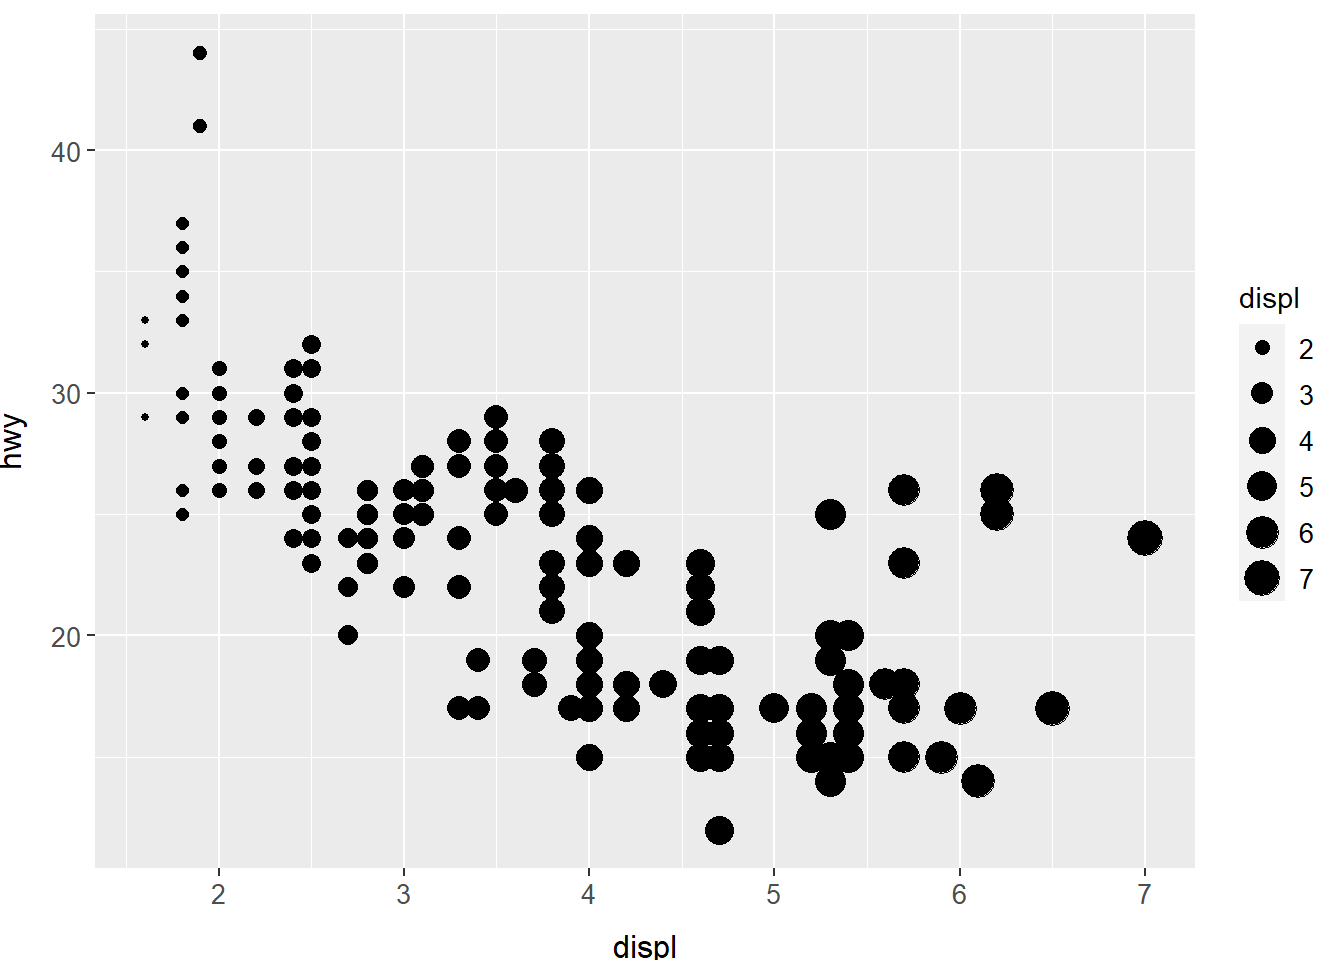
\includegraphics{r4ds_files/figure-latex/unnamed-chunk-12-1.pdf}

\begin{Shaded}
\begin{Highlighting}[]
\FunctionTok{ggplot}\NormalTok{(}\AttributeTok{data =}\NormalTok{ mpg) }\SpecialCharTok{+}
    \FunctionTok{geom\_point}\NormalTok{(}\AttributeTok{mapping =} \FunctionTok{aes}\NormalTok{(}\AttributeTok{x =}\NormalTok{ displ, }\AttributeTok{y =}\NormalTok{ hwy, }\AttributeTok{shape =}\NormalTok{ displ)) }\SpecialCharTok{+}
\NormalTok{    tema}
\end{Highlighting}
\end{Shaded}

\begin{verbatim}
## Error in `geom_point()`:
## ! Problem while computing aesthetics.
## i Error occurred in the 1st layer.
## Caused by error in `scale_f()`:
## ! A continuous variable cannot be mapped to the shape aesthetic
## i choose a different aesthetic or use `scale_shape_binned()`
\end{verbatim}

Quando possível, a biblioteca \emph{ggplot} apesenta a estética em um gradiente, como em color e size. Porém, nem sempre isso é possível, como vemos em \texttt{shape}, que só pode ser utilizada com variáveis discretas ou categóricas.

\end{solution}

\hypertarget{exr1-3-4}{%
\subsection*{Exercício 1.3.4}\label{exr1-3-4}}
\addcontentsline{toc}{subsection}{Exercício 1.3.4}

O que acontece se você mapear a mesma variável a várias estéticas?

\begin{solution}
\leavevmode

\begin{Shaded}
\begin{Highlighting}[]
\FunctionTok{ggplot}\NormalTok{(}\AttributeTok{data =}\NormalTok{ mpg) }\SpecialCharTok{+}
    \FunctionTok{geom\_point}\NormalTok{(}\AttributeTok{mapping =} \FunctionTok{aes}\NormalTok{(}\AttributeTok{x =}\NormalTok{ displ, }\AttributeTok{y =}\NormalTok{ hwy, }\AttributeTok{size =}\NormalTok{ class, }\AttributeTok{color =}\NormalTok{ class, }\AttributeTok{shape =}\NormalTok{ class)) }\SpecialCharTok{+}
\NormalTok{    tema}
\end{Highlighting}
\end{Shaded}

\begin{verbatim}
## Warning: Using size for a discrete variable is not advised.
\end{verbatim}

\begin{verbatim}
## Warning: The shape palette can deal with a maximum of 6 discrete values because
## more than 6 becomes difficult to discriminate; you have 7. Consider
## specifying shapes manually if you must have them.
\end{verbatim}

\begin{verbatim}
## Warning: Removed 62 rows containing missing values (`geom_point()`).
\end{verbatim}

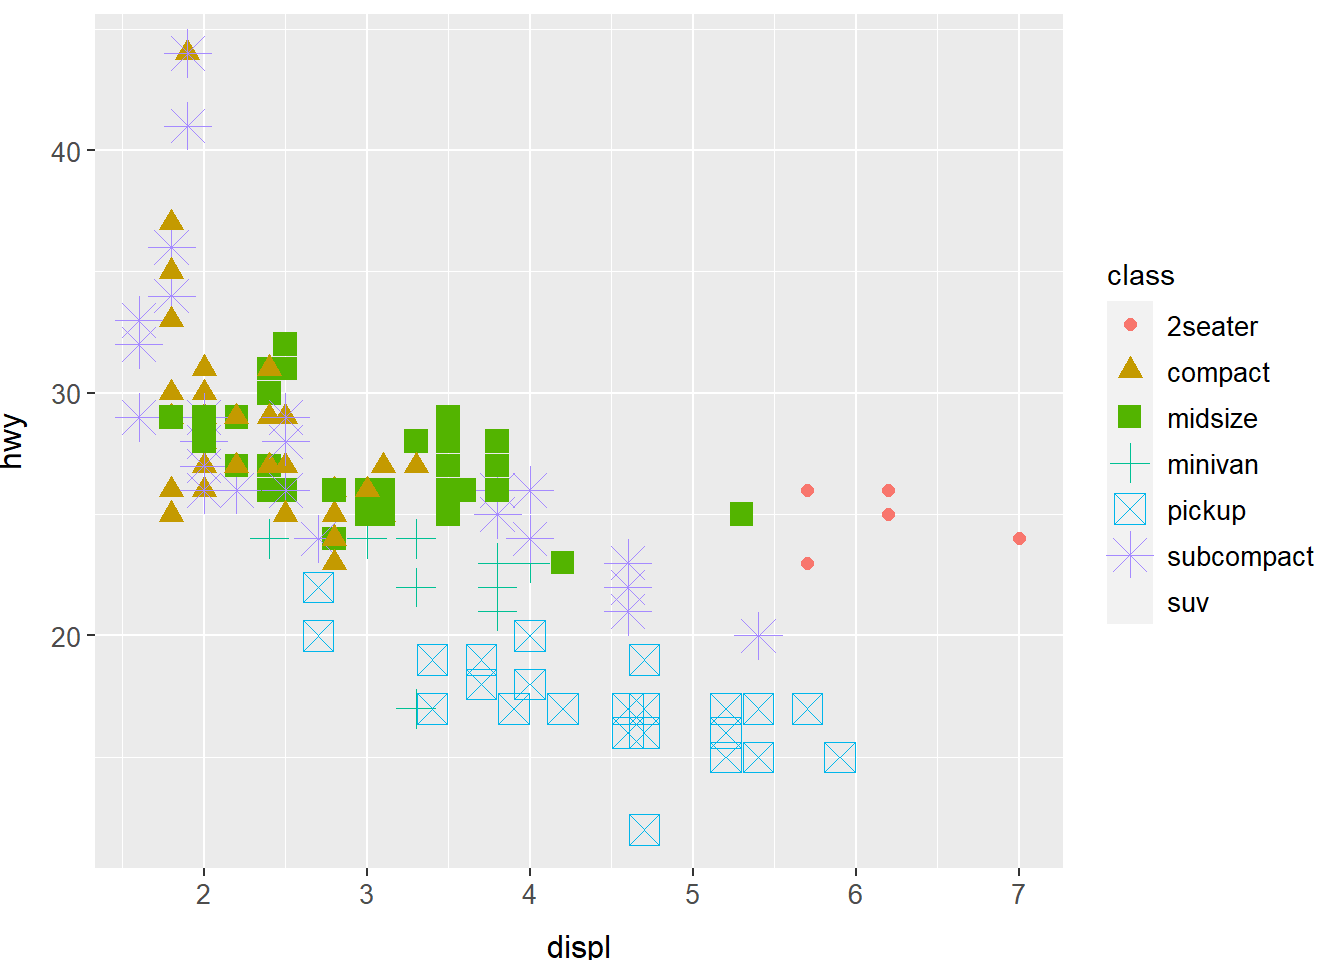
\includegraphics{r4ds_files/figure-latex/unnamed-chunk-14-1.pdf}

Os valores da variável serão representados de modo a atender todas as estéticas simultaneamente, por exemplo, no gráfico acima é dada uma cor, um formato e um tamanho específicos para cada classe de veículo. Os veículos de dois lugares são exibidos como um disco rosa pequeno.

\end{solution}

\hypertarget{exr1-3-5}{%
\subsection*{Exercício 1.3.5}\label{exr1-3-5}}
\addcontentsline{toc}{subsection}{Exercício 1.3.5}

O que a estética \texttt{stroke} faz? com que formas ela trabalha?

\begin{solution}
\leavevmode

\begin{Shaded}
\begin{Highlighting}[]
\FunctionTok{ggplot}\NormalTok{(}\AttributeTok{data =}\NormalTok{ mpg) }\SpecialCharTok{+}
    \FunctionTok{geom\_point}\NormalTok{(}\AttributeTok{mapping =} \FunctionTok{aes}\NormalTok{(}\AttributeTok{x =}\NormalTok{ displ, }\AttributeTok{y =}\NormalTok{ hwy, }\AttributeTok{stroke =}\NormalTok{ displ)) }\SpecialCharTok{+}
\NormalTok{    tema}
\end{Highlighting}
\end{Shaded}

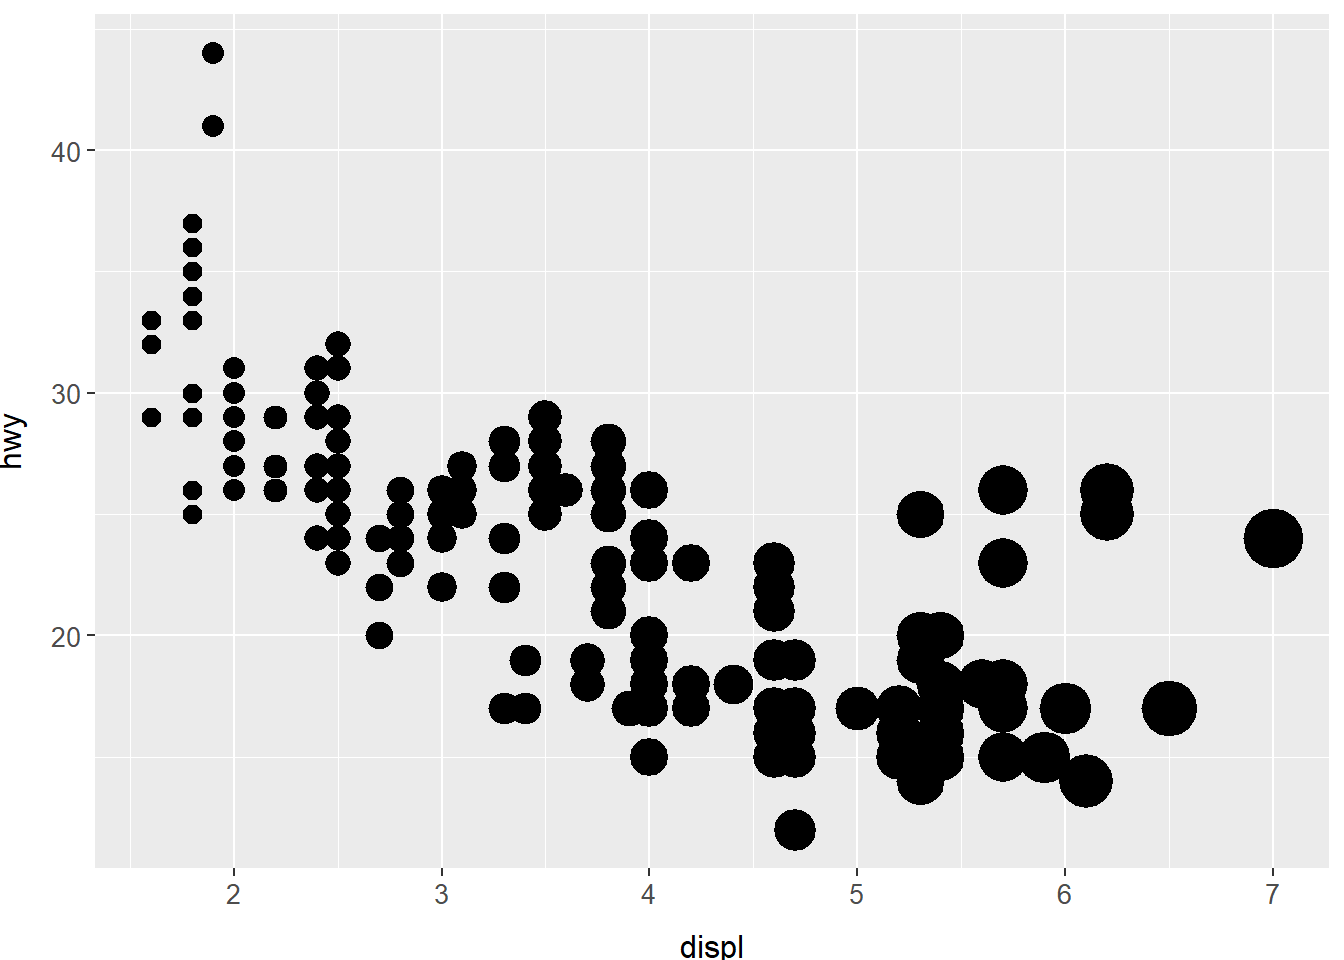
\includegraphics{r4ds_files/figure-latex/unnamed-chunk-15-1.pdf}

A estética \texttt{stroke} controla a espessura do ponto ou elemento a ser representado.

\end{solution}

\hypertarget{exr1-3-6}{%
\subsection*{Exercício 1.3.6}\label{exr1-3-6}}
\addcontentsline{toc}{subsection}{Exercício 1.3.6}

O que acontece se você mapear uma estética a algo diferente de um nome de variável, como \texttt{aes(color\ =\ displ\ \textless{}\ 5)}?

\begin{solution}
\leavevmode

\begin{Shaded}
\begin{Highlighting}[]
\FunctionTok{ggplot}\NormalTok{(}\AttributeTok{data =}\NormalTok{ mpg) }\SpecialCharTok{+}
    \FunctionTok{geom\_point}\NormalTok{(}\AttributeTok{mapping =} \FunctionTok{aes}\NormalTok{(}\AttributeTok{x =}\NormalTok{ displ, }\AttributeTok{y =}\NormalTok{ hwy, }\AttributeTok{color =}\NormalTok{ displ }\SpecialCharTok{\textless{}} \DecValTok{5}\NormalTok{)) }\SpecialCharTok{+}
\NormalTok{    tema}
\end{Highlighting}
\end{Shaded}

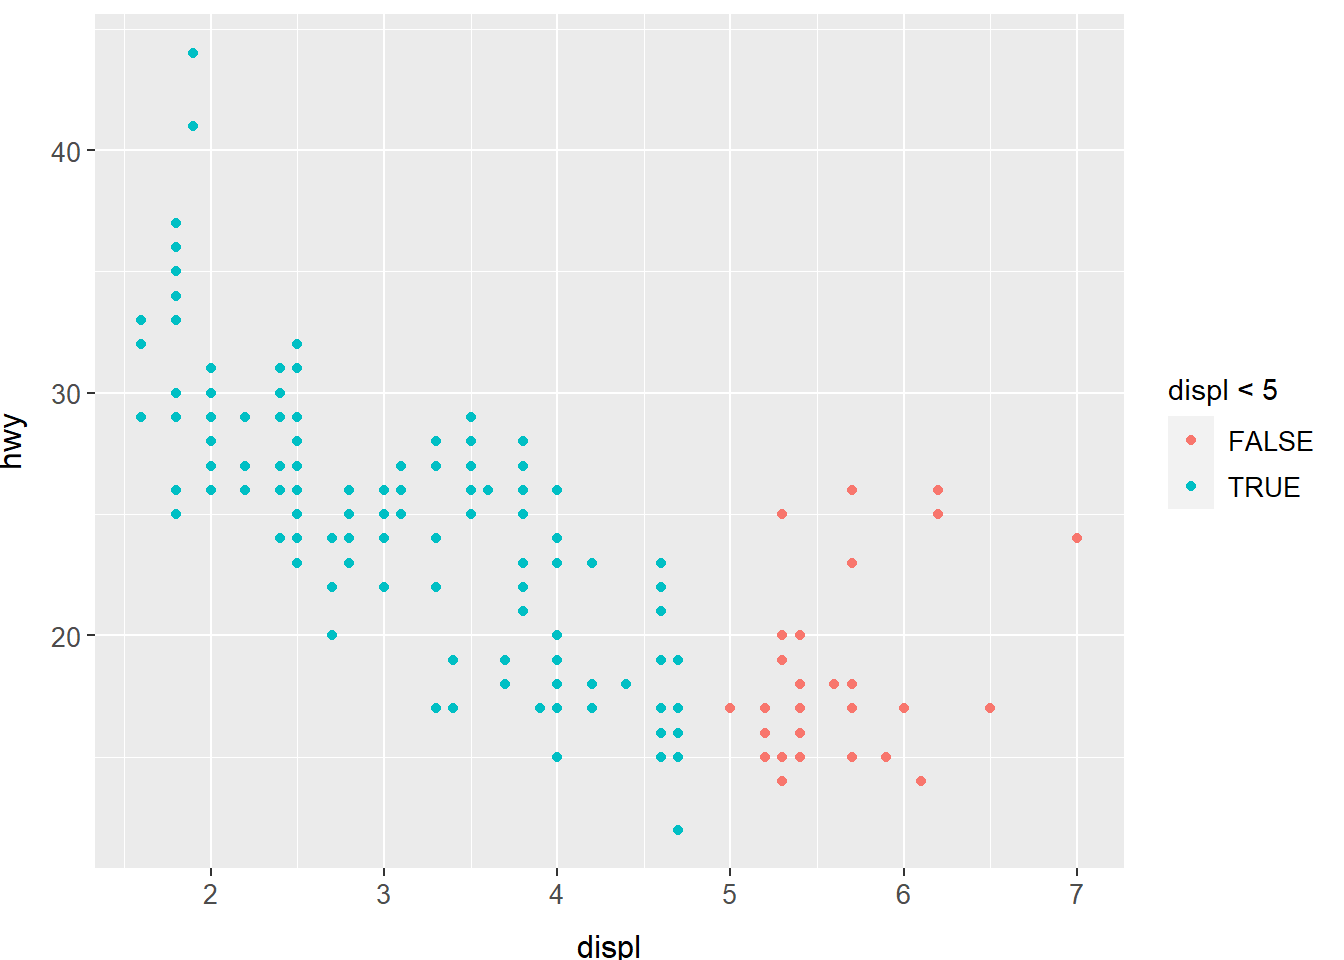
\includegraphics{r4ds_files/figure-latex/unnamed-chunk-16-1.pdf}

A expressão é avaliada para cada um dos valores da variável e o resultado é utilizado para plotagem da estética no gráfico.

\end{solution}

\hypertarget{problemas-comuns}{%
\section{Problemas comuns}\label{problemas-comuns}}

Não temos exercícios nessa seção.

\hypertarget{facetas}{%
\section{Facetas}\label{facetas}}

\hypertarget{exr1-5-1}{%
\subsection*{Exercício 1.5.1}\label{exr1-5-1}}
\addcontentsline{toc}{subsection}{Exercício 1.5.1}

O que acontece se você criar facetas em uma variável contínua?

\begin{solution}
\leavevmode

\begin{Shaded}
\begin{Highlighting}[]
\FunctionTok{ggplot}\NormalTok{(}\AttributeTok{data =}\NormalTok{ mpg) }\SpecialCharTok{+}
    \FunctionTok{geom\_point}\NormalTok{(}\AttributeTok{mapping =} \FunctionTok{aes}\NormalTok{(}\AttributeTok{x =}\NormalTok{ displ, }\AttributeTok{y =}\NormalTok{ hwy)) }\SpecialCharTok{+}
    \FunctionTok{facet\_wrap}\NormalTok{(. }\SpecialCharTok{\textasciitilde{}}\NormalTok{ displ) }\SpecialCharTok{+}
\NormalTok{    tema}
\end{Highlighting}
\end{Shaded}

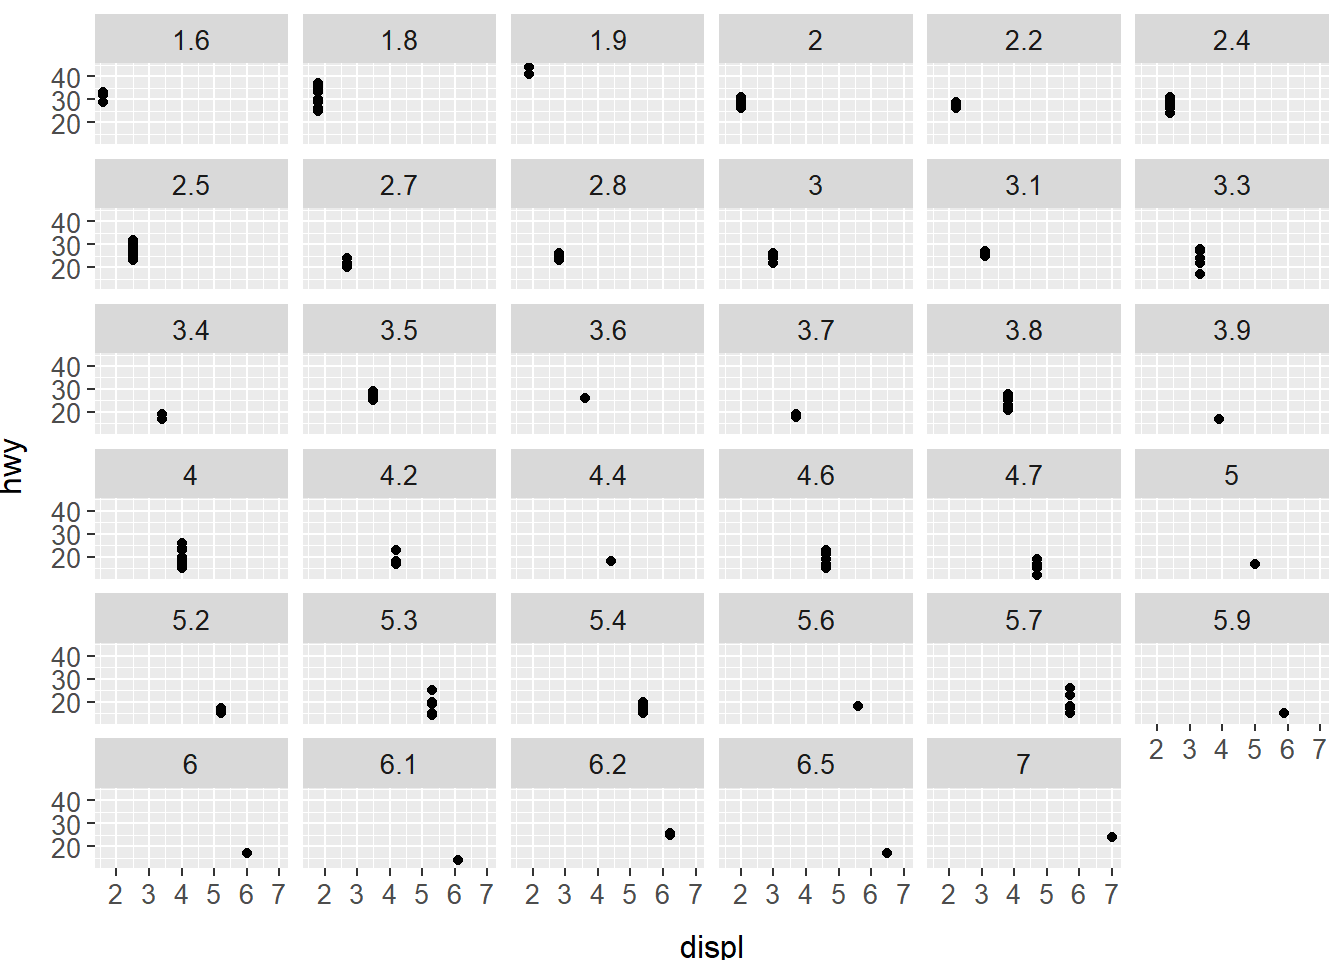
\includegraphics{r4ds_files/figure-latex/unnamed-chunk-17-1.pdf}

O \emph{ggplot} se encarrega de dividir o conjunto em classes e toma o ponto médio de cada classe para realizar a quebra em facetas.

\end{solution}

\hypertarget{exr1-5-2}{%
\subsection*{Exercício 1.5.2}\label{exr1-5-2}}
\addcontentsline{toc}{subsection}{Exercício 1.5.2}

O que significam as célula em branco em um gráfico com \texttt{facet\_grid(drv\ \textasciitilde{}\ cyl)}? Como elas se relacionam a este gráfico?

\begin{Shaded}
\begin{Highlighting}[]
\FunctionTok{ggplot}\NormalTok{(}\AttributeTok{data =}\NormalTok{ mpg) }\SpecialCharTok{+}
    \FunctionTok{geom\_point}\NormalTok{(}\AttributeTok{mapping =} \FunctionTok{aes}\NormalTok{(}\AttributeTok{x =}\NormalTok{ displ, }\AttributeTok{y =}\NormalTok{ hwy)) }\SpecialCharTok{+}
    \FunctionTok{facet\_grid}\NormalTok{(drv }\SpecialCharTok{\textasciitilde{}}\NormalTok{ cyl) }\SpecialCharTok{+}
\NormalTok{    tema}
\end{Highlighting}
\end{Shaded}

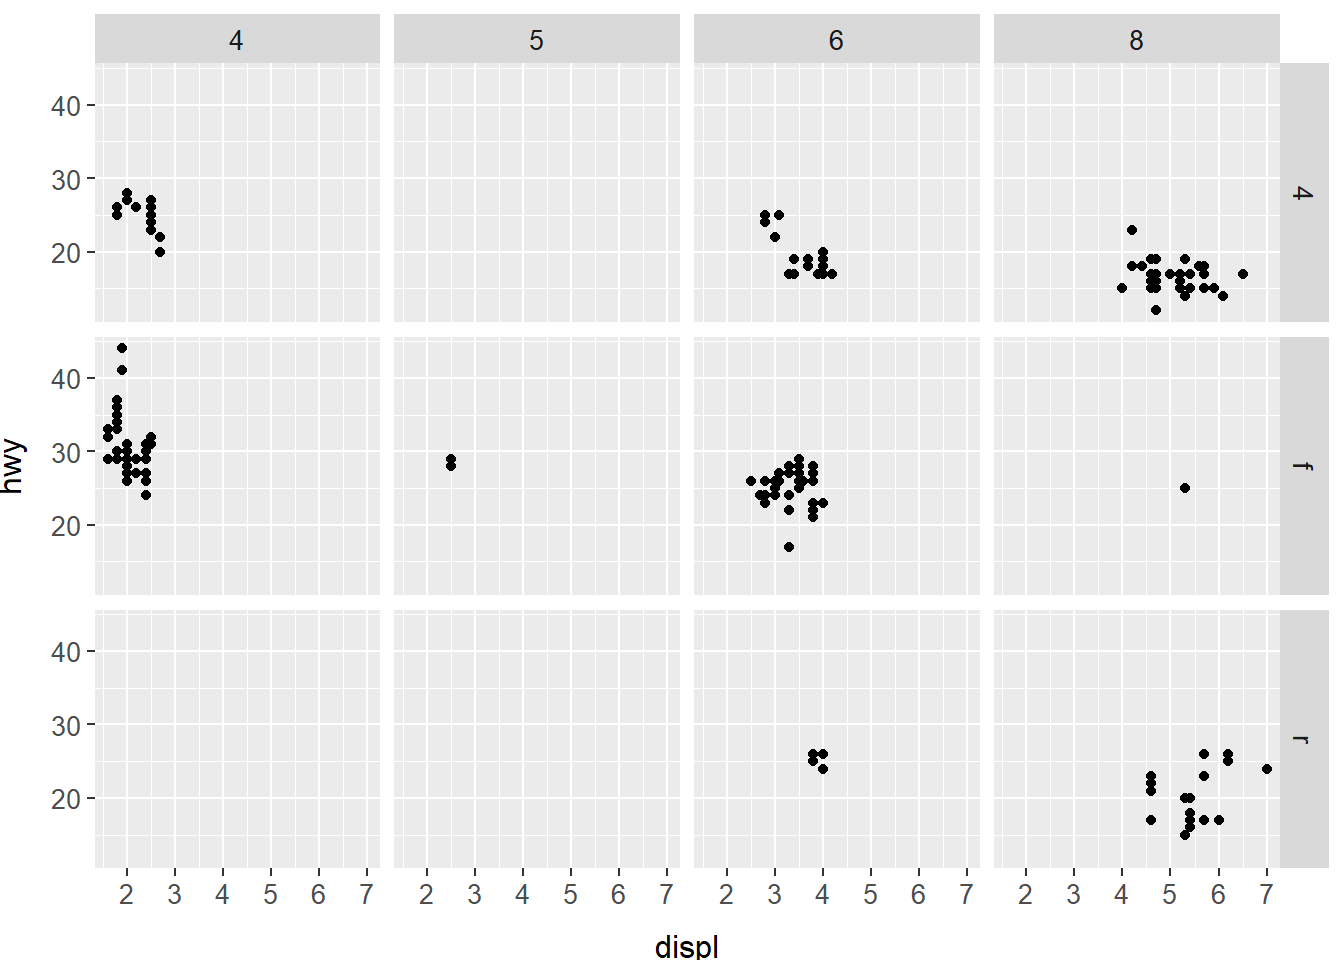
\includegraphics{r4ds_files/figure-latex/unnamed-chunk-18-1.pdf}

\begin{solution}
Significa que para aquela combinação de variáveis, não há nenhum valor observado. Por exemplo, não há nenhum veículo com 5 cilindros e tração nas quatro rodas.
\end{solution}

\hypertarget{exr1-5-3}{%
\subsection*{Exercício 1.5.3}\label{exr1-5-3}}
\addcontentsline{toc}{subsection}{Exercício 1.5.3}

Que gráficos o código a seguir faz? O que \texttt{.} faz?

\begin{Shaded}
\begin{Highlighting}[]
\FunctionTok{ggplot}\NormalTok{(}\AttributeTok{data =}\NormalTok{ mpg) }\SpecialCharTok{+}
    \FunctionTok{geom\_point}\NormalTok{(}\AttributeTok{mapping =} \FunctionTok{aes}\NormalTok{(}\AttributeTok{x =}\NormalTok{ displ, }\AttributeTok{y =}\NormalTok{ hwy)) }\SpecialCharTok{+}
    \FunctionTok{facet\_grid}\NormalTok{(drv }\SpecialCharTok{\textasciitilde{}}\NormalTok{ .) }\SpecialCharTok{+}
\NormalTok{    tema}
\end{Highlighting}
\end{Shaded}

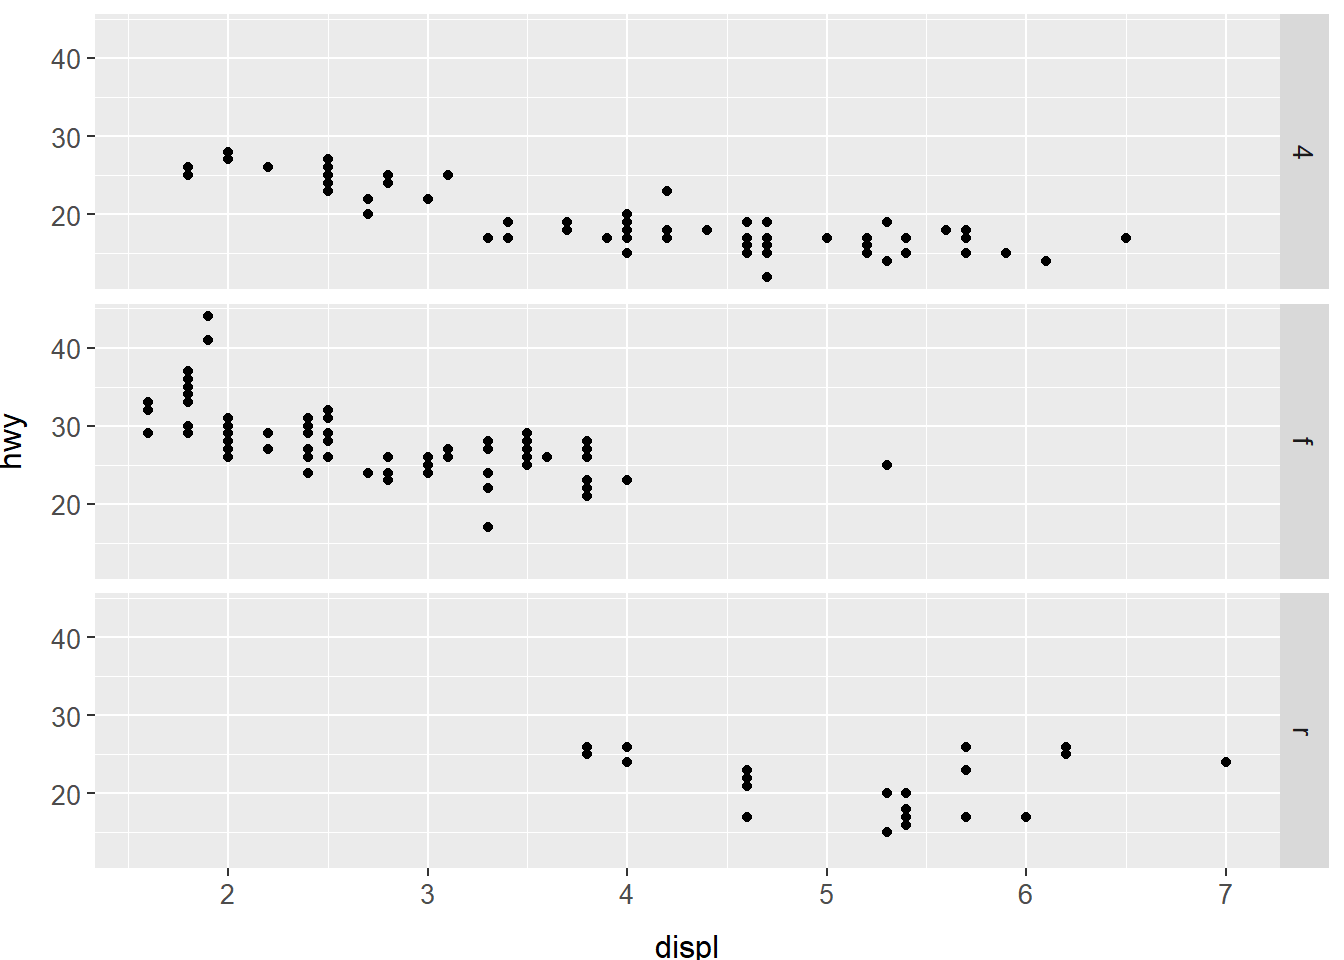
\includegraphics{r4ds_files/figure-latex/unnamed-chunk-19-1.pdf}

\begin{Shaded}
\begin{Highlighting}[]
\FunctionTok{ggplot}\NormalTok{(}\AttributeTok{data =}\NormalTok{ mpg) }\SpecialCharTok{+}
    \FunctionTok{geom\_point}\NormalTok{(}\AttributeTok{mapping =} \FunctionTok{aes}\NormalTok{(}\AttributeTok{x =}\NormalTok{ displ, }\AttributeTok{y =}\NormalTok{ hwy)) }\SpecialCharTok{+}
    \FunctionTok{facet\_grid}\NormalTok{(. }\SpecialCharTok{\textasciitilde{}}\NormalTok{ cyl) }\SpecialCharTok{+}
\NormalTok{    tema}
\end{Highlighting}
\end{Shaded}

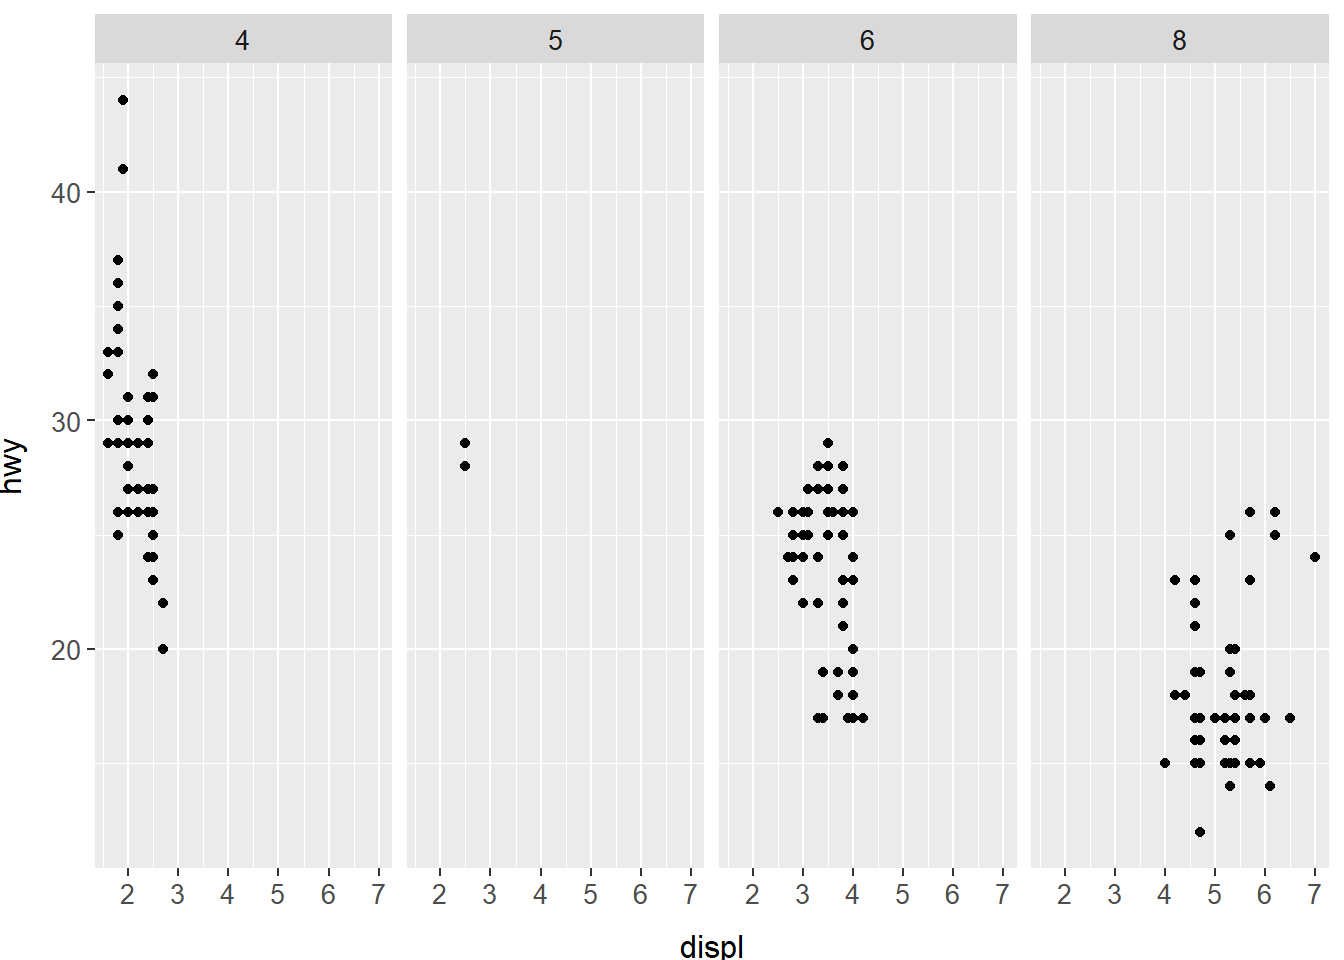
\includegraphics{r4ds_files/figure-latex/unnamed-chunk-20-1.pdf}

\begin{solution}
São gerados os gráficos de dispersão segregados pelas variáveis \texttt{drv} e \texttt{cyl}, respectivamente. O \texttt{.} indica que não queremos considerar nenhuma segregação naquela dimensão do \emph{grid} (linha ou coluna).
\end{solution}

\hypertarget{exr1-5-4}{%
\subsection*{Exercício 1.5.4}\label{exr1-5-4}}
\addcontentsline{toc}{subsection}{Exercício 1.5.4}

Pegue o primeiro gráfico em facetas dessa seção.

\begin{Shaded}
\begin{Highlighting}[]
\FunctionTok{ggplot}\NormalTok{(}\AttributeTok{data =}\NormalTok{ mpg) }\SpecialCharTok{+}
    \FunctionTok{geom\_point}\NormalTok{(}\AttributeTok{data =} \FunctionTok{transform}\NormalTok{(mpg, }\AttributeTok{class =} \ConstantTok{NULL}\NormalTok{), }\AttributeTok{mapping =} \FunctionTok{aes}\NormalTok{(}\AttributeTok{x =}\NormalTok{ displ, }\AttributeTok{y =}\NormalTok{ hwy), }\AttributeTok{color =} \StringTok{"gray80"}\NormalTok{) }\SpecialCharTok{+}
    \FunctionTok{geom\_point}\NormalTok{(}\AttributeTok{mapping =} \FunctionTok{aes}\NormalTok{(}\AttributeTok{x =}\NormalTok{ displ, }\AttributeTok{y =}\NormalTok{ hwy)) }\SpecialCharTok{+}
    \FunctionTok{facet\_wrap}\NormalTok{(}\SpecialCharTok{\textasciitilde{}}\NormalTok{ class, }\AttributeTok{nrow =} \DecValTok{2}\NormalTok{) }\SpecialCharTok{+}
\NormalTok{    tema}
\end{Highlighting}
\end{Shaded}

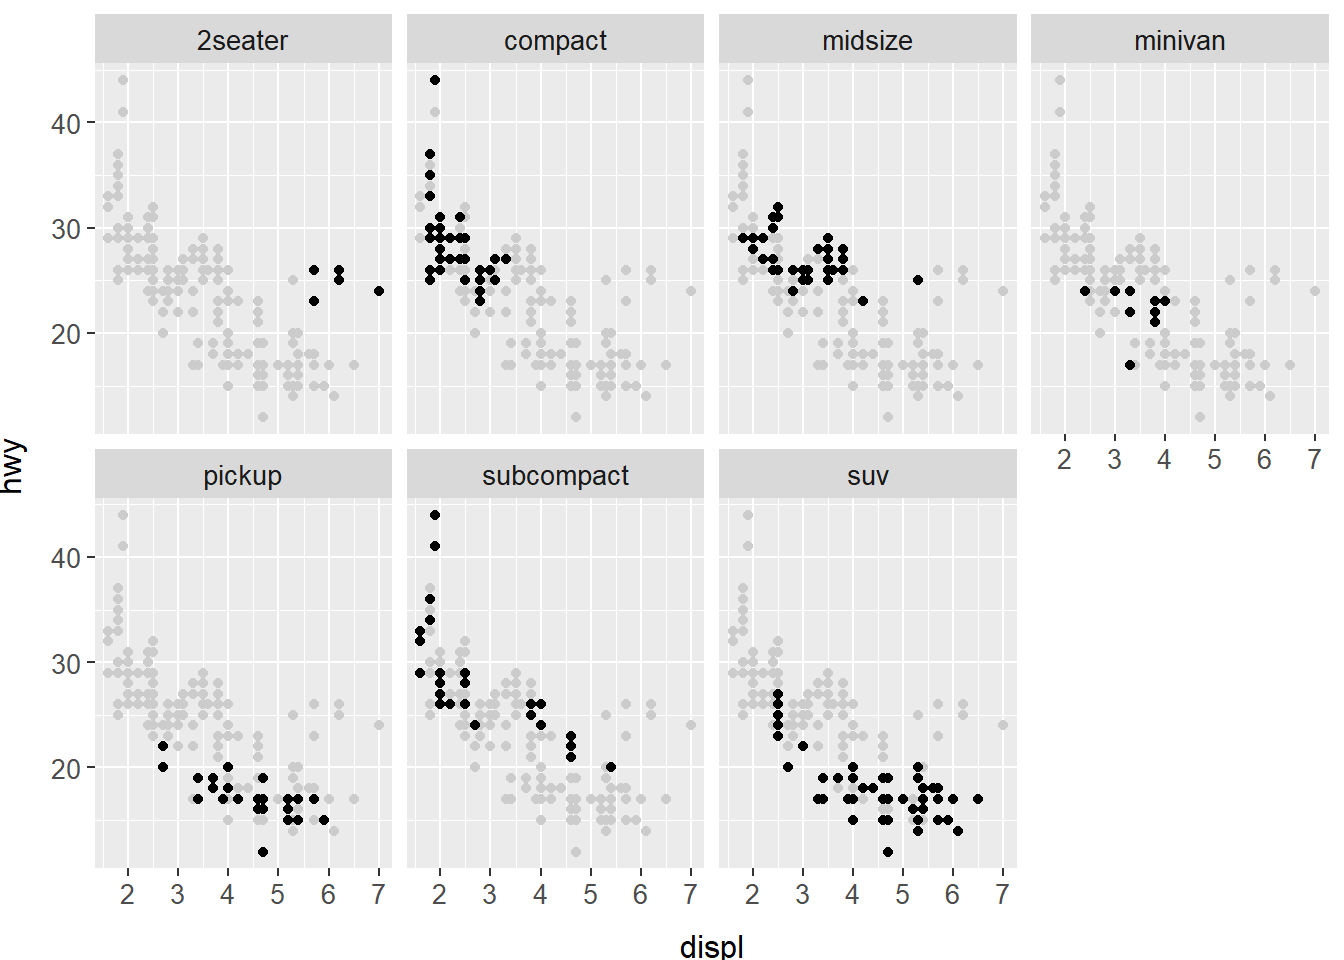
\includegraphics{r4ds_files/figure-latex/unnamed-chunk-21-1.pdf}

Quais são as vantagens de usar facetas, em vez de estética de cor? Quais são as desvantagens? Como o equilíbrio poderia mudar se você tivesse um conjunto de dados maior?

\begin{solution}
A principal vantagem no uso de facetas é que fica mais fácil analisar os dados quando eles estão separados em seu próprio contexto, contudo visualizá-los assim dificulta a comparação entre grupos.
\end{solution}

\hypertarget{exr1-5-5}{%
\subsection*{Exercício 1.5.5}\label{exr1-5-5}}
\addcontentsline{toc}{subsection}{Exercício 1.5.5}

Leia \texttt{?facet\_wrap}. O que \texttt{nrow} faz? o que \texttt{ncol} faz? Quais outras opções controlam o layout de paineis individuais? Por que \texttt{facet\_grid()} não tem variáveis \texttt{nrow}e \texttt{ncol}?

\begin{solution}
\leavevmode

\begin{verbatim}
?facet_wrap
\end{verbatim}

Os atributos \texttt{ncol} e \texttt{nrow} são utilizados pelo \texttt{facet\_wrap} para determinar o número de colunas ou linhas (respectivamente) nas quais serão distribuídos os gráficos segregados. Esses atributos não figuram em \texttt{facet\_grid} pelo fato deste já organizar as facetas retangularmente.

\end{solution}

\hypertarget{exr1-5-6}{%
\subsection*{Exercício 1.5.6}\label{exr1-5-6}}
\addcontentsline{toc}{subsection}{Exercício 1.5.6}

Ao usar \texttt{facet\_grid()} você normalmente deveria colocar a variável com níveis mais singulares nas colunas. Por quê?

\begin{solution}
Para melhor aproveitamento do espaço em tela.
\end{solution}

\hypertarget{objetos-geomuxe9tricos}{%
\section{Objetos geométricos}\label{objetos-geomuxe9tricos}}

\hypertarget{exr1-6-1}{%
\subsection*{Exercício 1.6.1}\label{exr1-6-1}}
\addcontentsline{toc}{subsection}{Exercício 1.6.1}

Que \emph{geom} você usaria para desenhar um gráfico de linha? Um diagrama de caixas (\emph{boxplot})? Um histograma? Um gráfico de área?

\begin{solution}
\leavevmode

\begin{Shaded}
\begin{Highlighting}[]
\FunctionTok{ggplot}\NormalTok{(}\AttributeTok{data =}\NormalTok{ mpg, }\AttributeTok{mapping =} \FunctionTok{aes}\NormalTok{(}\AttributeTok{x =}\NormalTok{ displ, }\AttributeTok{y =}\NormalTok{ hwy)) }\SpecialCharTok{+}
    \FunctionTok{geom\_line}\NormalTok{() }\SpecialCharTok{+}
\NormalTok{    tema}
\end{Highlighting}
\end{Shaded}

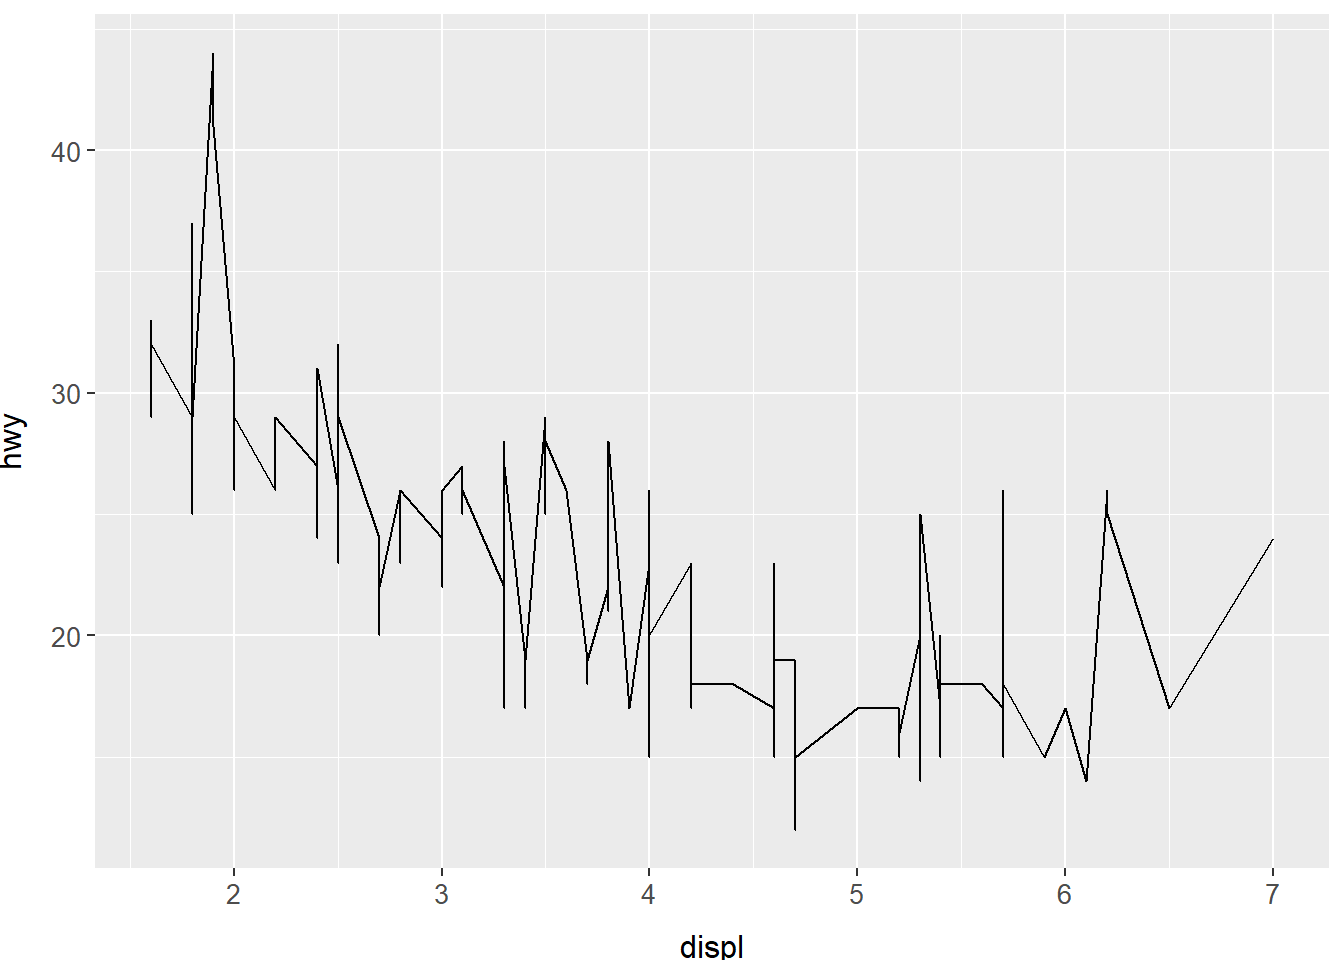
\includegraphics{r4ds_files/figure-latex/unnamed-chunk-22-1.pdf}

\begin{Shaded}
\begin{Highlighting}[]
\FunctionTok{ggplot}\NormalTok{(}\AttributeTok{data =}\NormalTok{ mpg) }\SpecialCharTok{+}
    \FunctionTok{geom\_boxplot}\NormalTok{(}\AttributeTok{mapping =} \FunctionTok{aes}\NormalTok{(}\AttributeTok{y =}\NormalTok{ hwy, }\AttributeTok{x =}\NormalTok{ class)) }\SpecialCharTok{+}
\NormalTok{    tema}
\end{Highlighting}
\end{Shaded}

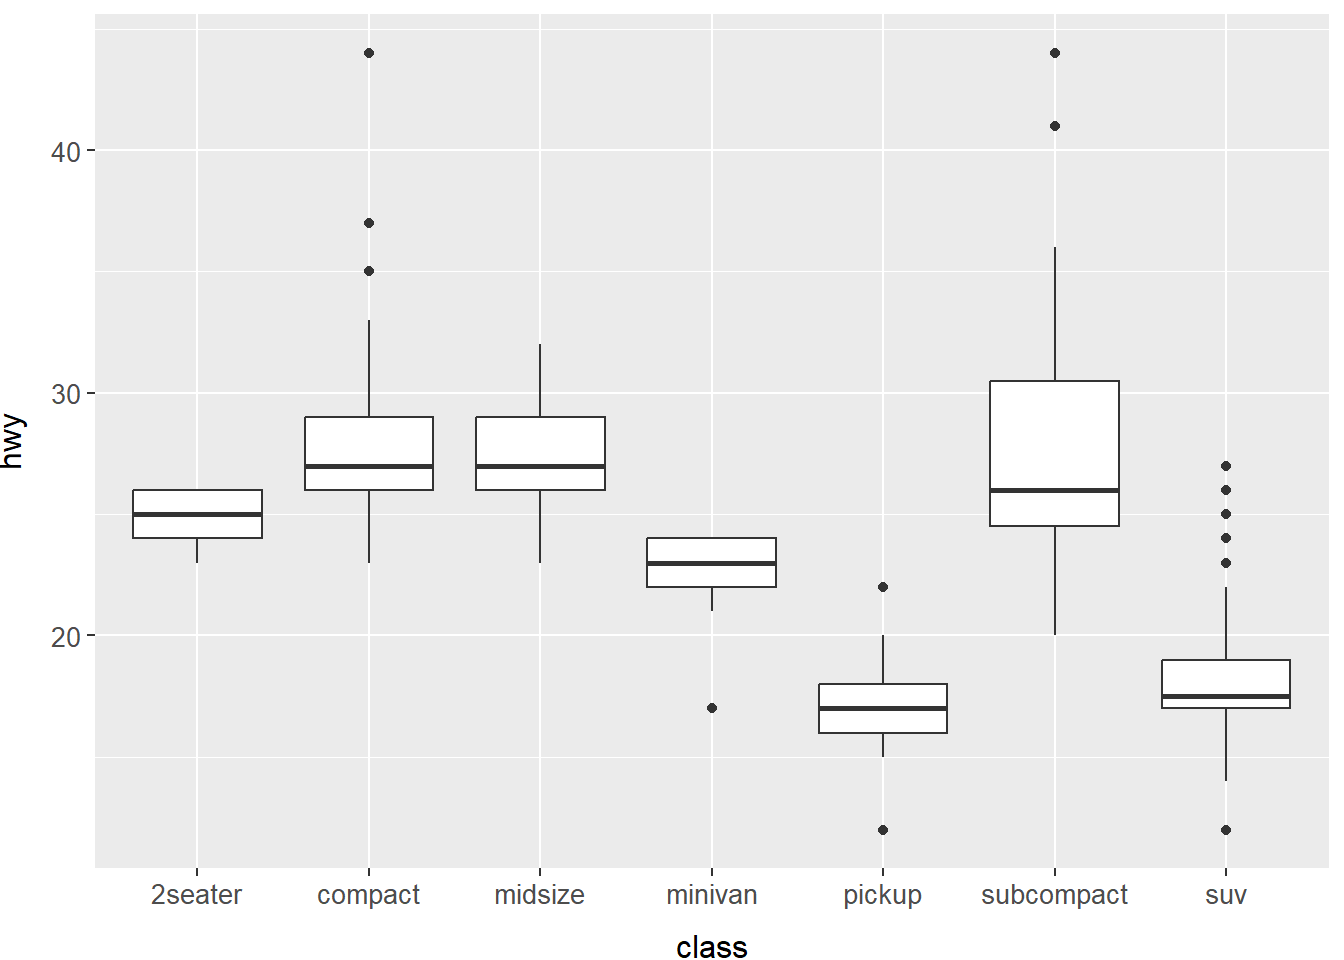
\includegraphics{r4ds_files/figure-latex/unnamed-chunk-23-1.pdf}

\begin{Shaded}
\begin{Highlighting}[]
\FunctionTok{ggplot}\NormalTok{(}\AttributeTok{data =}\NormalTok{ mpg, }\AttributeTok{mapping =} \FunctionTok{aes}\NormalTok{(}\AttributeTok{x =}\NormalTok{ hwy)) }\SpecialCharTok{+}
    \FunctionTok{geom\_histogram}\NormalTok{() }\SpecialCharTok{+}
\NormalTok{    tema}
\end{Highlighting}
\end{Shaded}

\begin{verbatim}
## `stat_bin()` using `bins = 30`. Pick better value with `binwidth`.
\end{verbatim}

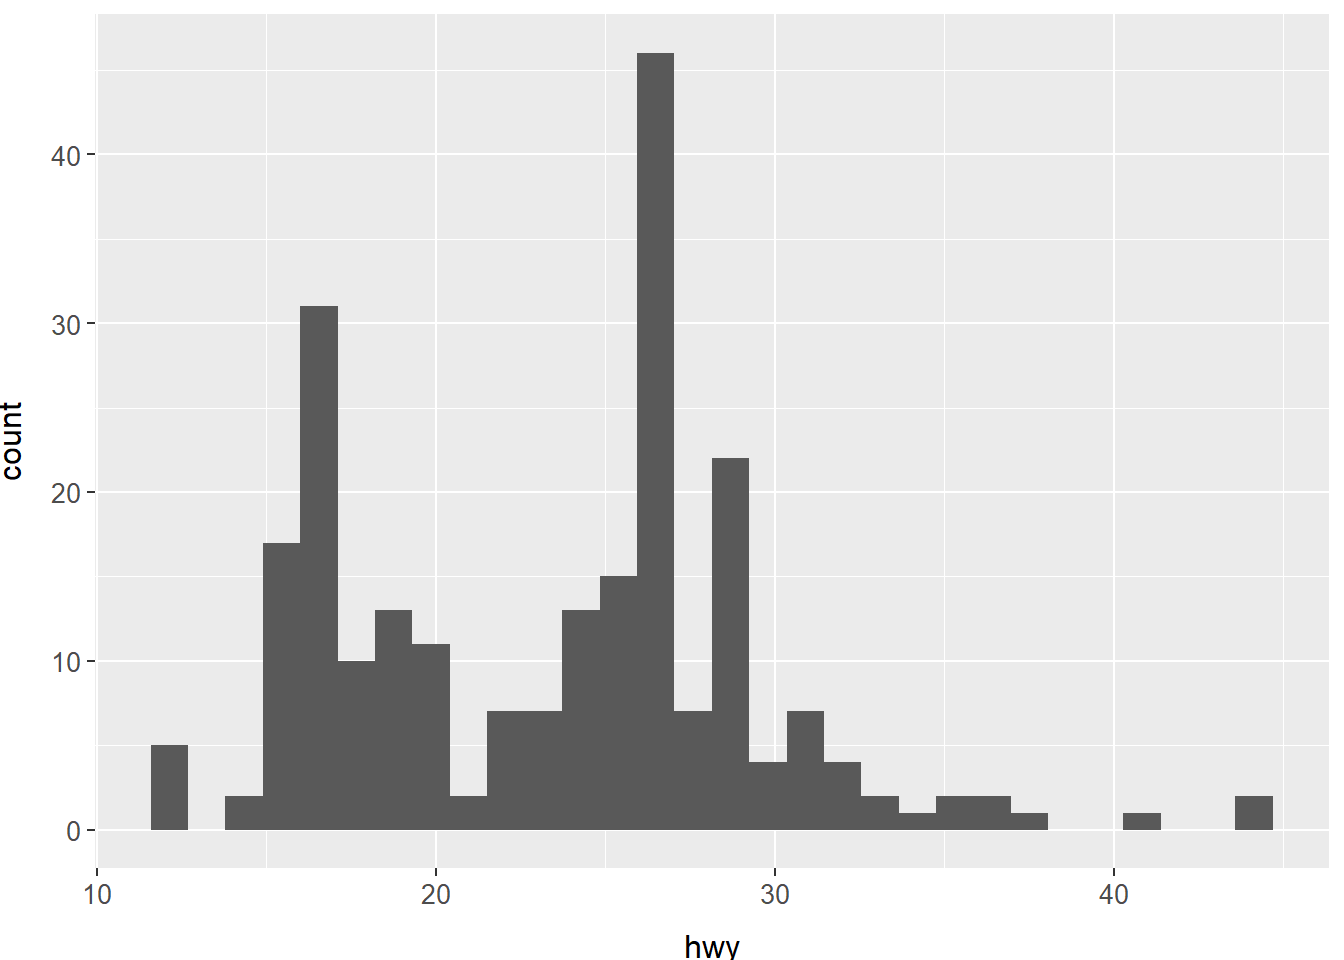
\includegraphics{r4ds_files/figure-latex/unnamed-chunk-24-1.pdf}

\begin{Shaded}
\begin{Highlighting}[]
\FunctionTok{ggplot}\NormalTok{(}\AttributeTok{data =}\NormalTok{ economics, }\AttributeTok{mapping =} \FunctionTok{aes}\NormalTok{(}\AttributeTok{x =}\NormalTok{ date, }\AttributeTok{y =}\NormalTok{ unemploy)) }\SpecialCharTok{+}
    \FunctionTok{geom\_area}\NormalTok{() }\SpecialCharTok{+}
\NormalTok{    tema}
\end{Highlighting}
\end{Shaded}

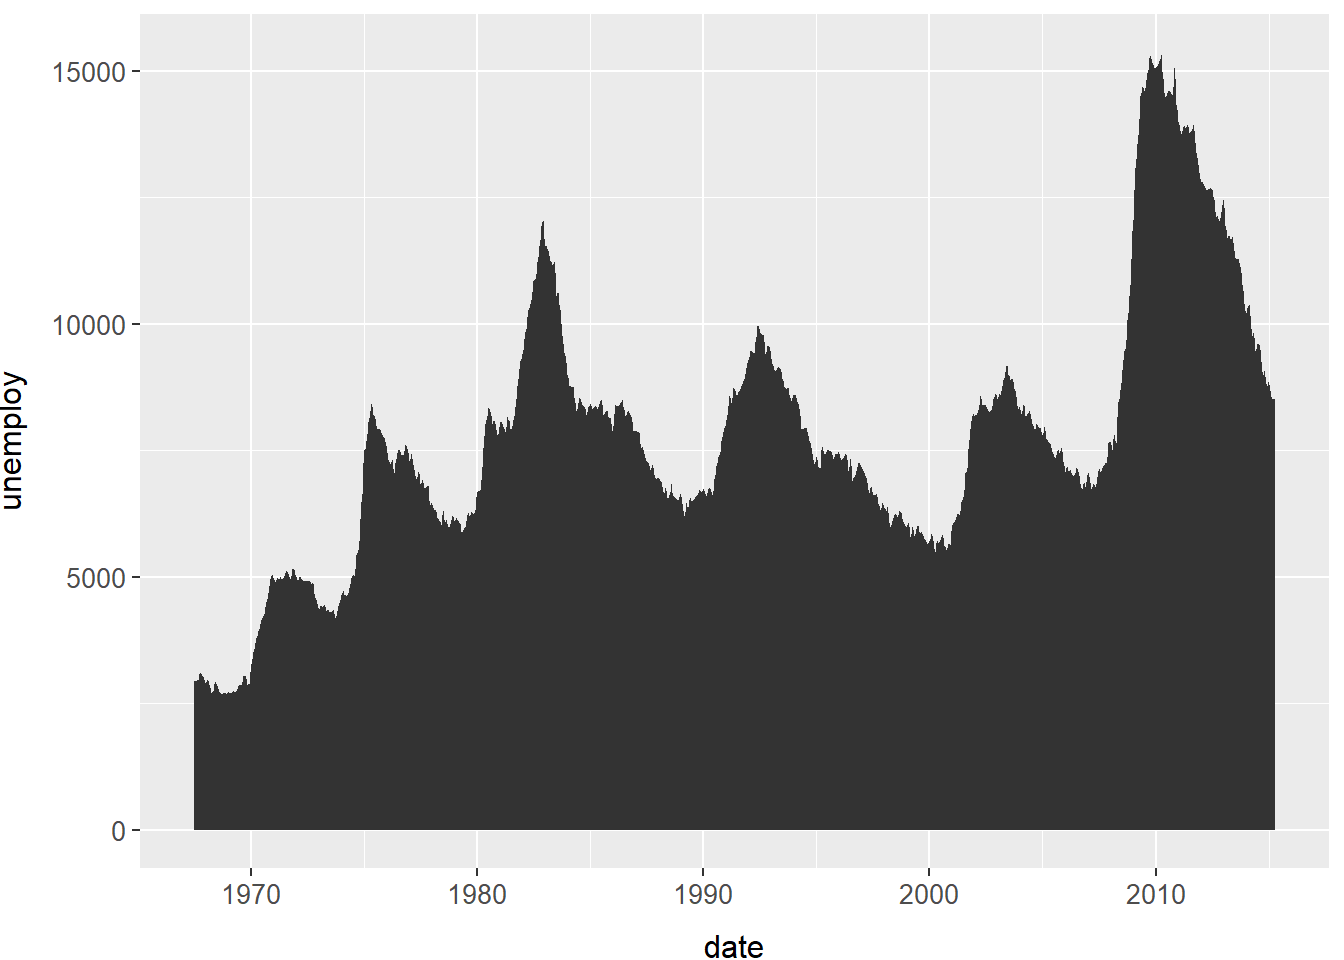
\includegraphics{r4ds_files/figure-latex/unnamed-chunk-25-1.pdf}

Podem ser utilizados, respectivamente as \emph{geoms}: \emph{line}, \emph{boxplot}, \emph{histogram} e \emph{area}.

\end{solution}

\hypertarget{exr1-6-2}{%
\subsection*{Exercício 1.6.2}\label{exr1-6-2}}
\addcontentsline{toc}{subsection}{Exercício 1.6.2}

Execute este código em sua cabeça e preveja como será o resultado. Depois execute o código no R e confira suas previsões:

\begin{Shaded}
\begin{Highlighting}[]
\FunctionTok{ggplot}\NormalTok{(}\AttributeTok{data =}\NormalTok{ mpg, }\AttributeTok{mapping =} \FunctionTok{aes}\NormalTok{(}\AttributeTok{x =}\NormalTok{ displ, }\AttributeTok{y =}\NormalTok{ hwy, }\AttributeTok{color =}\NormalTok{ drv)) }\SpecialCharTok{+}
    \FunctionTok{geom\_point}\NormalTok{() }\SpecialCharTok{+}
    \FunctionTok{geom\_smooth}\NormalTok{(}\AttributeTok{se =} \ConstantTok{FALSE}\NormalTok{) }\SpecialCharTok{+}
\NormalTok{    tema}
\end{Highlighting}
\end{Shaded}

\begin{verbatim}
## `geom_smooth()` using method = 'loess' and formula = 'y ~ x'
\end{verbatim}

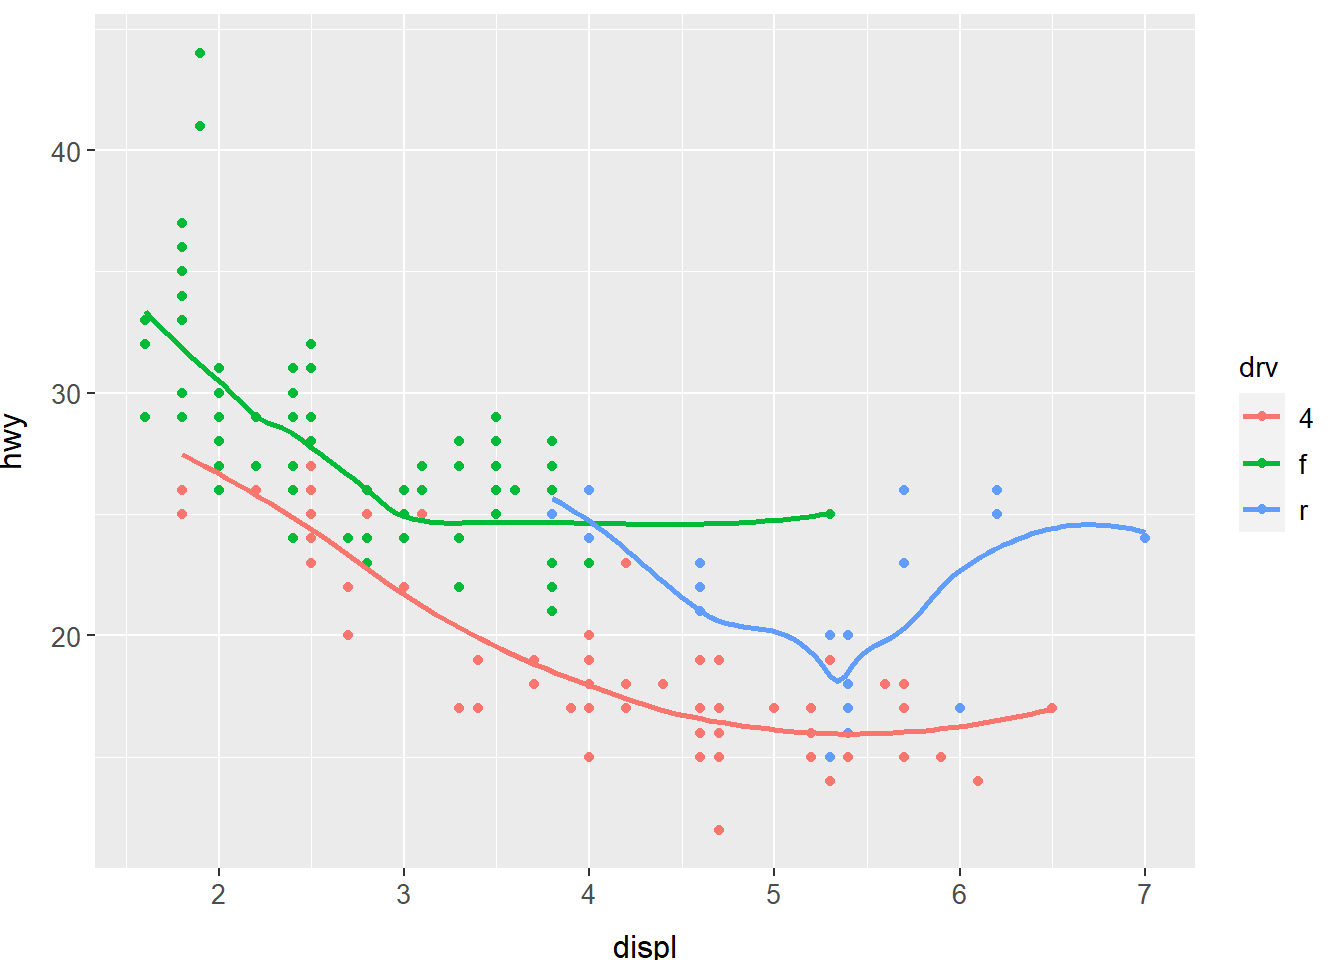
\includegraphics{r4ds_files/figure-latex/unnamed-chunk-26-1.pdf}

\begin{solution}
O gráfico bateu com a expectativa.
\end{solution}

\hypertarget{exr1-6-3}{%
\subsection*{Exercício 1.6.3}\label{exr1-6-3}}
\addcontentsline{toc}{subsection}{Exercício 1.6.3}

O que o \texttt{show.legend\ =\ FALSE} faz? O que acontece se você removê-lo? Por que você acha que usei isso anteriormente no capítulo?

\begin{solution}
\leavevmode

\begin{Shaded}
\begin{Highlighting}[]
\FunctionTok{ggplot}\NormalTok{(}\AttributeTok{data =}\NormalTok{ mpg, }\AttributeTok{mapping =} \FunctionTok{aes}\NormalTok{(}\AttributeTok{x =}\NormalTok{ displ, }\AttributeTok{y =}\NormalTok{ hwy, }\AttributeTok{color =}\NormalTok{ drv)) }\SpecialCharTok{+}
    \FunctionTok{geom\_point}\NormalTok{(}\AttributeTok{show.legend =} \ConstantTok{FALSE}\NormalTok{) }\SpecialCharTok{+}
    \FunctionTok{geom\_smooth}\NormalTok{(}\AttributeTok{se =} \ConstantTok{FALSE}\NormalTok{, }\AttributeTok{show.legend =} \ConstantTok{FALSE}\NormalTok{) }\SpecialCharTok{+}
\NormalTok{    tema}
\end{Highlighting}
\end{Shaded}

\begin{verbatim}
## `geom_smooth()` using method = 'loess' and formula = 'y ~ x'
\end{verbatim}

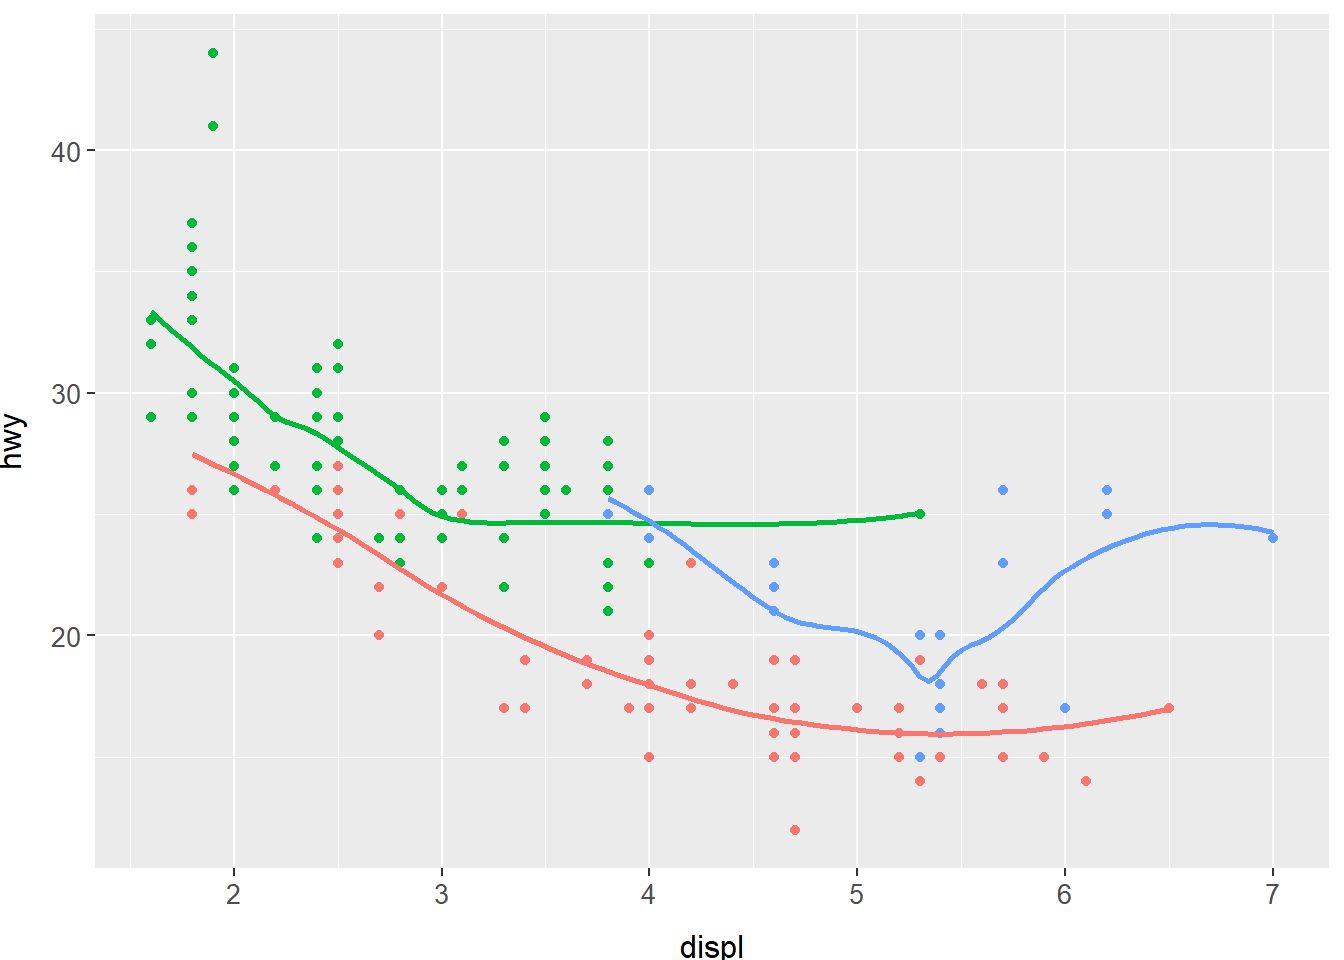
\includegraphics{r4ds_files/figure-latex/unnamed-chunk-27-1.pdf}

Ele indica que, para a camada à qual se aplica, não serão geradas as legendas de identificação.

\end{solution}

\hypertarget{exr1-6-4}{%
\subsection*{Exercício 1.6.4}\label{exr1-6-4}}
\addcontentsline{toc}{subsection}{Exercício 1.6.4}

O que o argumento \texttt{se} para \texttt{geom\_smooth} faz?

\begin{solution}
\leavevmode

\begin{verbatim}
?geom_smooth
\end{verbatim}

Esse argumento indica se o intervalo de confiança utilizado no processo de suavização da linha deve ou não ser exibido no gráfico.

\end{solution}

\hypertarget{exr1-6-5}{%
\subsection*{Exercício 1.6.5}\label{exr1-6-5}}
\addcontentsline{toc}{subsection}{Exercício 1.6.5}

Esses dois gráficos serão diferentes? Por quê/por que não?

\begin{verbatim}
ggplot(data = mpg, mapping = aes(x = displ, y = hwy)) +
    geom_point() +
    geom_smooth() +
    tema
    
ggplot() + 
    geom_point(data = mpg, mapping = aes(x = displ, y = hwy)) +
    geom_smooth(data = mpg, mapping = aes(x = displ, y = hwy)) +
    tema
\end{verbatim}

\begin{solution}
Os gráficos serão iguais. Ao informar os parâmetros \texttt{data} e \texttt{mapping} na função \texttt{ggplot} essas atributos serão considerados como globais, sendo utilizado em todos as camadas do gráfico, a menos que alguma das camadas os sobrescreva. No segundo gráfico, não são definidos parâmetros globais, porém, o mesmo parâmetro é passado para ambas as camadas, sendo assim, a única diferença é o código estar duplicado.
\end{solution}

\hypertarget{exr1-6-6}{%
\subsection*{Exercício 1.6.6}\label{exr1-6-6}}
\addcontentsline{toc}{subsection}{Exercício 1.6.6}

Recrie o código R necessário para gerar os seguintes gráficos:

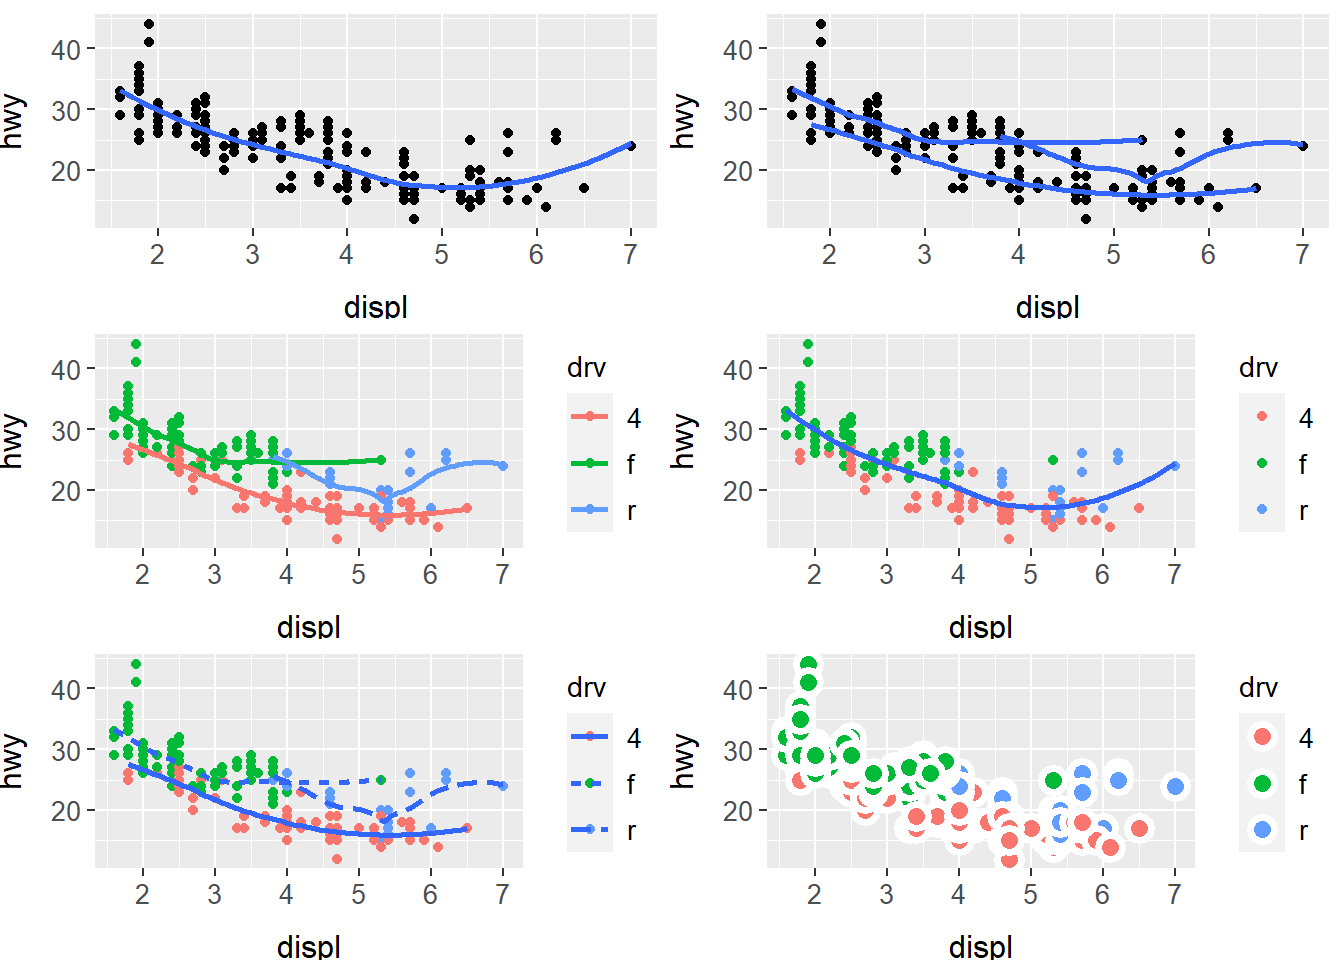
\includegraphics{r4ds_files/figure-latex/unnamed-chunk-28-1.pdf}

\begin{solution}
\leavevmode

\begin{verbatim}
a <- ggplot(data = mpg, mapping = aes(x = displ, y = hwy)) +
        geom_point() +
        geom_smooth(se = FALSE) +
        tema

b <- ggplot(data = mpg, mapping = aes(x = displ, y = hwy)) +
        geom_point() +
        geom_smooth(mapping = aes(group = drv), se = FALSE) +
        tema

c <- ggplot(data = mpg, mapping = aes(x = displ, y = hwy, color = drv)) +
        geom_point() +
        geom_smooth(se = FALSE) +
        tema

d <- ggplot(data = mpg, mapping = aes(x = displ, y = hwy)) +
        geom_point(mapping = aes(color = drv)) +
        geom_smooth(se = FALSE) +
        tema

e <- ggplot(data = mpg, mapping = aes(x = displ, y = hwy)) +
        geom_point(mapping = aes(color = drv)) +
        geom_smooth(mapping = aes(linetype = drv), se = FALSE) +
        tema

f <- ggplot(data = mpg, mapping = aes(x = displ, y = hwy, fill = drv)) +
        geom_point(color = "white", shape = 21, size = 3, stroke = 2) +
        tema
\end{verbatim}

\end{solution}

\hypertarget{transformauxe7uxf5es-estatuxedsticas}{%
\section{Transformações estatísticas}\label{transformauxe7uxf5es-estatuxedsticas}}

\hypertarget{exr1-7-1}{%
\subsection*{Exercício 1.7.1}\label{exr1-7-1}}
\addcontentsline{toc}{subsection}{Exercício 1.7.1}

Qual é o \texttt{geom} padrão associado ao \texttt{stat\_summary()}? Como você poderia reescrever o gráfico anterior usando essa função \texttt{geom}, em vez da função \texttt{stat}?

\begin{solution}
\leavevmode

\begin{verbatim}
?stat_summary
\end{verbatim}

\begin{Shaded}
\begin{Highlighting}[]
\FunctionTok{ggplot}\NormalTok{(}\AttributeTok{data =}\NormalTok{ diamonds) }\SpecialCharTok{+}
    \FunctionTok{stat\_summary}\NormalTok{(}
        \AttributeTok{mapping =} \FunctionTok{aes}\NormalTok{(}\AttributeTok{x =}\NormalTok{ cut, }\AttributeTok{y =}\NormalTok{ depth),}
        \AttributeTok{fun.min =}\NormalTok{ min,}
        \AttributeTok{fun.max =}\NormalTok{ max,}
        \AttributeTok{fun =}\NormalTok{ median}
\NormalTok{    ) }\SpecialCharTok{+}
\NormalTok{    tema}
\end{Highlighting}
\end{Shaded}

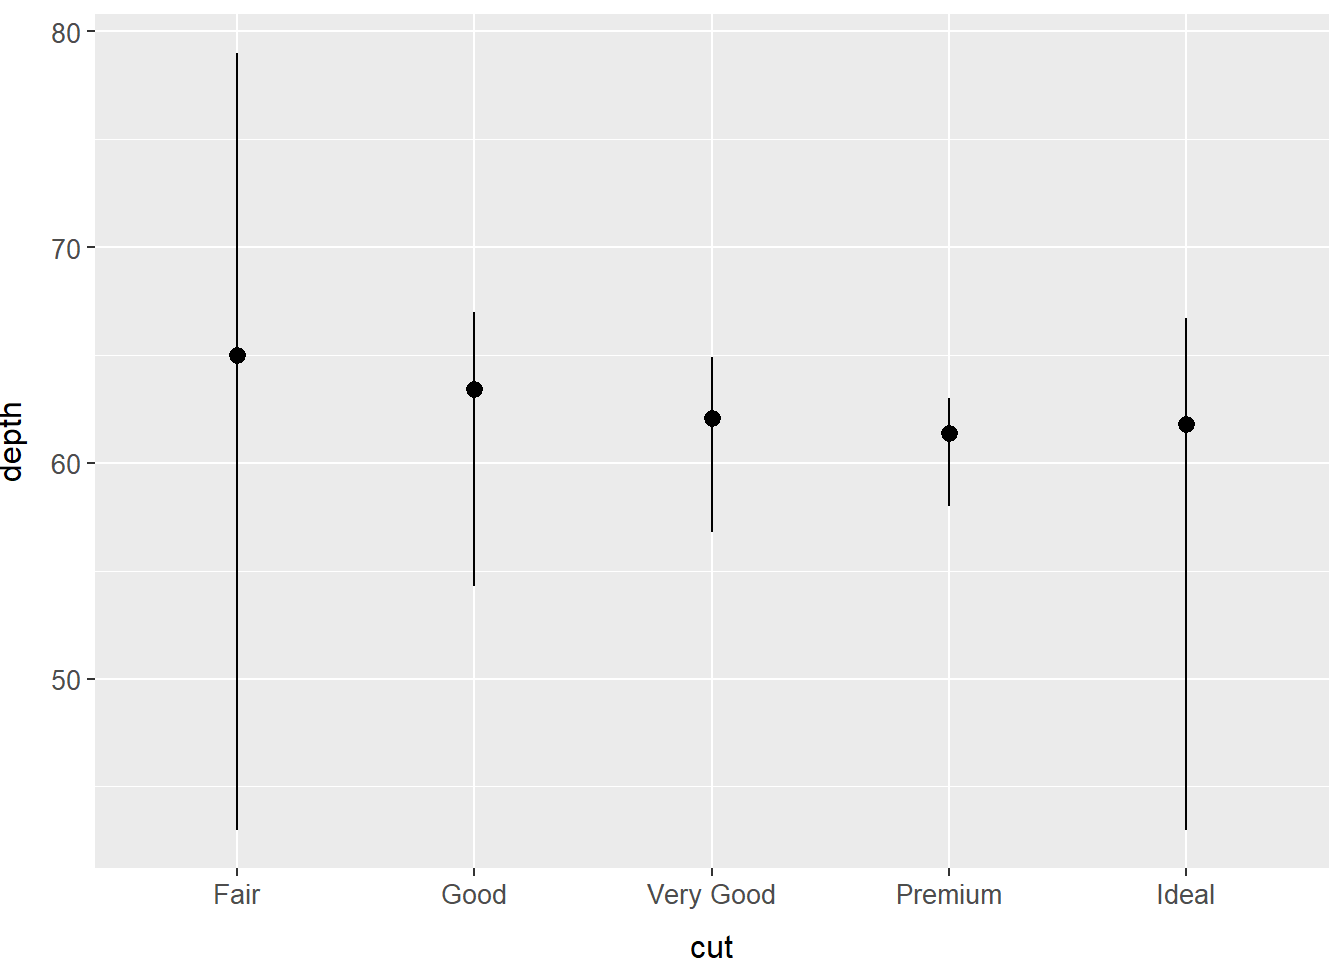
\includegraphics{r4ds_files/figure-latex/unnamed-chunk-29-1.pdf}

A \texttt{geom} associada é a \texttt{geom\_pointrange} e o gráfico poderia ser reescrito da seguinte maneira.

\end{solution}

\hypertarget{exr1-7-2}{%
\subsection*{Exercício 1.7.2}\label{exr1-7-2}}
\addcontentsline{toc}{subsection}{Exercício 1.7.2}

O que \texttt{geom\_col()} faz? Qual é a diferença entre ele e \texttt{geom\_bar()}?

\begin{solution}
\leavevmode

\begin{Shaded}
\begin{Highlighting}[]
\FunctionTok{ggplot}\NormalTok{(}\AttributeTok{data =}\NormalTok{ diamonds, }\AttributeTok{mapping =} \FunctionTok{aes}\NormalTok{(}\AttributeTok{x =}\NormalTok{ cut)) }\SpecialCharTok{+}
    \FunctionTok{geom\_bar}\NormalTok{() }\SpecialCharTok{+}
\NormalTok{    tema}
\end{Highlighting}
\end{Shaded}

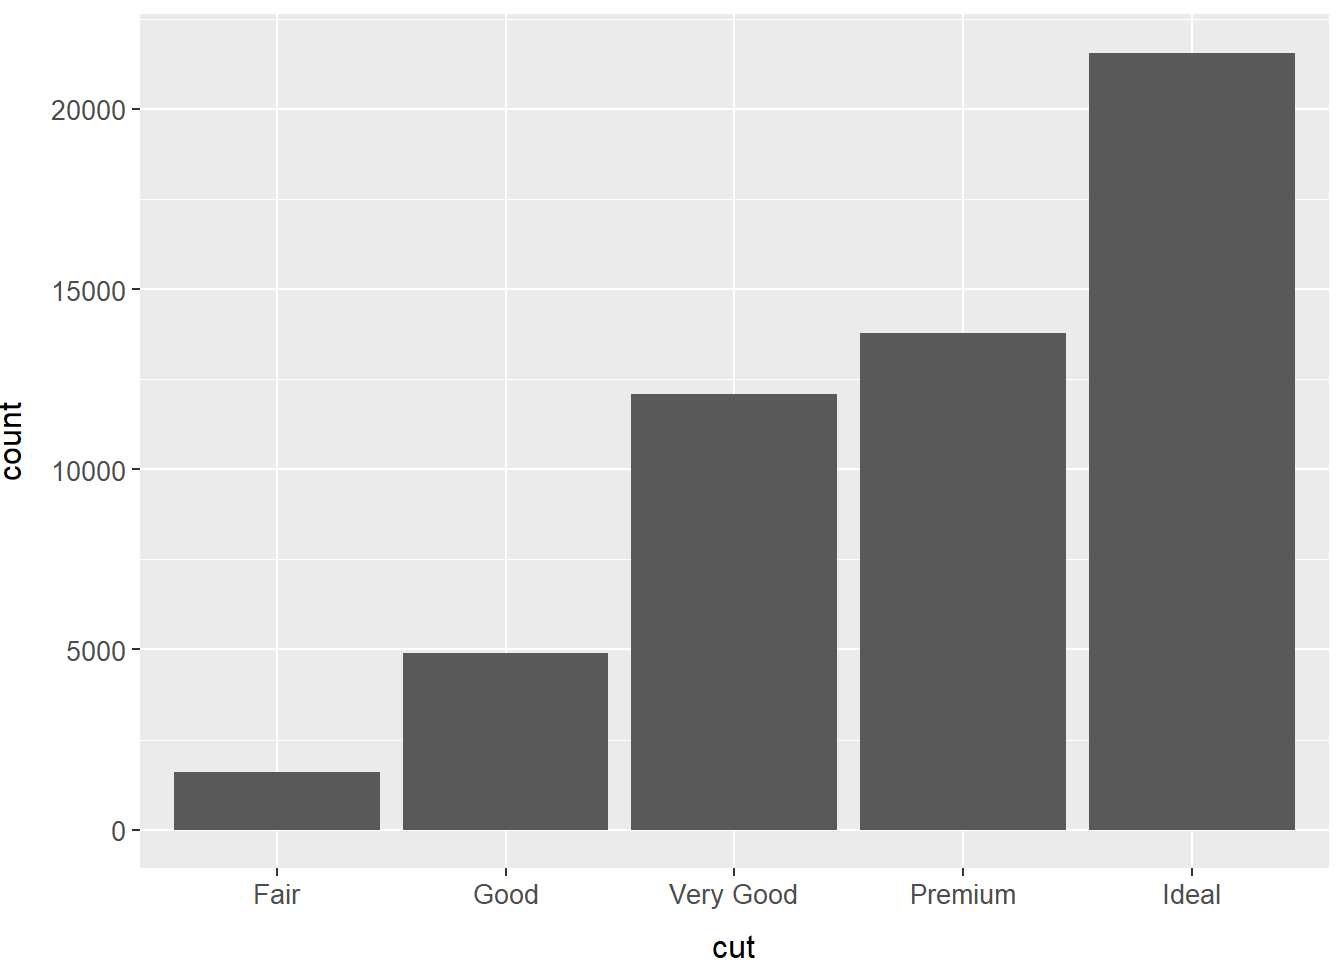
\includegraphics{r4ds_files/figure-latex/unnamed-chunk-30-1.pdf}

\begin{Shaded}
\begin{Highlighting}[]
\FunctionTok{ggplot}\NormalTok{(}\AttributeTok{data =}\NormalTok{ diamonds, }\AttributeTok{mapping =} \FunctionTok{aes}\NormalTok{(}\AttributeTok{x =}\NormalTok{ cut, }\AttributeTok{y =}\NormalTok{ carat)) }\SpecialCharTok{+}
    \FunctionTok{geom\_col}\NormalTok{() }\SpecialCharTok{+}
\NormalTok{    tema}
\end{Highlighting}
\end{Shaded}

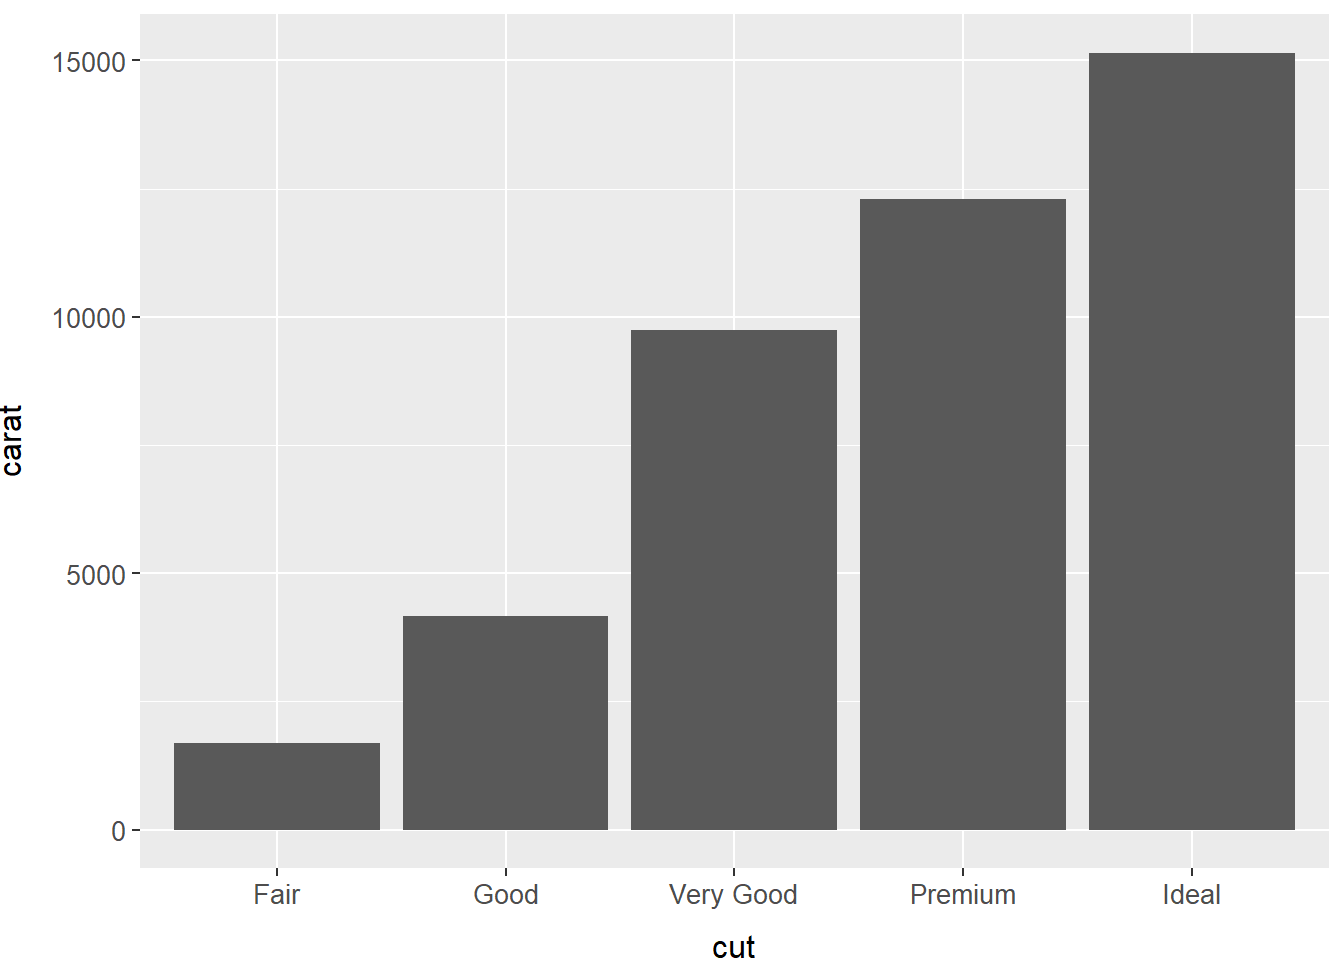
\includegraphics{r4ds_files/figure-latex/unnamed-chunk-31-1.pdf}

Enquanto no \texttt{geom\_bar} a altura das barras representa uma transformação estatística relacionada às observações (como \texttt{count}, por exemplo), no \texttt{geom\_col} podemos exibir o acumulado (soma) de uma variável para cada categoria exibida.

\end{solution}

\hypertarget{exr1-7-3}{%
\subsection*{Exercício 1.7.3}\label{exr1-7-3}}
\addcontentsline{toc}{subsection}{Exercício 1.7.3}

A maioria dos \texttt{geoms} e \texttt{stats} vem em pares, que são quase sempre usados juntos. Leia a documentação e faça uma lista de todos os pares. O que eles têm em comum?

\begin{solution}
\leavevmode

\begin{longtable}[]{@{}ccc@{}}
\toprule\noalign{}
\# & Geom & Stat \\
\midrule\noalign{}
\endhead
\bottomrule\noalign{}
\endlastfoot
01 & Blank & Identity \\
02 & Curve & Identity \\
03 & Segment & Identity \\
04 & Path & Identity \\
05 & Line & Identity \\
06 & Step & Identity \\
07 & Poligon & Identity \\
08 & Raster & Identity \\
09 & Rect & Identity \\
10 & Tile & Identity \\
11 & Ribbon & Identity \\
12 & Area & Identity \\
13 & Align & ? \\
14 & ABLine & ? \\
15 & HLine & ? \\
16 & Density & Density \\
17 & DotPlot & ? \\
18 & Freqpoly & Bin \\
19 & Histogram & Bin \\
20 & Col & Identity \\
21 & Bar & Count \\
22 & Label & Identity \\
23 & Text & Identity \\
24 & Jitter & Identity \\
25 & Point & Identity \\
26 & Quantile & Quantile \\
27 & Rug & Identity \\
28 & Boxplot & Boxplot \\
29 & Violin & YDensity \\
30 & Count & Sum \\
31 & Bin 2D & Bin 2D \\
32 & Density 2D & Density 2D \\
33 & Hex & Bin Hex \\
34 & Cross Bar & Identity \\
35 & Error Bar & Identity \\
36 & Line Range & Identity \\
37 & Point Range & Identity \\
38 & Map & Identity \\
39 & Contour & Contour \\
40 & Contour Filled & Contour Filled \\
\end{longtable}

\end{solution}

\hypertarget{exr1-7-4}{%
\subsection*{Exercício 1.7.4}\label{exr1-7-4}}
\addcontentsline{toc}{subsection}{Exercício 1.7.4}

Quais variáveis \texttt{stat\_smooth()} calcula? Quais parâmetros controlam seu comportamento?

\begin{solution}
\leavevmode

\begin{verbatim}
?stat_smooth
\end{verbatim}

\end{solution}

\hypertarget{exr1-7-5}{%
\subsection*{Exercício 1.7.5}\label{exr1-7-5}}
\addcontentsline{toc}{subsection}{Exercício 1.7.5}

Em nosso gráfico de barra de \emph{proportion}, precisamos configurar \texttt{group\ =\ 1}. Por quê? Em outras palavras, qual é o problema com esses dois gráficos?

\begin{Shaded}
\begin{Highlighting}[]
\FunctionTok{ggplot}\NormalTok{(}\AttributeTok{data =}\NormalTok{ diamonds) }\SpecialCharTok{+}
    \FunctionTok{geom\_bar}\NormalTok{(}\AttributeTok{mapping =} \FunctionTok{aes}\NormalTok{(}\AttributeTok{x =}\NormalTok{ cut, }\AttributeTok{y =} \FunctionTok{after\_stat}\NormalTok{(prop), }\AttributeTok{group =} \DecValTok{1}\NormalTok{)) }\SpecialCharTok{+}
\NormalTok{    tema}
\end{Highlighting}
\end{Shaded}

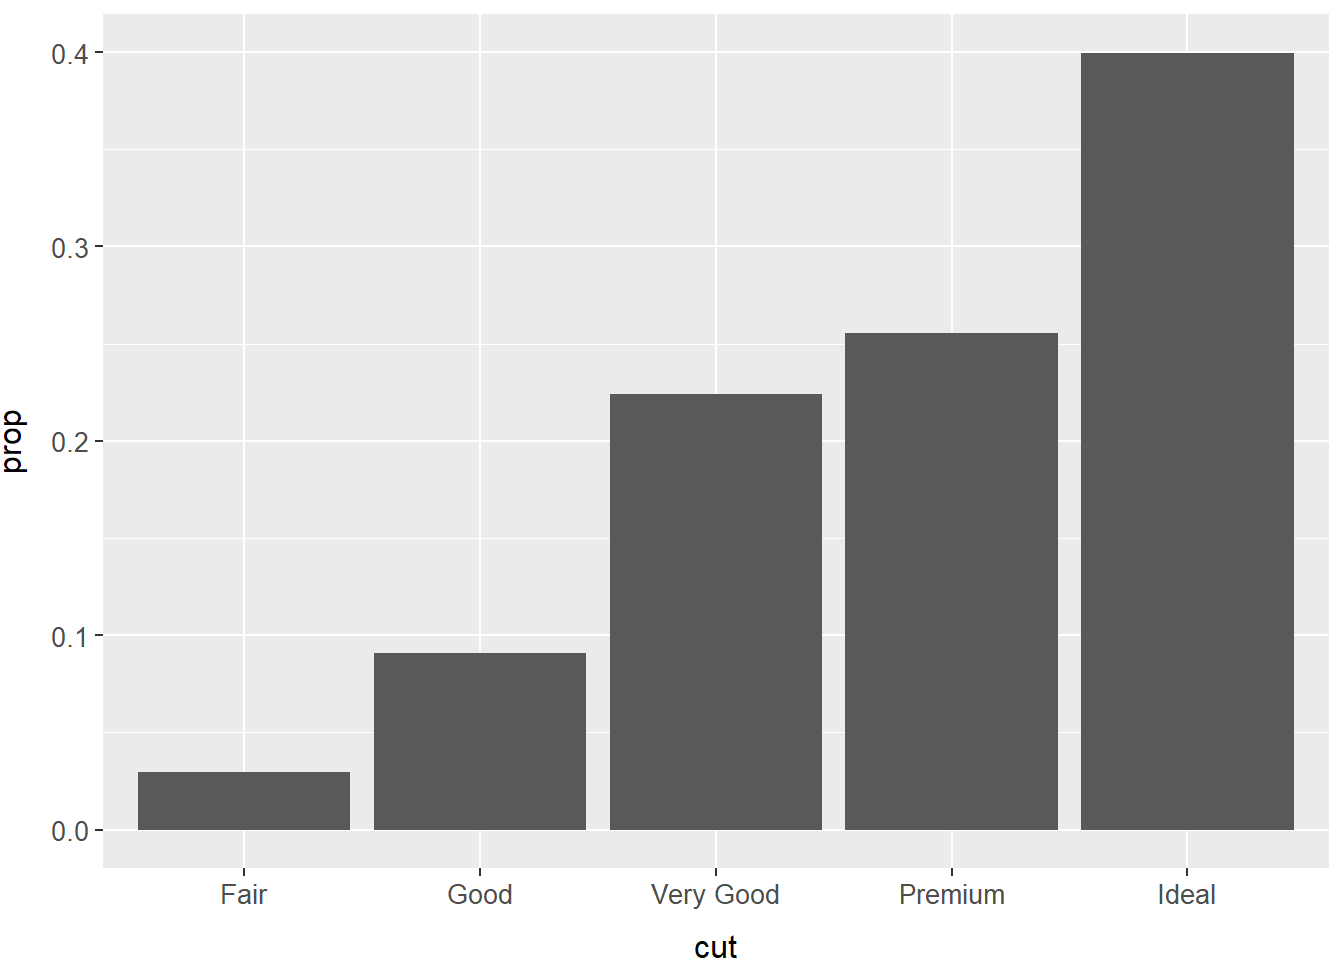
\includegraphics{r4ds_files/figure-latex/unnamed-chunk-32-1.pdf}

\begin{solution}
\leavevmode

\begin{Shaded}
\begin{Highlighting}[]
\FunctionTok{ggplot}\NormalTok{(}\AttributeTok{data =}\NormalTok{ diamonds) }\SpecialCharTok{+}
    \FunctionTok{geom\_bar}\NormalTok{(}\AttributeTok{mapping =} \FunctionTok{aes}\NormalTok{(}
        \AttributeTok{x =}\NormalTok{ cut, }
        \AttributeTok{fill =}\NormalTok{ color, }
        \AttributeTok{y =} \FunctionTok{after\_stat}\NormalTok{(prop), }
        \AttributeTok{group =}\NormalTok{ color}
\NormalTok{    )) }\SpecialCharTok{+}
\NormalTok{    tema}
\end{Highlighting}
\end{Shaded}

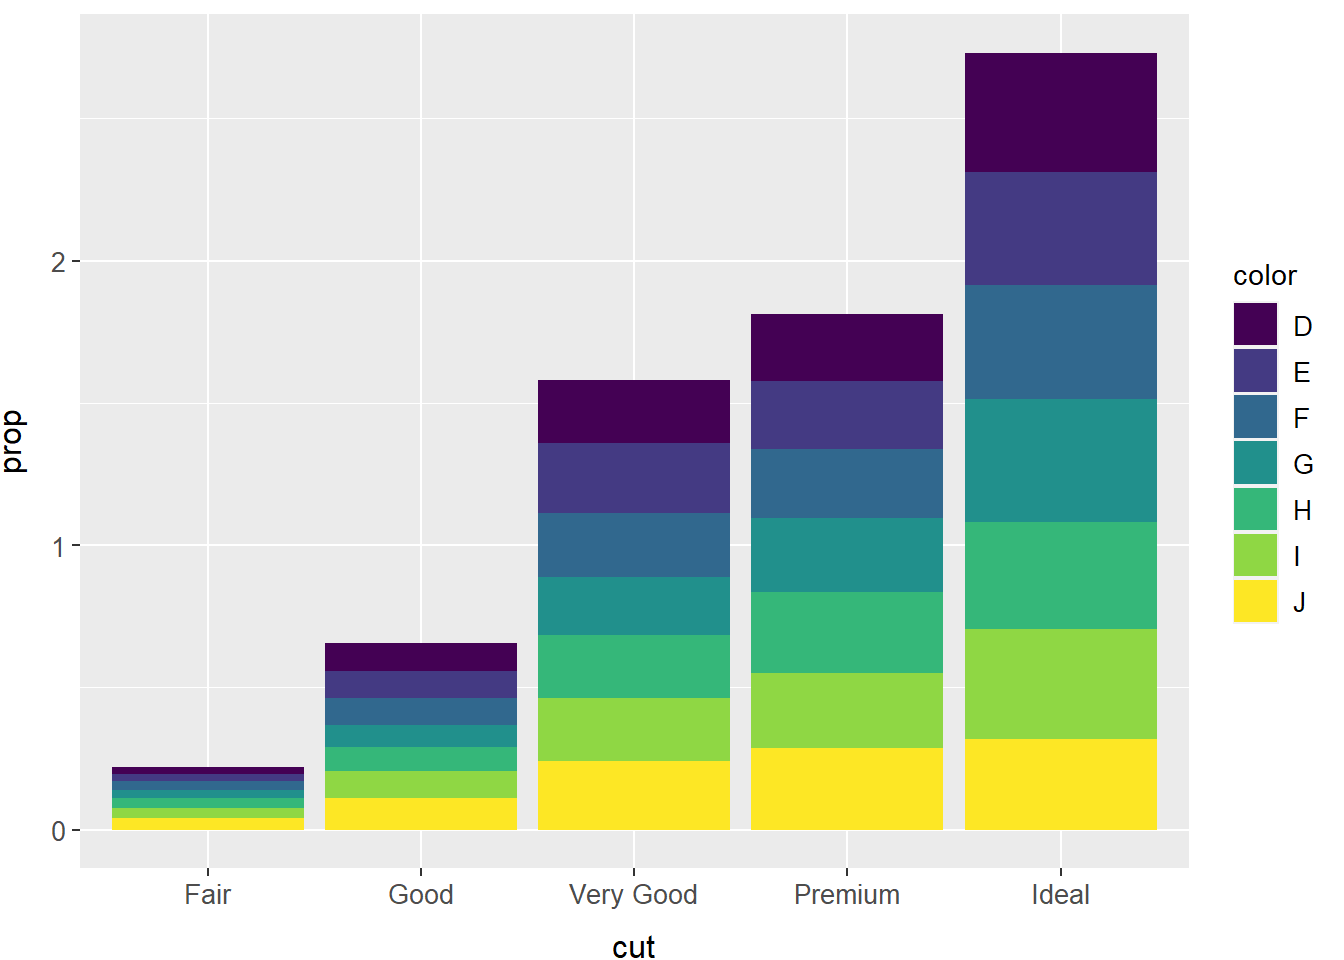
\includegraphics{r4ds_files/figure-latex/unnamed-chunk-33-1.pdf}

Quando estamos trabalhando com proporções (ou estátisticas em geral), é importante destacar para o \texttt{ggplot} qual agrupamento ele deve considerar, caso contrário ele irá considerar um único grupo e dará uma impressão incorreta ao gráfico. No primeiro exemplo, foi utilizado \texttt{group\ =\ 1} (e, na verdade, poderia ser qualquer valor) apenas para indicar que deveria ser realizado um agrupamento.

\end{solution}

\hypertarget{ajustes-de-posiuxe7uxe3o}{%
\section{Ajustes de posição}\label{ajustes-de-posiuxe7uxe3o}}

\hypertarget{exr1-8-1}{%
\subsection*{Exercício 1.8.1}\label{exr1-8-1}}
\addcontentsline{toc}{subsection}{Exercício 1.8.1}

Qual é o problema com este gráfico? Como você poderia melhorá-lo?

\begin{Shaded}
\begin{Highlighting}[]
\FunctionTok{ggplot}\NormalTok{(}\AttributeTok{data =}\NormalTok{ mpg, }\AttributeTok{mapping =} \FunctionTok{aes}\NormalTok{(}\AttributeTok{x =}\NormalTok{ cty, }\AttributeTok{y =}\NormalTok{ hwy)) }\SpecialCharTok{+}
    \FunctionTok{geom\_point}\NormalTok{() }\SpecialCharTok{+}
\NormalTok{    tema}
\end{Highlighting}
\end{Shaded}

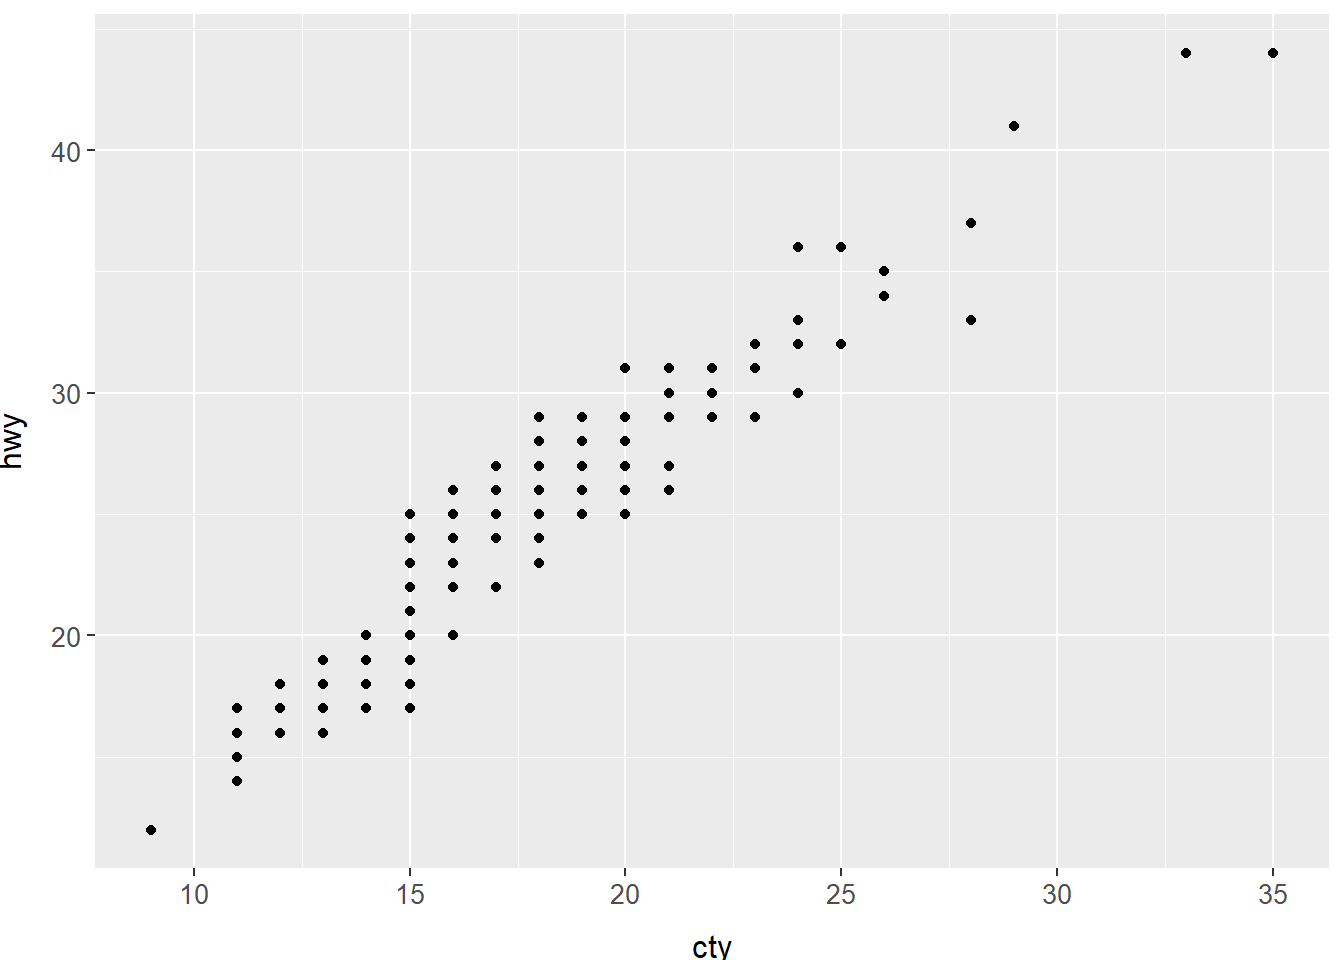
\includegraphics{r4ds_files/figure-latex/unnamed-chunk-34-1.pdf}

\begin{solution}
Há pontos sobrepostos. Uma melhoria poderia ser usar \texttt{geom\_jitter} em lugar de \texttt{geom\_point}.

\begin{Shaded}
\begin{Highlighting}[]
\FunctionTok{ggplot}\NormalTok{(}\AttributeTok{data =}\NormalTok{ mpg, }\AttributeTok{mapping =} \FunctionTok{aes}\NormalTok{(}\AttributeTok{x =}\NormalTok{ cty, }\AttributeTok{y =}\NormalTok{ hwy)) }\SpecialCharTok{+}
    \FunctionTok{geom\_jitter}\NormalTok{() }\SpecialCharTok{+}
\NormalTok{    tema}
\end{Highlighting}
\end{Shaded}

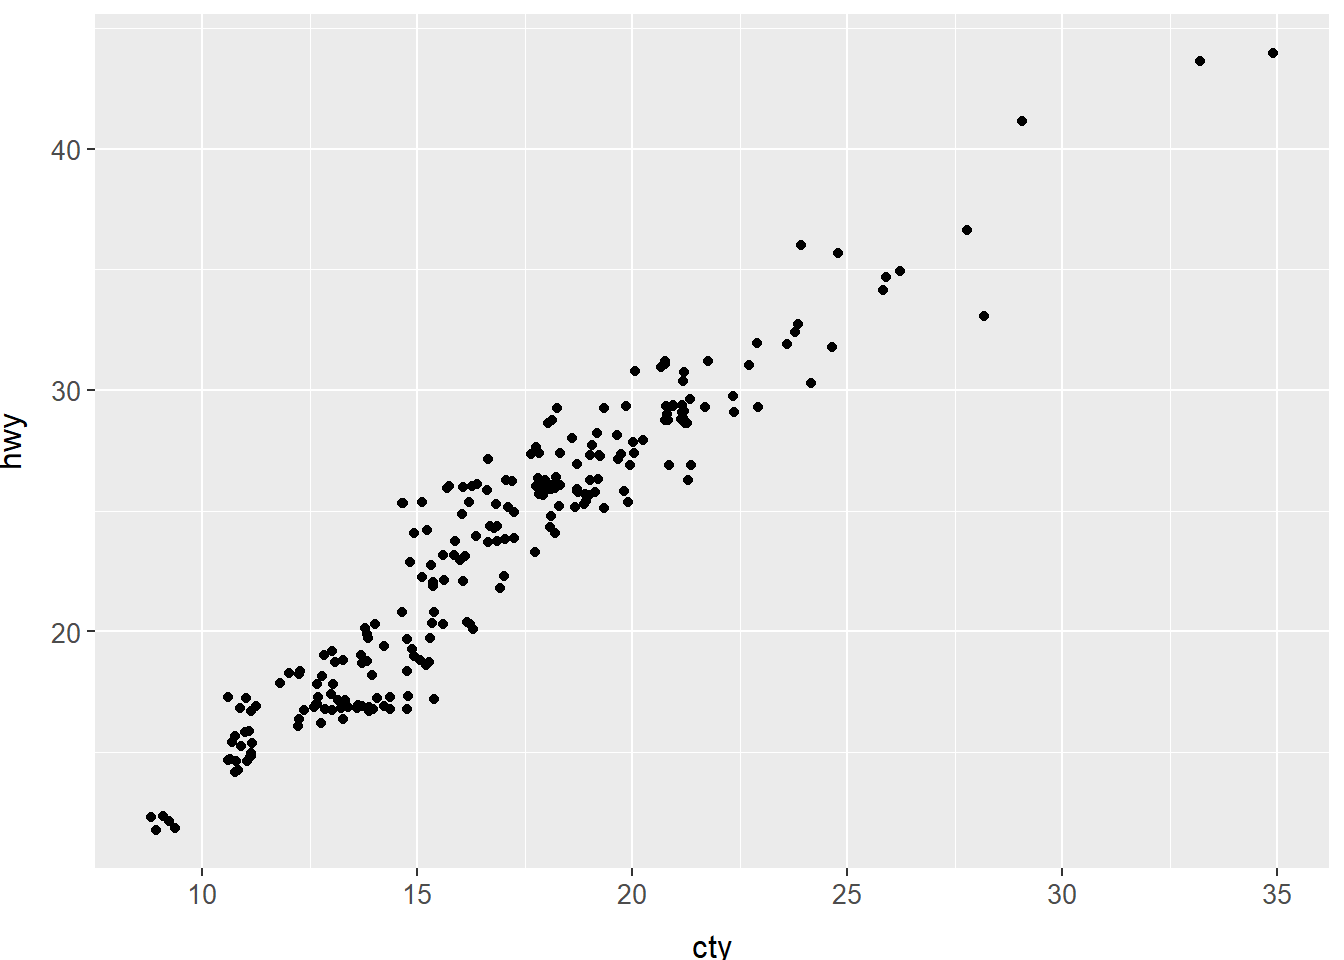
\includegraphics{r4ds_files/figure-latex/unnamed-chunk-35-1.pdf}
\end{solution}

\hypertarget{exr1-8-2}{%
\subsection*{Exercício 1.8.2}\label{exr1-8-2}}
\addcontentsline{toc}{subsection}{Exercício 1.8.2}

Quais parâmetros para \texttt{geom\_jitter} controlam a quantidade de oscilação?

\begin{solution}
Conforme a documentação disposta em \texttt{?geom\_jitter}, são utilizados os parâmetros \texttt{width} e \texttt{height}.
\end{solution}

\hypertarget{exr1-8-3}{%
\subsection*{Exercício 1.8.3}\label{exr1-8-3}}
\addcontentsline{toc}{subsection}{Exercício 1.8.3}

Compare o contraste entre \texttt{geom\_jitter} e \texttt{geom\_count}.

\begin{solution}
\leavevmode

\begin{Shaded}
\begin{Highlighting}[]
\NormalTok{a }\OtherTok{\textless{}{-}} \FunctionTok{ggplot}\NormalTok{(}\AttributeTok{data =}\NormalTok{ mpg, }\AttributeTok{mapping =} \FunctionTok{aes}\NormalTok{(}\AttributeTok{x =}\NormalTok{ cty, }\AttributeTok{y =}\NormalTok{ hwy)) }\SpecialCharTok{+}
      \FunctionTok{geom\_jitter}\NormalTok{() }\SpecialCharTok{+}
\NormalTok{      tema}

\NormalTok{b }\OtherTok{\textless{}{-}} \FunctionTok{ggplot}\NormalTok{(}\AttributeTok{data =}\NormalTok{ mpg, }\AttributeTok{mapping =} \FunctionTok{aes}\NormalTok{(}\AttributeTok{x =}\NormalTok{ cty, }\AttributeTok{y =}\NormalTok{ hwy)) }\SpecialCharTok{+}
      \FunctionTok{geom\_count}\NormalTok{(}\AttributeTok{show.legend =} \ConstantTok{FALSE}\NormalTok{) }\SpecialCharTok{+}
\NormalTok{      tema}

\FunctionTok{grid.arrange}\NormalTok{(a, b, }\AttributeTok{nrow =} \DecValTok{2}\NormalTok{)}
\end{Highlighting}
\end{Shaded}

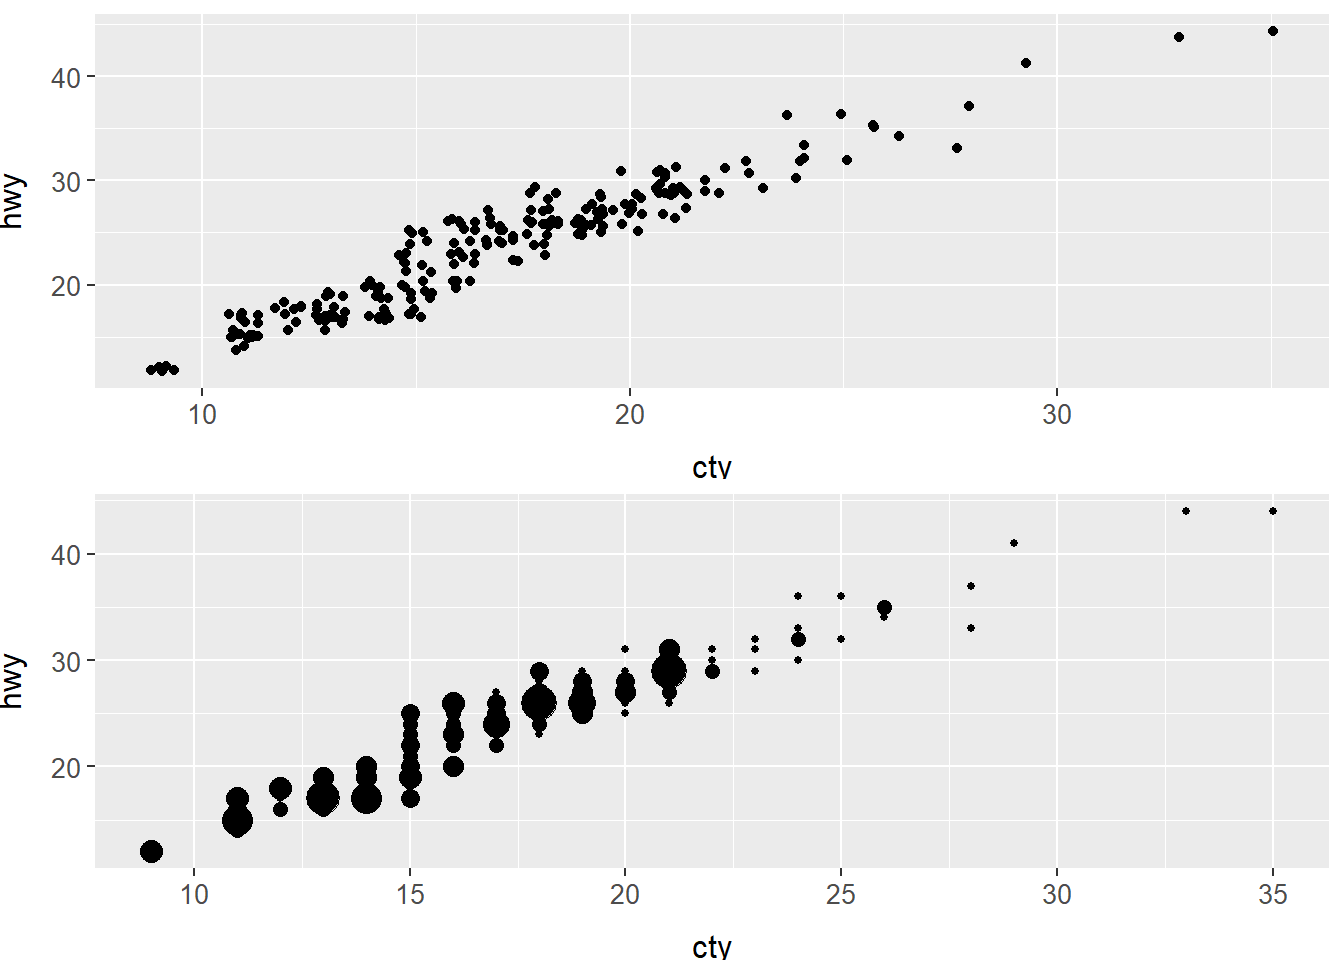
\includegraphics{r4ds_files/figure-latex/unnamed-chunk-36-1.pdf}

Para contornar o problema da sobreposição de pontos, \texttt{geom\_jitter} adiciona um pequeno ruído aleatório aos dados, enquanto o \texttt{geom\_count} contabiliza os pontos sobrepostos e altera o tamanho dos pontos conforme a quantidade.

\end{solution}

\hypertarget{exr1-8-4}{%
\subsection*{Exercício 1.8.4}\label{exr1-8-4}}
\addcontentsline{toc}{subsection}{Exercício 1.8.4}

Qual é o ajuste de posição padrão para \texttt{geom\_boxplot()}? Crie uma visualização do conjunto de dados \texttt{mpg} que demonstre isso.

\begin{solution}
Conforme pode ser visto em \texttt{?geom\_boxplot}, a \texttt{position} padrão é a \texttt{dodge2}.

\begin{Shaded}
\begin{Highlighting}[]
\FunctionTok{ggplot}\NormalTok{(}\AttributeTok{data =}\NormalTok{ mpg, }\AttributeTok{mapping =} \FunctionTok{aes}\NormalTok{(}\AttributeTok{x =}\NormalTok{ class, }\AttributeTok{y =}\NormalTok{ hwy)) }\SpecialCharTok{+}
    \FunctionTok{geom\_boxplot}\NormalTok{() }\SpecialCharTok{+}
\NormalTok{    tema}
\end{Highlighting}
\end{Shaded}

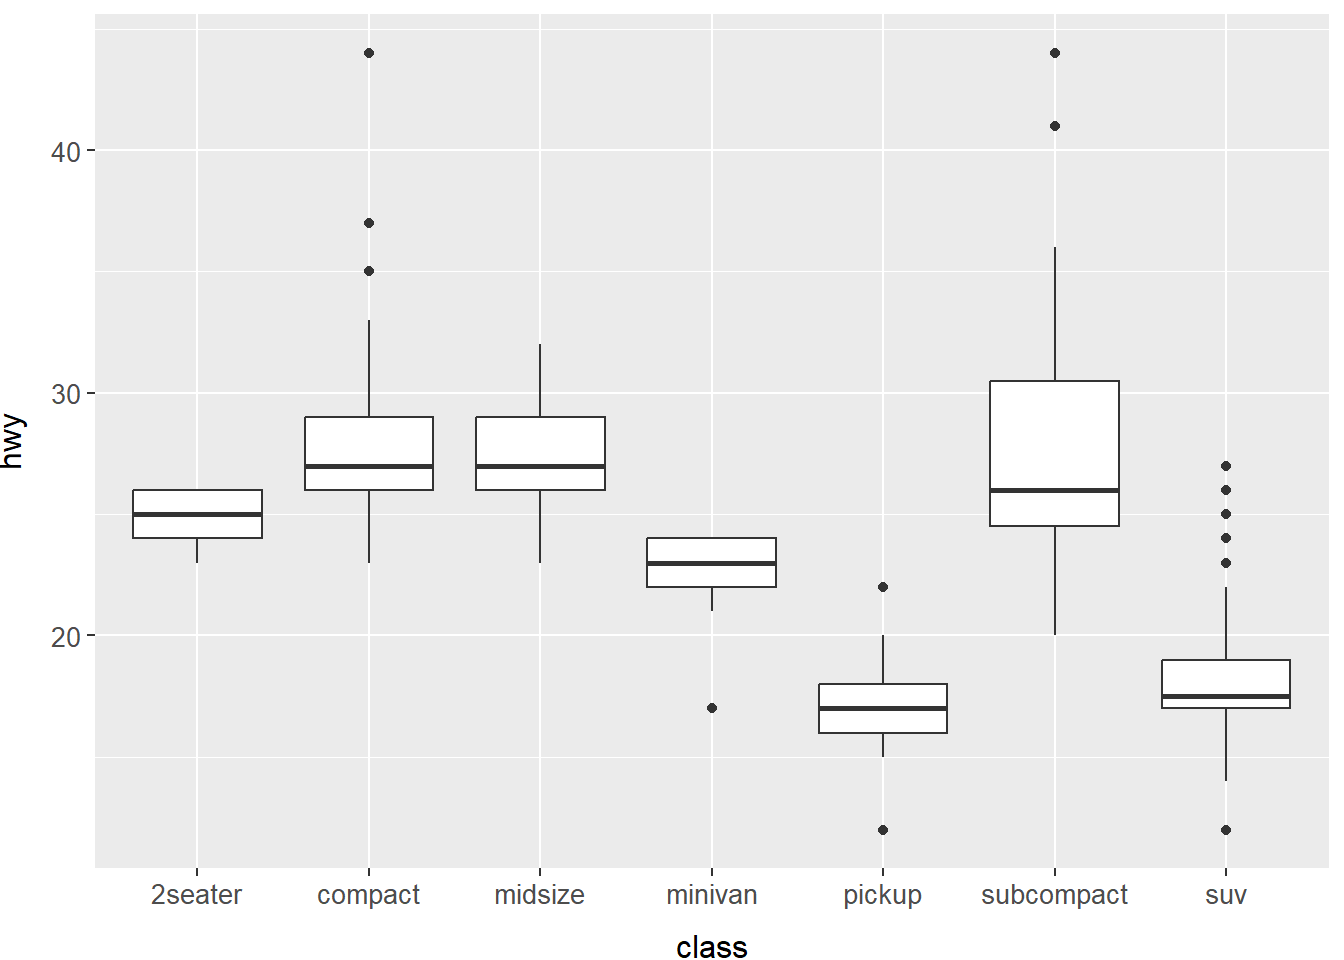
\includegraphics{r4ds_files/figure-latex/unnamed-chunk-37-1.pdf}
\end{solution}

\hypertarget{sistemas-de-coordenadas}{%
\section{Sistemas de coordenadas}\label{sistemas-de-coordenadas}}

\hypertarget{exr1-9-1}{%
\subsection*{Exercício 1.9.1}\label{exr1-9-1}}
\addcontentsline{toc}{subsection}{Exercício 1.9.1}

Transforme um gráfico de barras empilhadas em um gráfico de pizza usando \texttt{coord\_polar()}.

\begin{solution}
\leavevmode

\begin{Shaded}
\begin{Highlighting}[]
\FunctionTok{ggplot}\NormalTok{(}\AttributeTok{data =}\NormalTok{ diamonds, }\AttributeTok{mapping =} \FunctionTok{aes}\NormalTok{(}\AttributeTok{x =}\NormalTok{ cut, }\AttributeTok{fill =}\NormalTok{ cut)) }\SpecialCharTok{+}
    \FunctionTok{geom\_bar}\NormalTok{(}\AttributeTok{show.legend =} \ConstantTok{FALSE}\NormalTok{, }\AttributeTok{width =} \DecValTok{1}\NormalTok{) }\SpecialCharTok{+}
    \FunctionTok{coord\_polar}\NormalTok{() }\SpecialCharTok{+}
    \FunctionTok{labs}\NormalTok{(}\AttributeTok{x =} \ConstantTok{NULL}\NormalTok{, }\AttributeTok{y =} \ConstantTok{NULL}\NormalTok{) }\SpecialCharTok{+}
    \FunctionTok{theme}\NormalTok{(}\AttributeTok{aspect.ratio =} \DecValTok{1}\NormalTok{) }\SpecialCharTok{+}
\NormalTok{    tema}
\end{Highlighting}
\end{Shaded}

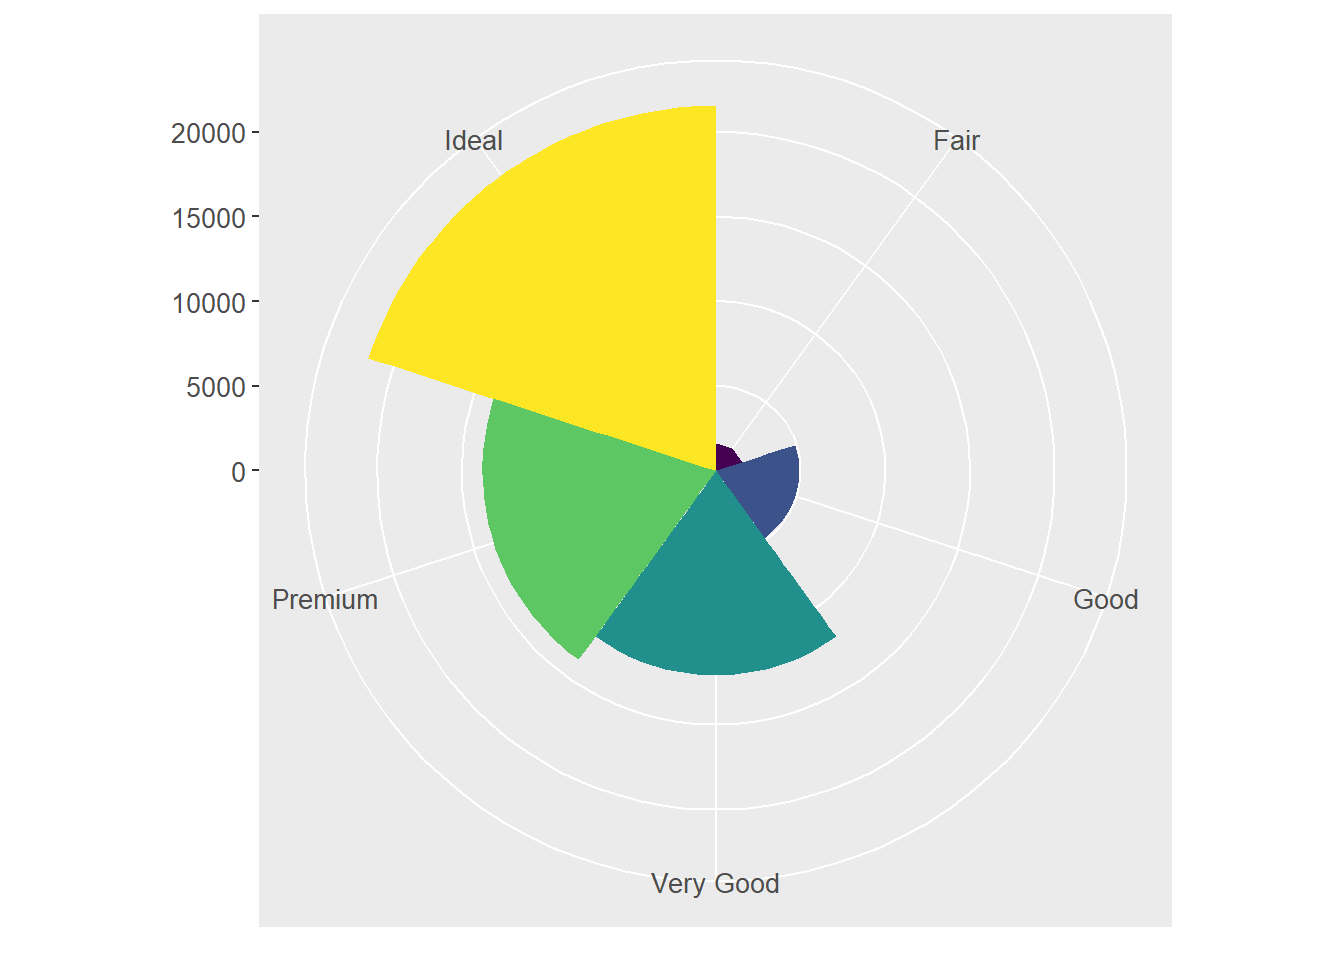
\includegraphics{r4ds_files/figure-latex/unnamed-chunk-38-1.pdf}

\end{solution}

\hypertarget{exr1-9-2}{%
\subsection*{Exercício 1.9.2}\label{exr1-9-2}}
\addcontentsline{toc}{subsection}{Exercício 1.9.2}

O que \texttt{labs()} faz? Leia a documentação.

\begin{solution}
Usando o comando \texttt{?labs}, vimos que esta função é utilizada para definir labels do gráfico, como título, subtítulo, títulos de eixos, etc.
\end{solution}

\hypertarget{exr1-9-3}{%
\subsection*{Exercício 1.9.3}\label{exr1-9-3}}
\addcontentsline{toc}{subsection}{Exercício 1.9.3}

Qual é a diferença entre \texttt{coord\_quickmap()} e \texttt{coord\_map()}?

\begin{solution}
Usando o comando \texttt{?coord\_map}, notamos que a diferença é que enquanto \texttt{coord\_map()} não preserva linhas retas, sendo assim, mais custoso computacionalmente, o \texttt{coord\_quickmap()} o faz.
\end{solution}

\hypertarget{exr1-9-4}{%
\subsection*{Exercício 1.9.4}\label{exr1-9-4}}
\addcontentsline{toc}{subsection}{Exercício 1.9.4}

O que o gráfico a seguir lhe diz sobre a relação entre \texttt{mpg} de cidade e estrada? Por que \texttt{coord\_fixed()} é importante? O que \texttt{geom\_abline()} faz?

\begin{Shaded}
\begin{Highlighting}[]
\FunctionTok{ggplot}\NormalTok{(}\AttributeTok{data =}\NormalTok{ mpg, }\AttributeTok{mapping =} \FunctionTok{aes}\NormalTok{(}\AttributeTok{x =}\NormalTok{ cty, }\AttributeTok{y =}\NormalTok{ hwy)) }\SpecialCharTok{+}
    \FunctionTok{geom\_point}\NormalTok{() }\SpecialCharTok{+}
    \FunctionTok{geom\_abline}\NormalTok{() }\SpecialCharTok{+}
    \FunctionTok{coord\_fixed}\NormalTok{(}\AttributeTok{ratio =} \DecValTok{1}\NormalTok{, }\AttributeTok{xlim =} \FunctionTok{c}\NormalTok{(}\DecValTok{5}\NormalTok{, }\DecValTok{45}\NormalTok{), }\AttributeTok{ylim =} \FunctionTok{c}\NormalTok{(}\DecValTok{5}\NormalTok{, }\DecValTok{45}\NormalTok{)) }\SpecialCharTok{+}
\NormalTok{    tema}
\end{Highlighting}
\end{Shaded}

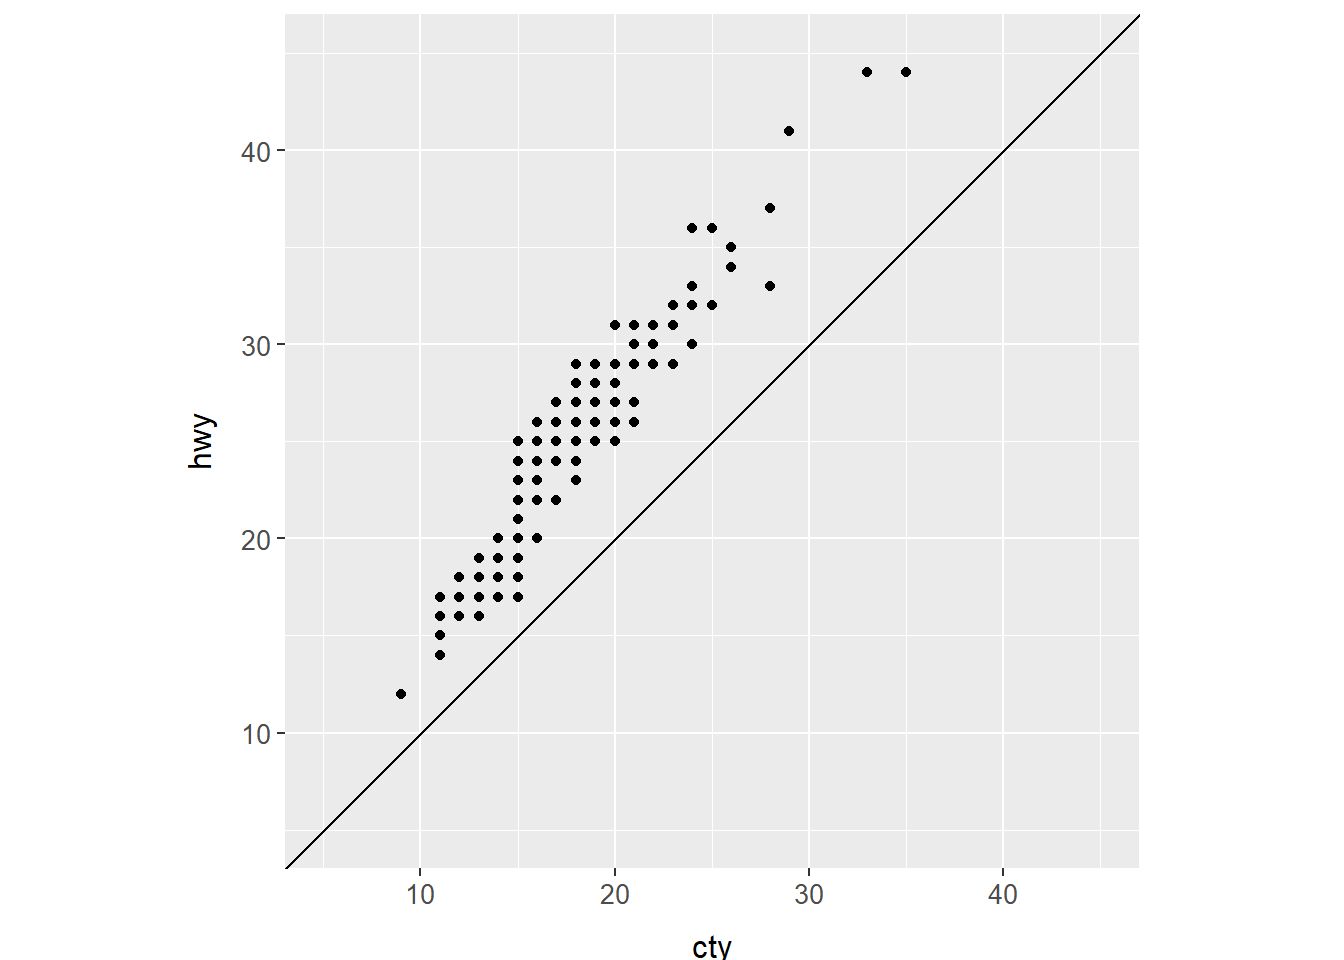
\includegraphics{r4ds_files/figure-latex/unnamed-chunk-39-1.pdf}

\begin{solution}
O gráfico mostra a relação entre a eficiência na cidade e na estrada. O \texttt{coord\_fixed()} força que seja mantida uma proporção entre os eixos x e y, isto é, garante que uma unidade no eixo y corresponda a um número determinado de unidades no eixo x. A razão padrão é 1. Já o \texttt{geom\_abline()} define uma linha de referência diagonal ao gráfico, no nosso caso, a linha é a reta dada por \(y - x = 0\).
\end{solution}

\hypertarget{a-gramuxe1tica-em-camadas-de-gruxe1ficos}{%
\section{A gramática em camadas de gráficos}\label{a-gramuxe1tica-em-camadas-de-gruxe1ficos}}

Não temos exercícios nesta seção.

\hypertarget{fluxo-de-trabalho-o-buxe1sico}{%
\chapter{Fluxo de trabalho: o básico}\label{fluxo-de-trabalho-o-buxe1sico}}

\hypertarget{o-buxe1sico-de-programauxe7uxe3o}{%
\section{O básico de programação}\label{o-buxe1sico-de-programauxe7uxe3o}}

Não temos exercícios nesta seção.

\hypertarget{o-que-huxe1-em-um-nome}{%
\section{O que há em um nome?}\label{o-que-huxe1-em-um-nome}}

Não temos exercícios nesta seção.

\hypertarget{chamando-funuxe7uxf5es}{%
\section{Chamando funções}\label{chamando-funuxe7uxf5es}}

\hypertarget{exr2-3-1}{%
\subsection*{Exercício 2.3.1}\label{exr2-3-1}}
\addcontentsline{toc}{subsection}{Exercício 2.3.1}

Por que esse código não funciona?

\begin{verbatim}
my_variable <- 10
my_varIable
\end{verbatim}

\begin{solution}
Foi atribuído um valor à variável \texttt{my\_variable}, contudo depois tentou-se utilizar essa variável, porém a escrita está incorreta e o \texttt{R} não reconheceu a variável.
O \texttt{R} diferencia letras maiúsculas e minúsculas, isto é, as variáveis \texttt{my\_variable} e \texttt{my\_varIable} são distintas.
\end{solution}

\hypertarget{exr2-3-2}{%
\subsection*{Exercício 2.3.2}\label{exr2-3-2}}
\addcontentsline{toc}{subsection}{Exercício 2.3.2}

Ajuste cada um dos seguintes comandos de \texttt{R} para que executem corretamente.

\begin{verbatim}
library(tidyverse)

ggplot(dota = mpg) +
    geom_point(mapping = aes(x = displ, y = hwy))
    
filter(mpg, cyl = 8)
filter(diamond, carat > 3)
\end{verbatim}

\begin{solution}
\leavevmode

\begin{Shaded}
\begin{Highlighting}[]
\FunctionTok{library}\NormalTok{(tidyverse)}

\FunctionTok{ggplot}\NormalTok{(}\AttributeTok{data =}\NormalTok{ mpg) }\SpecialCharTok{+}
    \FunctionTok{geom\_point}\NormalTok{(}\AttributeTok{mapping =} \FunctionTok{aes}\NormalTok{(}\AttributeTok{x =}\NormalTok{ displ, }\AttributeTok{y =}\NormalTok{ hwy))}
\end{Highlighting}
\end{Shaded}

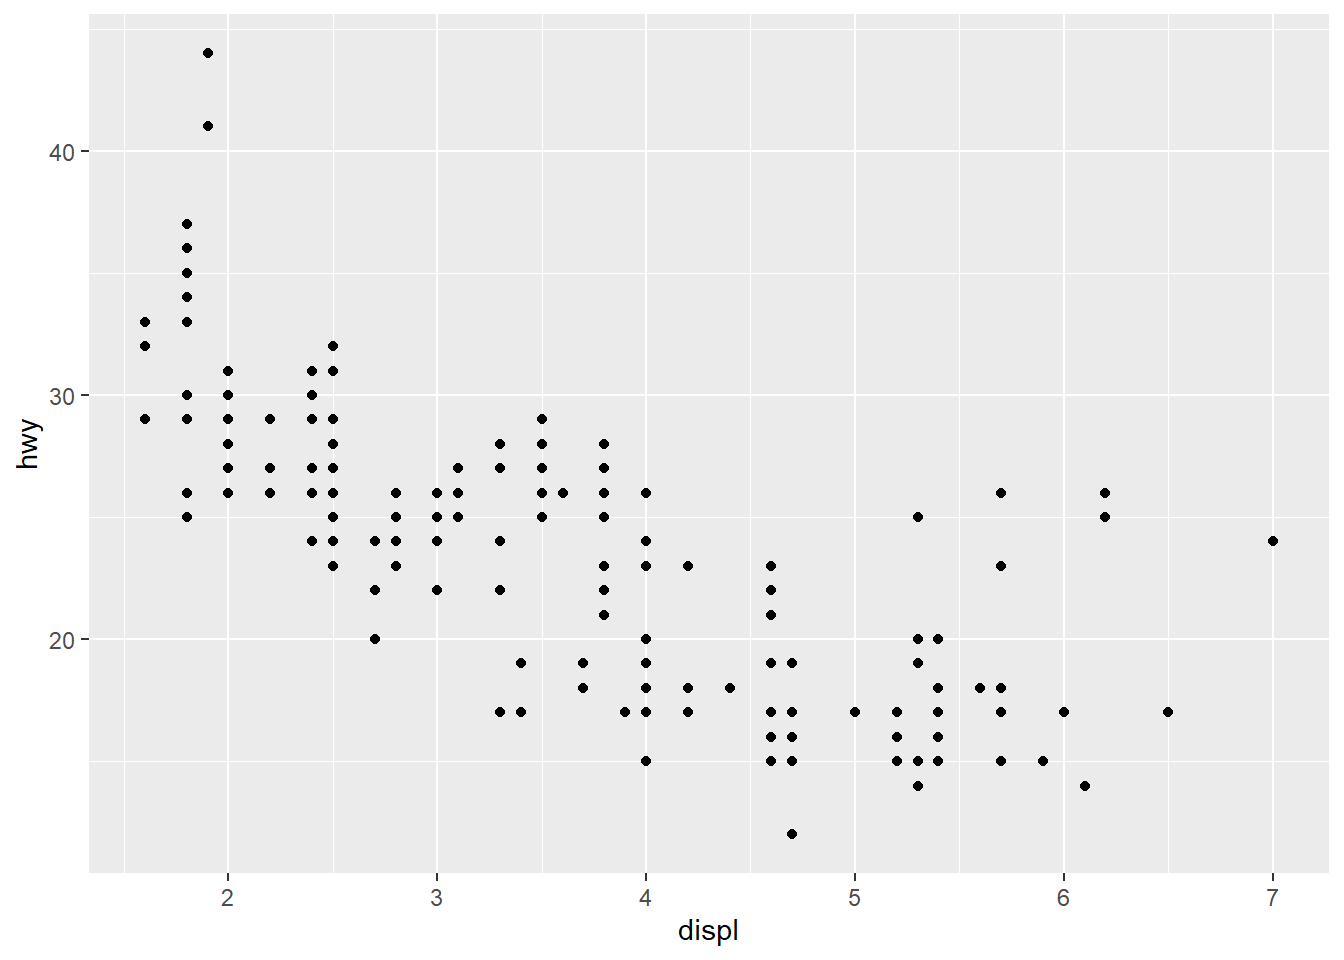
\includegraphics{r4ds_files/figure-latex/unnamed-chunk-40-1.pdf}

\begin{Shaded}
\begin{Highlighting}[]
\FunctionTok{filter}\NormalTok{(mpg, cyl }\SpecialCharTok{==} \DecValTok{8}\NormalTok{)}
\end{Highlighting}
\end{Shaded}

\begin{verbatim}
## # A tibble: 70 x 11
##    manufacturer model      displ  year   cyl trans drv     cty   hwy fl    class
##    <chr>        <chr>      <dbl> <int> <int> <chr> <chr> <int> <int> <chr> <chr>
##  1 audi         a6 quattro   4.2  2008     8 auto~ 4        16    23 p     mids~
##  2 chevrolet    c1500 sub~   5.3  2008     8 auto~ r        14    20 r     suv  
##  3 chevrolet    c1500 sub~   5.3  2008     8 auto~ r        11    15 e     suv  
##  4 chevrolet    c1500 sub~   5.3  2008     8 auto~ r        14    20 r     suv  
##  5 chevrolet    c1500 sub~   5.7  1999     8 auto~ r        13    17 r     suv  
##  6 chevrolet    c1500 sub~   6    2008     8 auto~ r        12    17 r     suv  
##  7 chevrolet    corvette     5.7  1999     8 manu~ r        16    26 p     2sea~
##  8 chevrolet    corvette     5.7  1999     8 auto~ r        15    23 p     2sea~
##  9 chevrolet    corvette     6.2  2008     8 manu~ r        16    26 p     2sea~
## 10 chevrolet    corvette     6.2  2008     8 auto~ r        15    25 p     2sea~
## # i 60 more rows
\end{verbatim}

\begin{Shaded}
\begin{Highlighting}[]
\FunctionTok{filter}\NormalTok{(diamonds, carat }\SpecialCharTok{\textgreater{}} \DecValTok{3}\NormalTok{)}
\end{Highlighting}
\end{Shaded}

\begin{verbatim}
## # A tibble: 32 x 10
##    carat cut     color clarity depth table price     x     y     z
##    <dbl> <ord>   <ord> <ord>   <dbl> <dbl> <int> <dbl> <dbl> <dbl>
##  1  3.01 Premium I     I1       62.7    58  8040  9.1   8.97  5.67
##  2  3.11 Fair    J     I1       65.9    57  9823  9.15  9.02  5.98
##  3  3.01 Premium F     I1       62.2    56  9925  9.24  9.13  5.73
##  4  3.05 Premium E     I1       60.9    58 10453  9.26  9.25  5.66
##  5  3.02 Fair    I     I1       65.2    56 10577  9.11  9.02  5.91
##  6  3.01 Fair    H     I1       56.1    62 10761  9.54  9.38  5.31
##  7  3.65 Fair    H     I1       67.1    53 11668  9.53  9.48  6.38
##  8  3.24 Premium H     I1       62.1    58 12300  9.44  9.4   5.85
##  9  3.22 Ideal   I     I1       62.6    55 12545  9.49  9.42  5.92
## 10  3.5  Ideal   H     I1       62.8    57 12587  9.65  9.59  6.03
## # i 22 more rows
\end{verbatim}

\end{solution}

\hypertarget{exr2-3-3}{%
\subsection*{Exercício 2.3.3}\label{exr2-3-3}}
\addcontentsline{toc}{subsection}{Exercício 2.3.3}

Pressione Alt-Shift-K. O que acontece? Como você pode chegar ao mesmo resultado usando os menus?

\begin{solution}
x
\end{solution}

\hypertarget{transformauxe7uxe3o-de-dados-com-dplyr}{%
\chapter{\texorpdfstring{Transformação de dados com \texttt{dplyr}}{Transformação de dados com dplyr}}\label{transformauxe7uxe3o-de-dados-com-dplyr}}

\hypertarget{fluxo-de-trabalho-scripts}{%
\chapter{Fluxo de trabalho: scripts}\label{fluxo-de-trabalho-scripts}}

\hypertarget{anuxe1lise-exploratuxf3ria-de-dados}{%
\chapter{Análise exploratória de dados}\label{anuxe1lise-exploratuxf3ria-de-dados}}

\hypertarget{fluxo-de-trabalho-projetos}{%
\chapter{Fluxo de trabalho: projetos}\label{fluxo-de-trabalho-projetos}}

\hypertarget{part-wrangle}{%
\part{Wrangle}\label{part-wrangle}}

\hypertarget{tibbles-com-tibble}{%
\chapter{\texorpdfstring{Tibbles com \texttt{tibble}}{Tibbles com tibble}}\label{tibbles-com-tibble}}

\hypertarget{importando-dados-com-readr}{%
\chapter{\texorpdfstring{Importando dados com \texttt{readr}}{Importando dados com readr}}\label{importando-dados-com-readr}}

\hypertarget{arrumando-dados-com-tidyr}{%
\chapter{\texorpdfstring{Arrumando dados com \texttt{tidyr}}{Arrumando dados com tidyr}}\label{arrumando-dados-com-tidyr}}

\hypertarget{dados-relacionais-com-dplyr}{%
\chapter{\texorpdfstring{Dados relacionais com \texttt{dplyr}}{Dados relacionais com dplyr}}\label{dados-relacionais-com-dplyr}}

\hypertarget{strings-com-stringr}{%
\chapter{\texorpdfstring{Strings com \texttt{stringr}}{Strings com stringr}}\label{strings-com-stringr}}

\hypertarget{fatores-com-forcats}{%
\chapter{\texorpdfstring{Fatores com \texttt{forcats}}{Fatores com forcats}}\label{fatores-com-forcats}}

\hypertarget{datas-e-horas-com-lubridate}{%
\chapter{\texorpdfstring{Datas e horas com \texttt{lubridate}}{Datas e horas com lubridate}}\label{datas-e-horas-com-lubridate}}

\hypertarget{part-programar}{%
\part{Programar}\label{part-programar}}

\hypertarget{pipes-com-magrittr}{%
\chapter{\texorpdfstring{Pipes com \texttt{magrittr}}{Pipes com magrittr}}\label{pipes-com-magrittr}}

\hypertarget{funuxe7uxf5es}{%
\chapter{Funções}\label{funuxe7uxf5es}}

\hypertarget{vetores}{%
\chapter{Vetores}\label{vetores}}

\hypertarget{iterauxe7uxe3o-com-purrr}{%
\chapter{\texorpdfstring{Iteração com \texttt{purrr}}{Iteração com purrr}}\label{iterauxe7uxe3o-com-purrr}}

\hypertarget{part-modelar}{%
\chapter{(PART) Modelar}\label{part-modelar}}

\hypertarget{o-buxe1sico-de-modelos-com-modelr}{%
\chapter{\texorpdfstring{O básico de modelos com \texttt{modelr}}{O básico de modelos com modelr}}\label{o-buxe1sico-de-modelos-com-modelr}}

\hypertarget{construuxe7uxe3o-de-modelos}{%
\chapter{Construção de modelos}\label{construuxe7uxe3o-de-modelos}}

\hypertarget{muitos-modelos-com-purrr-e-broom}{%
\chapter{\texorpdfstring{Muitos modelos com \texttt{purrr} e \texttt{broom}}{Muitos modelos com purrr e broom}}\label{muitos-modelos-com-purrr-e-broom}}

\hypertarget{part-comunicar}{%
\part{Comunicar}\label{part-comunicar}}

\hypertarget{r-markdown}{%
\chapter{R Markdown}\label{r-markdown}}

\hypertarget{gruxe1ficos-para-comunicauxe7uxe3o-com-ggplot2}{%
\chapter{\texorpdfstring{Gráficos para comunicação com \texttt{ggplot2}}{Gráficos para comunicação com ggplot2}}\label{gruxe1ficos-para-comunicauxe7uxe3o-com-ggplot2}}

\hypertarget{formatos-r-markdown}{%
\chapter{Formatos R Markdown}\label{formatos-r-markdown}}

\hypertarget{fluxo-de-trabalho-de-r-markdown}{%
\chapter{Fluxo de trabalho de R Markdown}\label{fluxo-de-trabalho-de-r-markdown}}

  \bibliography{latex/book.bib,latex/packages.bib}

\printindex

\end{document}
